 %% abtex2-modelo-trabalho-academico.tex, v-1.9.2 laurocesar

%% Copyright 2012-2014 by abnTeX2 group at http://abntex2.googlecode.com/ 
%%
%% This work may be distributed and/or modified under the
%% conditions of the LaTeX Project Public License, either version 1.3
%% of this license or (at your option) any later version.
%% The latest version of this license is in
%%   http://www.latex-project.org/lppl.txt
%% and version 1.3 or later is part of all distributions of LaTeX
%% version 2005/12/01 or later.
%%
%% This work has the LPPL maintenance status `maintained'.
%% 
%% The Current Maintainer of this work is the abnTeX2 team, led
%% by Lauro César Araujo. Further information are available on 
%% http://abntex2.googlecode.com/
%%
%% This work consists of the files abntex2-modelo-trabalho-academico.tex,
%% abntex2-modelo-include-comandos and abntex2-modelo-references.bib
%%

% ------------------------------------------------------------------------
% ------------------------------------------------------------------------
% abnTeX2: Modelo de Trabalho Academico (tese de doutorado, dissertacao de
% mestrado e trabalhos monograficos em geral) em conformidade com 
% ABNT NBR 14724:2011: Informacao e documentacao - Trabalhos academicos -
% Apresentacao
% ------------------------------------------------------------------------
% ------------------------------------------------------------------------

\documentclass[
	% -- opções da classe memoir --
	12pt,				% tamanho da fonte
	openright,			% capítulos começam em pág ímpar (insere página vazia caso preciso)
	twoside,			% para impressão em verso e anverso. Oposto a oneside
	a4paper,			% tamanho do papel. 
	% -- opções da classe abntex2 --
	%chapter=TITLE,		% títulos de capítulos convertidos em letras maiúsculas
	%section=TITLE,		% títulos de seções convertidos em letras maiúsculas
	%subsection=TITLE,	% títulos de subseções convertidos em letras maiúsculas
	%subsubsection=TITLE,% títulos de subsubseções convertidos em letras maiúsculas
	% -- opções do pacote babel --
	english,			% idioma adicional para hifenização
	french,				% idioma adicional para hifenização
	spanish,			% idioma adicional para hifenização
	brazil				% o último idioma é o principal do documento
	]{abntex2}
%https://code.google.com/p/abntex2/wiki/Texmaker
% ---
% Pacotes básicos 
% ---
\usepackage{lmodern}			% Usa a fonte Latin Modern			
\usepackage[T1]{fontenc}		% Selecao de codigos de fonte.
\usepackage[utf8]{inputenc}		% Codificacao do documento (conversão automática dos acentos)
\usepackage{lastpage}			% Usado pela Ficha catalográfica
\usepackage{indentfirst}		% Indenta o primeiro parágrafo de cada seção.
\usepackage{color}				% Controle das cores
\usepackage{graphicx}			% Inclusão de gráficos
\usepackage{microtype} 			% para melhorias de justificação
\usepackage{url}
\usepackage[table,xcdraw]{xcolor}
\usepackage{enumitem}

% ---
		
% ---
% Pacotes adicionais, usados apenas no âmbito do Modelo Canônico do abnteX2
% ---
\usepackage{lipsum}				% para geração de dummy text
% ---

% ---
% Pacotes de citações
% ---
\usepackage[brazilian,hyperpageref]{backref}	 % Paginas com as citações na bibl
\usepackage[alf]{abntex2cite}	% Citações padrão ABNT
\usepackage{float}

%%%%%%%%%%% syntax highlight %%%%%%%%%%%%%%%%%%%%%%%%%%%%%%%%%%%%%%%%%%%%%%%%%%%%%


\usepackage[procnames]{listings}

\definecolor{keywords}{RGB}{255,0,90}
\definecolor{comments}{RGB}{0,0,113}
\definecolor{red}{RGB}{160,0,0}
\definecolor{green}{RGB}{0,150,0}

\lstset{language=Python, 
basicstyle=\ttfamily\tiny, 
keywordstyle=\color{keywords},
commentstyle=\color{comments},
stringstyle=\color{red},
showstringspaces=false,
frame=single, 
identifierstyle=\color{green},
procnamekeys={def,class}}


%%%%%%%%%%%%%%%%%%%%%%%%%%%%%%%%%%%%%%%%%%%%%%%%%%%%%%% 


% --- 
% CONFIGURAÇÕES DE PACOTES
% --- 

% ---
% Configurações do pacote backref
% Usado sem a opção hyperpageref de backref
\renewcommand{\backrefpagesname}{Citado na(s) página(s):~}
% Texto padrão antes do número das páginas
\renewcommand{\backref}{}
% Define os textos da citação
\renewcommand*{\backrefalt}[4]{
	\ifcase #1 %
		Nenhuma citação no texto.%
	\or
		Citado na página #2.%
	\else
		Citado #1 vezes nas páginas #2.%
	\fi}%
% ---

% ---
% Informações de dados para CAPA e FOLHA DE ROSTO
% ---
\titulo{Luteria Composicional de algoritmos pós-tonais }
\autor{Guilherme Rafael Soares}
%\local{Brasil}
\data{29 de abril 2015.}
\orientador{Prof. Dr. Daniel Quaranta}
%\coorientador{Equipe \abnTeX}
\instituicao{%
  UFJF - Universidade Federal de Juiz de Fora
  \par
  Instituto de Artes e Design
  \par
  Programa de Pós-Graduação em Artes, Cultura e Linguagens}
\tipotrabalho{Dissertação (Mestrado)}
% O preambulo deve conter o tipo do trabalho, o objetivo, 
% o nome da instituição e a área de concentração 
\preambulo{Dissertação apresentada ao \textbf{Programa de Pós-Graduação em Artes, Cultura e Linguagens}, Área de Concentração: \textbf{Teorias e Processos Poéticos Interdisciplinares}, Linha de pesquisa: \textbf{ARTES VISUAIS, MÚSICA E TECNOLOGIA}, da Universidade Federal de Juiz de Fora para obtenção do grau de \textbf{Mestre}. }
% ---


% ---
% Configurações de aparência do PDF final

% alterando o aspecto da cor azul
\definecolor{blue}{RGB}{41,5,195}

% informações do PDF
\makeatletter
\hypersetup{
     	%pagebackref=true,
		pdftitle={\@title}, 
		pdfauthor={\@author},
    	pdfsubject={\imprimirpreambulo},
	    pdfcreator={LaTeX with abnTeX2},
		pdfkeywords={abnt}{latex}{abntex}{abntex2}{trabalho acadêmico}, 
		colorlinks=true,       		% false: boxed links; true: colored links
    	linkcolor=blue,          	% color of internal links
    	citecolor=blue,        		% color of links to bibliography
    	filecolor=magenta,      		% color of file links
		urlcolor=blue,
		bookmarksdepth=4
}
\makeatother
% --- 

% --- 
% Espaçamentos entre linhas e parágrafos 
% --- 

% O tamanho do parágrafo é dado por:
\setlength{\parindent}{1.3cm}

% Controle do espaçamento entre um parágrafo e outro:
\setlength{\parskip}{0.2cm}  % tente também \onelineskip

% ---
% compila o indice
% ---
\makeindex
% ---

% ----
% Início do documento
% ----
\begin{document}

% Retira espaço extra obsoleto entre as frases.
\frenchspacing 

% ----------------------------------------------------------
% ELEMENTOS PRÉ-TEXTUAIS
% ----------------------------------------------------------
% \pretextual

% ---
% Capa
% ---
\imprimircapa
% ---


% ---
% Folha de rosto
% (o * indica que haverá a ficha bibliográfica)
% ---
\imprimirfolhaderosto*
% ---

% ---
% Inserir a ficha bibliografica
% ---

% Isto é um exemplo de Ficha Catalográfica, ou ``Dados internacionais de
% catalogação-na-publicação''. Você pode utilizar este modelo como referência. 
% Porém, provavelmente a biblioteca da sua universidade lhe fornecerá um PDF
% com a ficha catalográfica definitiva após a defesa do trabalho. Quando estiver
% com o documento, salve-o como PDF no diretório do seu projeto e substitua todo
% o conteúdo de implementação deste arquivo pelo comando abaixo:
%
% \begin{fichacatalografica}
%     \includepdf{fig_ficha_catalografica.pdf}
% \end{fichacatalografica}
\begin{fichacatalografica}
	\vspace*{\fill}					% Posição vertical
	\hrule							% Linha horizontal
	\begin{center}					% Minipage Centralizado
	\begin{minipage}[c]{12.5cm}		% Largura
	
	\imprimirautor
	
	\hspace{0.5cm} \imprimirtitulo  / \imprimirautor. --
	\imprimirlocal, \imprimirdata-
	
	\hspace{0.5cm} \pageref{LastPage} p. : il. (algumas color.) ; 30 cm.\\
	
	\hspace{0.5cm} \imprimirorientadorRotulo~\imprimirorientador\\
	
	\hspace{0.5cm}
	\parbox[t]{\textwidth}{\imprimirtipotrabalho~--~\imprimirinstituicao,
	\imprimirdata.}\\
	
	\hspace{0.5cm}
		1. Palavra-chave1.
		2. Palavra-chave2.
		I. Orientador: Prof. Dr. Daniel Quaranta
		II. UFJF - Universidade Federal de Juiz de Fora.
		III. Instituto de Artes e Design
		IV. \imprimirtitulo \\ 			
	
	\hspace{8.75cm} CDU 02:141:005.7\\
	
	\end{minipage}
	\end{center}
	\hrule
\end{fichacatalografica}
% ---

% ---
% Inserir errata
% ---
%\begin{errata}
%Elemento opcional da \citeonline[4.2.1.2]{NBR14724:2011}. Exemplo:
%
%\vspace{\onelineskip}
%
%FERRIGNO, C. R. A. \textbf{Tratamento de neoplasias ósseas apendiculares com
%reimplantação de enxerto ósseo autólogo autoclavado associado ao plasma
%rico em plaquetas}: estudo crítico na cirurgia de preservação de membro em
%cães. 2011. 128 f. Tese (Livre-Docência) - Faculdade de Medicina Veterinária e
%Zootecnia, Universidade de São Paulo, São Paulo, 2011.
%
%\begin{table}[htb]
%\center
%\footnotesize
%\begin{tabular}{|p{1.4cm}|p{1cm}|p{3cm}|p{3cm}|}
%  \hline
%   \textbf{Folha} & \textbf{Linha}  & \textbf{Onde se lê}  & \textbf{Leia-se}  \\
%    \hline
%    1 & 10 & auto-conclavo & autoconclavo\\
%   \hline
%\end{tabular}
%\end{table}

%\end{errata}
% ---

% ---
% Inserir folha de aprovação
% ---

% Isto é um exemplo de Folha de aprovação, elemento obrigatório da NBR
% 14724/2011 (seção 4.2.1.3). Você pode utilizar este modelo até a aprovação
% do trabalho. Após isso, substitua todo o conteúdo deste arquivo por uma
% imagem da página assinada pela banca com o comando abaixo:
%
% \includepdf{folhadeaprovacao_final.pdf}
%
%\begin{folhadeaprovacao}
%
%  \begin{center}
%    {\ABNTEXchapterfont\large\imprimirautor}

%    \vspace*{\fill}\vspace*{\fill}
%    \begin{center}
%      \ABNTEXchapterfont\bfseries\Large\imprimirtitulo
%    \end{center}
%    \vspace*{\fill}
    
%    \hspace{.45\textwidth}
%    \begin{minipage}{.5\textwidth}
%        \imprimirpreambulo
%    \end{minipage}%
%    \vspace*{\fill}
%   \end{center}
        
%   Trabalho aprovado \imprimirlocal, 13 de fevereiro de 2015:

%   \assinatura{\textbf{\imprimirorientador} \\ Orientador} 
%   \assinatura{\textbf{Prof. Dr. Alexandre Sperandéo Fenerich} \\ Titular interno}
%   \assinatura{\textbf{Prof. Dr. Cristiano Severo Figueiró} \\ Titular externo}
   %\assinatura{\textbf{Professor} \\ Convidado 3}
   %\assinatura{\textbf{Professor} \\ Convidado 4}
      
%   \begin{center}
%    \vspace*{0.5cm}
%    {\large\imprimirlocal}
%    \par
%    {\large\imprimirdata}
%    \vspace*{1cm}
%  \end{center}
  
%\end{folhadeaprovacao}
% ---

% ---
% Dedicatória
% ---
%\begin{dedicatoria}
%   \vspace*{\fill}
 %  \centering
 %  \noindent
 %  \textit{ Este trabalho é dedicado às crianças adultas que,\\
 %  quando pequenas, sonharam em se tornar cientistas.} \vspace*{\fill}
%\end{dedicatoria}
% ---

% ---
% Agradecimentos
% ---
\begin{agradecimentos}
Seu nome consta aqui num papelzinho que guardei no bolso, junto com a senha da internet da biblioteca.
Quando você vier buscar o seu papel traga também suas anotações com as quais escreveremos a continuação daquilo tudo que talvez tenha ficado inacabado.
Jogando os papéis para o alto faremos a música que aqui não coube.
Alguém (cujo nome também está escrito) irá tomar nota disso tudo, e contar uma versão entusiasmada dessa história, com os detalhes que faltavam, sem esperar de mim nada em troca.
\end{agradecimentos}
% ---

% ---
% Epígrafe cortazar
% ---
%\begin{epigrafe}
 %   \vspace*{\fill}
%	\begin{flushright}
%		\textit{Epígrafe? Um desenho de um LP preferido - contracapa: ou 78 restrições seriam outras: antes de 0,618: se é possível esquecer: e há gosto em esquecer: algo isola. eu isolei?: um algarismo por dentro. (Lucida Sans) }
%	\end{flushright}
%\end{epigrafe}



% ---

% ---
% RESUMOS
% ---

% resumo em português

\setlength{\absparsep}{18pt} % ajusta o espaçamento dos parágrafos do resumo



\begin{resumo}


Esta pesquisa sistematiza um catálogo de experimentos constituído de estudos musicais e seus algoritmos geradores, organizando procedimentos para composição assistida por computador orientados por regras derivadas de análises musicais de contexto pós-tonal.


Os procedimentos são inspirados em apontamentos de estudos sobre pós-tonalidade no compositor Béla Bartók, encontrados nas obras de \citeonline{lendvai1971bela,antokoletz1984music,cohn1991bartok} e  \citeonline{suchoff2004bartok}. Problematizam-se aqui os conceitos de ciclos intervalares, eixos de simetria, polimodalismo e peculiaridades de coleções referenciais de classes de altura - conforme sugestões de 
\citeonline{forte1973structure, straus2004} e \citeonline{susanni_antokoletz2012music}.

São detalhadas questões computacionais para esta implementação, utilizando como base as ferramentas OpenMusic e biblioteca Python Music21. 

Um legado em código aberto fica disponível para continuidades possíveis deste trabalho.


 \textbf{Palavras-chaves}: Música algorítmica. Pós-tonalismo. Teoria dos conjuntos. Pitch class theory. Luteria. Composição assistida por computador. Musicologia assistida por computador. Open Music. Music21. Software livre. Béla Bartók.
\end{resumo}

%%%%%%%%%% traduçoes resumo

% resumo em inglês
\begin{resumo}[Abstract]
 \begin{otherlanguage*}{english}


This research produces a catalog of experiments in musical studies and its related generative algorithms, organizing procedures for computer aided composition oriented by constraints extracted from post-tonal musical analyses.

The procedures are inspired by post-tonality studies of Béla Bartók's music, found in the works of \citeonline{lendvai1971bela,antokoletz1984music,cohn1991bartok} and \citeonline{suchoff2004bartok}.

Main focus on problematization of interval cycles, symmetry axis, polymodalism and peculiarity of referencial collections from pitch-class set theory - as sugested by \citeonline{forte1973structure, straus2004} and \citeonline{susanni_antokoletz2012music}.

Details of computational issues for the implementation, using the open source tools OpenMusic and Music21 (python library) as base.


 


   \vspace{\onelineskip}
 
   \noindent 
   \textbf{Key-words}: Algorithmic Composition. Post-Tonal theory. Pitch class set theory. Computer aided composition. Open Music. Music21. Python. Free Software. Béla Bartók.
   
 \end{otherlanguage*}
\end{resumo}







\begin{comment}
% resumo em francês 
\begin{resumo}[Résumé]
 \begin{otherlanguage*}{french}
    Il s'agit d'un résumé en français.
 
   \textbf{Mots-clés}: latex. abntex. publication de textes.
 \end{otherlanguage*}
\end{resumo}

% resumo em espanhol
\begin{resumo}[Resumen]
 \begin{otherlanguage*}{spanish}
   Este es el resumen en español.
  
   \textbf{Palabras clave}: latex. abntex. publicación de textos.
 \end{otherlanguage*}
\end{resumo}
% ---
\end{comment}


% ---
% inserir lista de ilustrações
% ---
\pdfbookmark[0]{\listfigurename}{lof}
\listoffigures*
\cleardoublepage
% ---

% ---
% inserir lista de tabelas
% ---
%\pdfbookmark[0]{\listtablename}{lot}
%\listoftables*
%\cleardoublepage
% ---

% ---
% inserir lista de abreviaturas e siglas
% ---
%\begin{siglas}
 % \item[OM] \textit{Open Music}\footnote{ \url{http://repmus.ircam.fr/openmusic/home}. Acessado em 10 de julho de 2014. }
  %\item[PD] \textit{Pure Data}\footnote{ \url{http://puredata.info}. Acessado em 10 de julho de 2014. }
%\end{siglas}
% ---

% ---
% inserir lista de símbolos
% ---
%\begin{simbolos}
%  \item[$ \Gamma $] Letra grega Gama
%  \item[$ \Lambda $] Lambda
%  \item[$ \zeta $] Letra grega minúscula zeta
%  \item[$ \in $] Pertence
%\end{simbolos}
% ---

% ---
% inserir o sumario
% ---
\pdfbookmark[0]{\contentsname}{toc}
\tableofcontents*
\cleardoublepage
% ---

%
%
%
%
%
%
%
% ----------------------------------------------------------
% ELEMENTOS TEXTUAIS
% ----------------------------------------------------------
\textual

% ----------------------------------------------------------
% Introdução (exemplo de capítulo sem numeração, mas presente no Sumário)
% ----------------------------------------------------------



\chapter*[Introdução]{Introdução}
\addcontentsline{toc}{chapter}{Introdução}

Em seu livro sobre música e mediação tecnológica, Fernando \citeonline[p. 187]{iazzetta2009musica} nos fala sobre um tipo de \textit{\textbf{"luteria composicional"}}\ que surge do experimento de estúdio e migra para os computadores pessoais no final do século XX. A criação dos instrumentos musicais a partir de algoritmos, códigos, \textit{patches}\footnote{Algoritmos computacionais em forma de fluxogramas usados em linguagens de programação gráficas como Open Music e Pure Data.}, passa a existir como estratégia composicional, tanto quanto a técnica instrumental ou a experiência de orquestração por escrita partitural. 

Em experimentos pioneiros da História da música algorítmica, como na \textit{Suíte Illiac} de \citeonline{hiller1957musical}, ainda buscava-se a legitimação de uma computação musical a partir da aplicação estatística de restrições composicionais derivadas das regras de harmonia e contraponto - emulando as técnicas do compositor ocidental tradicional, treinado nas partituras. 

Provada a possibilidade de um \textit{"computador ser usado para compor"},\footnote{Conferir mais detalhes sobre o início da música algorítmica em \citeonline[ p.63]{nierhaus2009algorithmic} } logo começam expansões de técnicas \textit{muito complexas para serem pensadas sem o auxílio do computador}, através de aplicações de teorias matemáticas avançadas sobre a serialização de eventos partituráveis. No entanto este serialismo integral e ortodoxo\footnote{Conferir o artigo \textit{"The Myth of Serial" Tyranny" in the 1950s and 1960s"} \cite{straus1999myth}} vai aos poucos sendo permeado por uma música computacional que estimula a busca por sonoridades não-restritas a organização das 12 alturas da escala temperada, estimulado pelos experimentos da era inaugurada pela música eletrônica e pela música concreta.\footnote{Para um comentário histórico sobre o início da influência serialista na música eletrônica ver \citeonline{stockhausen1996unidade}. } 

O computador passa a ser cada vez mais usado para a pesquisa sobre síntese sonora, e em dado momento,  sua capacidade de memória passa a permitir também manipulações muito avançadas em sons gravados. Os experimentos concretos e eletrônicos com todo espectro audível passam a ser \textbf{uma das primeiras coisas que um músico iniciado pela computação terá contato}, já que o uso dos processos partiturados estarão sempre de alguma forma ligados a tradições ocidentais da orquestração ou estudo de instrumentos musicais de um repertório de prática comum.

Jean Bresson, um dos criadores da linguagem OpenMusic\footnote{Linguagem de programação de fluxo gráfico, baseada na linguagem LISP. \url{http://repmus.ircam.fr/openmusic/home}. Acesso em 27 de fevereiro de 2015.}, desenvolvida no IRCAM\footnote{Institut de Recherche et Coordination Acoustique/Musique. \url{http://www.ircam.fr/}. Acesso em 27 de fevereiro de 2015.}, aponta que esta tendência para uso do computador como ferramenta de manipulação de sonoridades sintéticas ou pré-gravadas tem seu auge justamente no período que sucede a possibilidade do uso do computador pessoal, e relembra que os processos simbólicos de manipulação inspirados na partitura, que deram origem à linguagem OpenMusic, foram sendo cada vez mais ignorados pela estética da \textit{"computer music"}.


\begin{citacao}
"Enquanto a maioria das “linguagens de programação musical”\ lidam principalmente com processamento de sinal e síntese sonora, uma abordagem original adotada pelo time de representação musical do IRCAM no fim dos anos 80 foi particularmente um foco nas estruturas simbólicas e processos musicais, isto é, \textbf{aspectos tradicionalmente ignorados ou deixados de lado nos ambientes computacionais.}"\ \cite[ grifo nosso]{bresson2011openmusic}
\end{citacao}

Nas primeiras décadas do século XXI, com a sedimentação da computação em rede mundial, a popularização de ferramentas de busca e mineração de dados e o estabelecimento de uma cultura de compartilhamento de arquivos digitais audiovisuais, temos a viabilização de algumas novas tendências.

A colagem referencial inspirada pela alta-disponibilidade de fonogramas digitais e a "sonificação"\ de dados que a priori não estavam em um contexto musical tornam potentes aquilo que Johanes Kreidler chama de "Conceitualismo"\footnote{Conferir a palestra de Kreidler em Harvard, de 14 de abril de 2013 - \url{https://www.youtube.com/watch?v=cUIzq52kuP4}. Acessado em 27 de fevereiro de 2015.} : de um gráfico da bolsa de valores aos movimentos de uma bactéria em um microcoscópio tudo pode tornar-se uma relação metafórica entre parâmetros de uma música.

Iazetta, no entanto, problematiza esta situação da seguinte maneira:


\begin{citacao}
"Qualquer estrutura, gramática ou modelo pode, em princípio, ser transposto para o âmbito sonoro com a intenção de produzir música. Uma vez que nos sistemas computacionais todo e qualquer elemento é transcrito na forma de símbolos abstratos do mesmo tipo (em última instância, bits representados por 0 e 1), esse tipo de procedimento se torna tentador, mas também vulnerável.(...)Certamente estas transposições de um campo a outro não destroem a coerência interna dos fenômenos transpostos, mas de forma alguma asseguram a  geração de uma coerência musical, pelo menos não no nível perceptivo.
(...)
\textbf{O discurso enfatizando o caráter inovador que acompanha cada novo invento geralmente esconde o quanto nossos avanços representam uma consolidação  de conhecimentos existentes, mais do que saltos progressivos}”. \cite[p. 151-153, grifo nosso.]{iazzetta2009musica}
\end{citacao}

Considerando este cenário com que hoje se depara \textbf{o músico que programa computadores, ou o programador que faz música}, decidimos investigar \textit{\textbf{uma situação imediatamente anterior à influência dos computadores no processo composicional.}} Referências que precederam o serialismo planejado a priori como estratégia estatística, e que inauguraram a música autoral auxiliada por computadores no anos 50 (com trabalhos como os de Xenakis, Stockhausen, Boulez ou Babbitt).

Um limite que teve seu auge um pouco antes do início da história da música algorítmica, antes da preocupação imediata com os timbres ou da era das manipulações de amostras sonoras - e de certa maneira ainda proto-serialista. Uma música por vezes chamada politonal, polimodal ou usando o termo de \citeonline{straus2004}: \textit{\textbf{pós-tonal}}. 

Para isso, investiguei algumas bases para a manipulação dos processos simbólicos partituráveis na escala temperada, em um contexto teórico que estivesse nos limites da ideia de tonalidade, porém restritas a estratégias de manipulação das doze alturas e ao uso do timbre do piano como uma abstração "neutra"\footnote{Tomamos esta arbitrária "neutralidade"\ apenas para medir as relações intervalares como foco de investigação, sem uma preocupação imediata com timbres. Uma abordagem ainda mais focada na "sonoridade" do piano poderia encontrar referências no trabalho de \citeonline{guigue2012}, para continuidade do presente trabalho. } para referência das alturas.

Decidi focar na possibilidade de organizar apontamentos composicionais pós-tonais a partir de ferramentas de análise assistida por computador. Nossa estratégia para definição do escopo foi a de partir do estudo de caso do compositor Béla Bartók.

O procedimento dividiu-sem em 3 etapas:\textit{ a) apontamentos da Análise Bartokiana, b) formalizações computacionais da análise assistida por computador e c) formalizaçoes computacionais da composição assistida por computador.}


Iniciei esta pesquisa buscando entender como o percurso através do qual as formalizações computacionais de elementos básicos da cognição musical permitiram o atual estágio da \textit{análise musical assistida por computador}. Trabalhos como a formalização de uma gramática gerativa da música tonal, proposta por \citeonline{lerdahl1983generative} e derivações similares que geraram implementações computacionais, como as pesquisas de \citeonline{temperley2001cognition} e \citeonline{huron2006sweet}, pareceram a princípio essenciais como base para o entendimento de algoritmos de segmentação de estruturas musicais observáveis em partituras e arquivos de \textit{corpus} derivados de instruções composicionais simbólicas.

Dado o período de quase quatro décadas desde as primeiras implementações destes algoritmos de segmentação musical, temos atualmente um cenário bastante amplo para testar muitas destas teorias e buscar compreendê-las a partir de uma experiência prática. Alguns dos algoritmos implementados por Temperley, Huron e pesquisas similares podem ser experimentados com a biblioteca Python Music21\footnote{Biblioteca voltada para procedimentos de análise musical assistida por computador, desenvolvido com suporte do MIT. \url{http://web.mit.edu/music21/}. Acesso em 27 de fevereiro de 2015.}, que foi usada em nossos estudos de caso explicados no \autoref{analise_computacional}, juntamente com algumas implementações destas análises em linguagem OpenMusic, para comparação das ferramentas.

No entanto, as abordagens generalistas dos problemas quantizáveis de expectativa musical com base em pesquisas sobre cognição e fruição da linguagem tonal,\footnote{ Entenda-se aqui - a música de tradição clássica e romântica ocidental, repertório referido como "de prática comum"\cite{temperley2001cognition} } e seus problemas de ordem métrica, rítmica, melódica, harmônica e prolongacional,\footnote{De maneira geral procedimentos cristalizados pela tradição shenkeriana. Conferir \citeonline{dunsby2011analise} } quase sempre tangenciam a música pós-tonal como uma exceção especializada das regras gerais - o que nos chamou a atenção para quais seriam as alternativas a uma abordagem que partisse de outros princípios. 

Objetivando este escopo mais restrito ao período pós-tonal, buscamos na literatura específica das análises do repertório bartokiano (\autoref{bartokianas}) e na literatura que funda algumas das nomenclaturas da análise pós-tonal (\autoref{pos_tonal}) alguns aspectos mais específicos. 

Destaquei desta literatura: \textit{a organização de sonoridades por novos critérios de organização intervalar; casos de observação de simetrias; ciclos transposições e transformações destes materiais; e a busca por descrições de outras lógicas de encadeamento dos blocos na sua relação com as percepções mais básicas que ainda operam o lastro de expectativa tonal.} 

Estes procedimentos computacionais analíticos (\autoref{analise_computacional}) são descritos em patches de OpenMusic e Scripts Music21 que são usados também como geradores de sugestões composicionais detalhadas no \autoref{cac}.



\part{Percurso pela Análise Musical }


\chapter{Apontamentos Bartokianos}
\label{bartokianas}

Este capítulo compõe um catálogo de apontamentos analíticos sobre algumas características singulares da obra de Béla Bartók, a partir da literatura musicológica derivada de sua obra.

No entanto, mais do que alguma nova teoria sobre Bartók, a intenção deste capítulo é sobretudo servir como definição de um escopo pós-tonal para um percurso por ferramentas livres de análise musical assistida por computador.

Durante a pesquisa fiz um estudo comparado das análises com as linguagens de programação OpenMusic e Python (com a biblioteca Music21)  que serviram para ilustrar e testar os apontamentos que estão explicados em maiores detalhes nos capítulos seguintes.

Busquei aqui neste percurso formular técnicas e algoritmos que sirvam a uma composição assistida por computador mais integrada a processos automatizados de análise musical pós-tonal.


\section{Panorama básico sobre analise bartokiana}

Malcom Gillies propõe em seu artigo \textit{"Bartók Analysis and Authenticity"}\cite{gillies1995bartok}\ um panorama dos problemas e lugares comuns nas análises de Bartók, apontando alguns critérios para ao menos garantir a \textit{"autenticidade"}\ entre as diversas correntes analíticas encontradas até então, já que estas são tão diversas que podem facilmente fechar-se em suas próprias contradições. 

Gillies inicia a reflexão destacando o desafio em definir-se qualquer esboço totalizante que sustente a unidade entre os níveis das \textit{ "micro"}\ e \textit{"macro"}\ estruturas extraídas da vasta gama de análises disponíveis sobre Bartók até aquele momento.

As \textit{ \textbf{"micro"}}\ estruturas seriam as destacadas com apontamentos de interações entre ciclos e simetrias intervalares, pelas estratégias polimodais que libertam as melodias do tonalismo e criam temas que se utilizam o total cromático sutilmente. Em geral quaisquer relações que definam contextos que dão uma identidade de sonoridade a fragmentos ainda descontextualizados de uma suposta função num todo. 

As \textit{\textbf{"macro"}}\ estruturas seriam planos gerais definidos pelas estruturas notáveis de obras inteiras ou conjuntos de obras como unidade. Por exemplo: questões sobre o encadeamento de secções por alguma estrutura de prolongamento de expectativa, localização de alguma sugestão ambígua de tonalidade e modalismo nos encadeamentos dos grandes blocos, medidas gerais de um plano de equilíbrio das partes com eixos geométricos inspirados na secção áurea ou mesmo a referência a formas mais tradicionais como a sonata.

Para ater-se a uma questão primordial sobre o que pode ser definido como consenso e o que pode ser considerado idiossincrático, Gilles propõe antes de tudo a seguinte classificação por uma diferença de abordagem das análises: \textit{análises "autênticas"}, \textit{"semi-autênticas"} ou \textit{"não-autênticas"}, sem que nisso haja algum sentido depreciativo, mas como critério para entender que este território pode ir de um historicismo de lastro documentado até alguma teoria mais inventiva e sem necessidade de comprovação da consciência do compositor sobre estes aspectos - uma teoria comprometida mais com a inspiração de processos criativos derivados.

A \textit{\textbf{"autenticidade"}} seria sobretudo definida por critérios de alguma formalização sustentada por vestígios deixados pelo próprio Bartók, como na compilação \textit{"Béla Bartók Essays"}\cite{bartok1993bela}. Considera também nesta categoria as pesquisas que a partir dos registros da pesquisa etnomusicológica de Bartók busca fontes originais de estudos dos aspectos folk de seu trabalho. Entram aqui também as analises que tomam em consideração as performances registradas em áudio que foram executadas pelo próprio Bartók ou supervisionadas por ele, para destacar aspectos complementares aos escritos e partituras originais. 

Uma \textit{\textbf{"semi-autenticidade"}} seria definida a partir de analogias entre influências de outros compositores ou contextos de gênero presentes na obra de Bartók, exemplos disso são o discurso sobre a influência do drama em sua ópera ou a localização de traços ou citações paródicas por influência de outros compositores em suas peças. Dada autenticidade da analogia portanto, a preocupação com a legitimidade ficaria deslocada para aspectos externos a obra de Bartók.

Já a \textit{\textbf{"não-autenticidade"}} comportaria os estudos da música de Bartók como fontes de apontamentos arbitrários para demonstrações de harmonia funcional, contraponto, análise shenkeriana ou análise pós-tonal por grupos de classes de alturas. Gillies situa também aqui algumas análises de Bartók que tomam caminhos mais especulativos e originais, como as análises de proporção geométrica e simetria propostas por Ern{\H{o}} \citeonline{lendvai1971bela}, ou o escrutínio de relações celulares e suas transformações entre ciclos intervalares, rotações motívicas, coleções modais ou não-diatônicas presentes em trabalhos como o de Elliot \citeonline{antokoletz1984music}. 

Em nossa pequena amostra de abordagens seguimos muito mais por este percurso descontextualizado e autoral de analistas que destacaram alguns traços estruturais na musica de Bartók e seus Mikrokosmos. Não temos ainda a ambição de esgotar ou mesmo de argumentar uma hierarquia de importâncias "autênticas"\ destes traços em sua obra como um todo, ou na consistência geral de seu estilo. Nossa intenção aqui foi apontar limites e possibilidades para uma automação algorítmica de manipulação de transformações sugeridas nestas análises e abrir caminho para uma música generativa inspirada nestes procedimentos.

\section{Sistema de Eixos de Lendvai}
\label{lendvai_eixos}

Ern{\H{o}} \citeonline[p. 08]{lendvai1971bela} organiza uma visão geral de uma transformação de conceitos de harmonia tonal funcional pelo prisma do que chama de \textit{"sistema de eixos"}\footnote{\textit{"axis system"}\cite[p. 08]{lendvai1971bela}}\ de Bartók. Vejamos a seguir alguns destes apontamentos. 

%%%%%%%%%%%%%%%%%%%%%%%%%%%%%%%%%%% resumo do primeiro capitulo lendvai %%%%%%%%%%%%
%Estes apontamentos são organizados a partir de seis pontos chave: \textit{\textbf{a)}Afinidades funcionais entre quarto e quinto graus,\textbf{ b)}A relação relativa entre grau maior e menor, \textbf{c)}as especificidades da coleção acústica (overtone), \textbf{d)}os papeis das notas sensíveis , \textbf{e)}das tensões contrapostas de subdominante e dominante, \textbf{f)}a dualidade entre os princípios de tonalidade e distância.}
%%%%%%%%%%%%%%%%%%%%%%%%%%%%%%%%%%%%%%%%%%%%%%%%%%%%%%%%%%%%%%%%

\subsection{Afinidades funcionais entre quarto e quinto graus}

Partindo da consideração do ciclo das quintas como um esquema rotativo de transformação que possui as forças \textit{subdominante<-tônica->dominante} em cada um dos passos de 30 graus, lembremos que: \textbf{\textit{a)}} girando da \textit{esquerda para direita} temos sempre uma relação onde \textit{a dominante como nova tônica terá a tônica anterior como subdominante} e  \textbf{\textit{b)}} girando \textit{da direita para a esquerda} teremos uma nova tônica que possui \textit{a tônica anterior como dominante}. 

\citeonline[p. 3]{lendvai1971bela} propõe, a partir disso, a observação do uso das relações entre os quatro polos dos três eixos possíveis. As doze alturas cromáticas ficam distribuídas em três eixos de quatro notas. 

\begin{figure}[!h]
	\caption{\label{fig_grafico}Os três eixos das transposições possíveis para a rotação "subdominante-tônica-dominante" .}
	\begin{center}
	    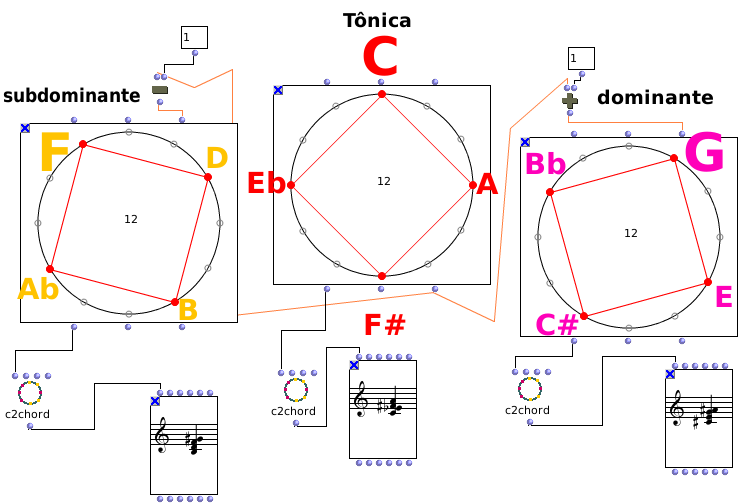
\includegraphics[scale=0.45]{axis/axisOM.png}
	\end{center}
	\legend{Fonte: autor }
\end{figure}


Lendvai chama de \textit{"polo e contra-polo"}\ a relação entre os trítonos nas duas extremidades (que chama de "eixo primário") e observa que o eixo perpendicular (ou "eixo secundário") possui também sua relação de \textit{"polo e contra-polo"}\ entre o que seriam a relativa e a mediante de uma tônica pelo ciclo de quintas. 

A relação entre este \textit{"\textbf{sistema de eixos}"} portanto pode ser a de analogia ao movimento de passo \textit{"$subdominante \leftrightarrow tônica \leftrightarrow dominante$"}\ que se move por passos de 30 graus pelo ciclo de quintas original.  

A diferença é que neste caso a relação mais importante entre as notas do eixo não seria exatamente por um critério baseado na busca de notas comuns de acordes para servirem de pivôs para resoluções tonais ou da busca por notas sensíveis para a solução de dissonâncias por grau conjunto. E sim, uma questão de \textbf{"\textbf{parentesco funcional}"} das sonoridades \textbf{dos intervalos que giram de 90 em 90 graus dividindo simetricamente o total cromático numa soma de quatro intervalos de três semitons} (ver Figura 2). 

\begin{citacao}
É essencial perceber que os eixos em particular não devem ser considerados como acordes de sétima diminuta, mas como relações funcionais de de quatro diferentes tonalidades, o que pode ser bem comparado com as relações menor-maior da música clássica.\cite[p. 3]{lendvai1971bela}\footnote{
Is essential that the particular axes should not be considered as chords of diminished seventh, but as functional relationships of four diferent tonalities, which may best be compared to the minor-major relations of classical music.\cite[p. 3]{lendvai1971bela}}
\end{citacao}

As três transposições possíveis dos eixos de quatro notas tornam a transformação de \textit{"transposição do sistema de eixos"} \textbf{\textbf{\underline{geometricamente}}} similar ao movimento \textit{"$subdominante \leftrightarrow tônica \leftrightarrow dominante$"},\ mas nem sempre pelos mesmos critérios de uma harmonia tonal funcional, apesar de poder servir-se deste como estratégia de construção de ambiguidades politonais.

\begin{figure}[!h]
	\caption{\label{fig_grafico}Sistema de Eixos - Rotacão entre primário e secundário}
	\begin{center}
	    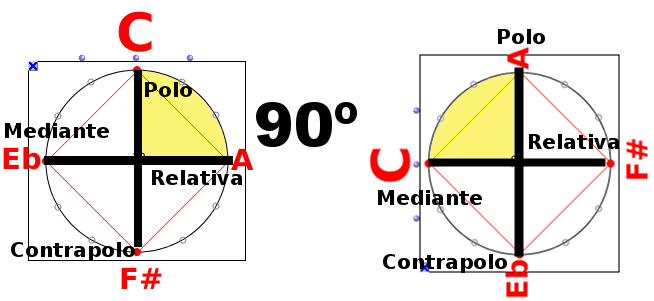
\includegraphics[scale=0.4]{axis/PoloContrapolo.png}
	\end{center}
	\legend{Fonte: autor }
\end{figure}


Lendvai toma este conceito de "polo e contrapolo"\ como \textit{\textbf{"uma das estratégias estruturais mais fundamentais na música de Béla Bartók"}}\cite[p. 04]{lendvai1971bela} e cita alguns exemplos que confirmam que este tipo de modulação era recorrente.

 %%%
Na \textit{"Sonata para dois pianos e Percussão"} o motivo inicial é transposto três vezes entre os dois pianos em sua relação de trítono \textit{"polo e contra-polo"} e nestas três entradas consecutivas deste motivo é apresentado com as três transposições possíveis do \textit{"sistema de eixos"}.

A relação \textit{polo $\leftrightarrow$ contra-polo} que pode ser observada nestas entradas, pode ser percebida como a analogia com o pêndulo \textit{"subdominante $\leftrightarrow$ tônica $\leftrightarrow$ dominante"} proposta por Lendvai: inicia com a relação motívica, destacando a relação $Dó \leftrightarrow Fá\sharp$ (compassos 2-5 / Figura 3), em seguida (compasso 8-9 / Figura 4) entra o eixo de $Sol \leftrightarrow Ré\flat$ - como se Sol surgisse de uma relação "dominante" derivada do Dó anterior (Figura 3), e Ré$\flat$ (ou seu enarmônico Dó$\sharp$) estivesse numa paralela relação "subdominante" similar com o Fá$\sharp$ do piano inicial. 

No compasso 12 (Figura 4) entrada do jogo de paralelismo entre os dois pianos com as transposições  $G \leftrightarrow Ré\flat$ e $Lá\flat \leftrightarrow Si$ é como se agora introduzissem "por rotação" do sistema de eixos proposto por Lendvai uma nova possibilidade de relação de modulação com as polarizações dos compassos anteriores. O que nos compassos iniciais foi a sequencia \textit{polo $\leftrightarrow$ contra-polo: $Dó \leftrightarrow e Fá\sharp$} agora acontece paralelamente com a transposição pelo eixo horizontal do sistema: a relação \textit{terça menor $\leftrightarrow$ sexta maior}.

\begin{figure}[!h]
	\caption{\label{fig_grafico}O plano melódico do motivo inicial de \textit{"Sonata para dois pianos e Percussão"}  parece ser o de fechar o total cromático com a transposição paralela da melodia nos dois pólos, fazendo um pólo para cada piano. }
	\begin{center}
	    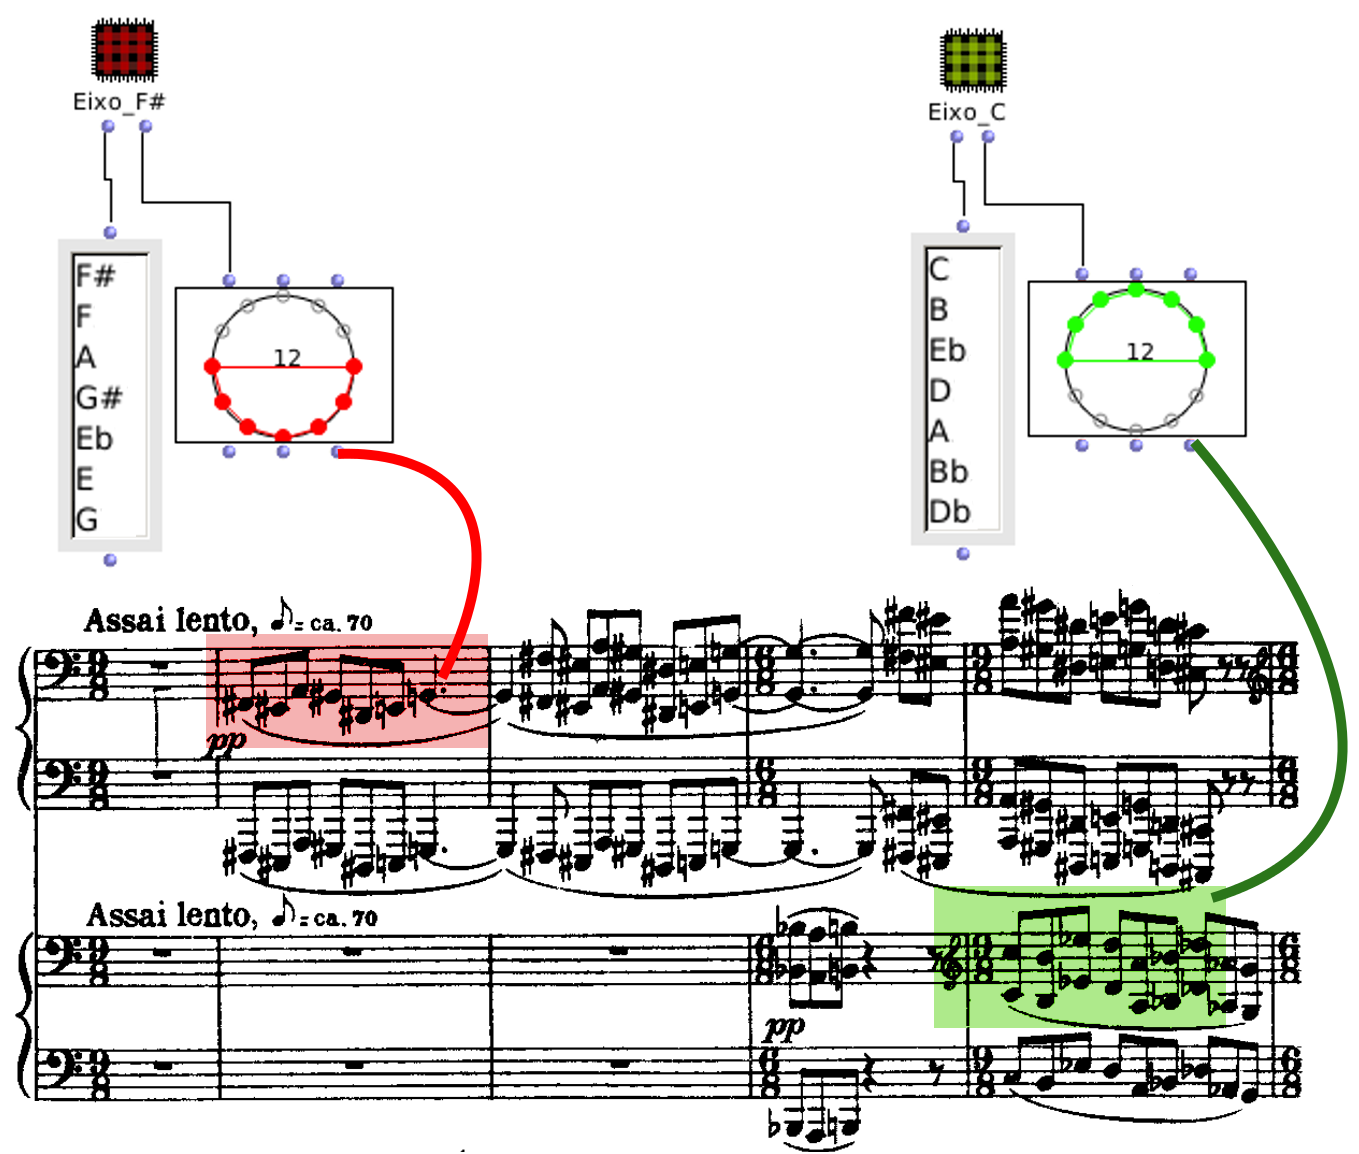
\includegraphics[scale=0.25]{axis/sonata2pianos_dofasus.png}
	\end{center}
	\legend{Fonte: autor }
\end{figure}



Podemos observar (Figura 3) que já nas entradas do motivo inicial temos uma estratégia de introdução de uma coleção de sete notas a partir de um polo (detalhes na Figura 5), e mais sete a partir do seu contrapolo em sua voz de resposta no segundo piano. 

As duas vozes juntas dividem o total cromático em dois, tendo como notas comuns as notas do eixo secundário do sistema de Lendvai (a mediante e a relativa: no caso de Fá$\sharp$ e Dó, por exemplo, as notas comuns são Lá e Mi$\flat$ ).

\begin{figure}[!h]
	\caption{\label{fig_grafico}Encadeamento dos eixos através das transposições do motivo inicial }
	\begin{center}
	    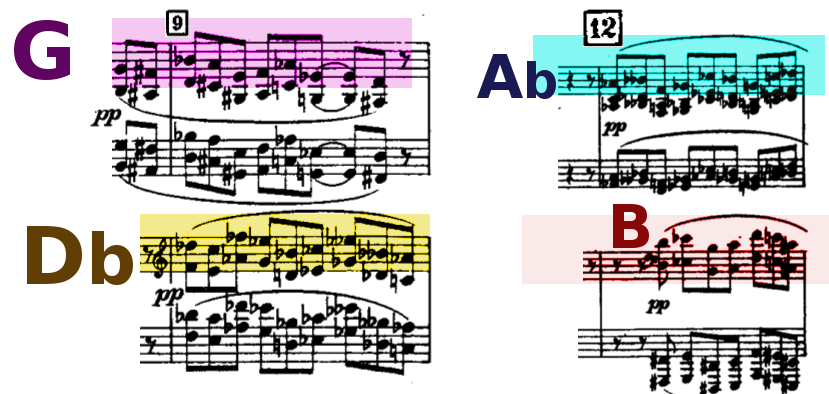
\includegraphics[scale=0.38]{axis/sonata2pianos_mm9-12.png}
	\end{center}
	\legend{Fonte: autor }
\end{figure}

É possível também inferir que a melodia tema sugere um giro em torno de um eixo que prolonga a expectativa do passo cromático $Fá\sharp \rightarrow Sol$ (e assim por diante em suas transposições - ver figura 5). 

O contorno possui uma simetria no núcleo interno de intervalos\footnote{"Um aglomerado simétrico de semitons equilibrados em torno de um eixo"\cite[p. 120]{straus2004}} com um segmento onde há um salto por quinta invertida no meio de duas células de passo cromático que estão distantes do inicio e do fim da melodia por um salto de 3 semitons (Figura 5). 

Esta estratégia composicional com simetrias internas\footnote{C.f. "Eixo de Inversão"\cite[p. 121]{straus2004}} recorrentes em Bartók por rotações de "células intervalares"\cite[p. 128]{susanni_antokoletz2012music} será comentadas na \autoref{simetria}.


\begin{figure}[!h]
	\caption{\label{fig_grafico}Possível estratégia composicional em nível melódico do motivo inicial de \textit{"Sonata para dois pianos e Percussão"}}
	\begin{center}
	    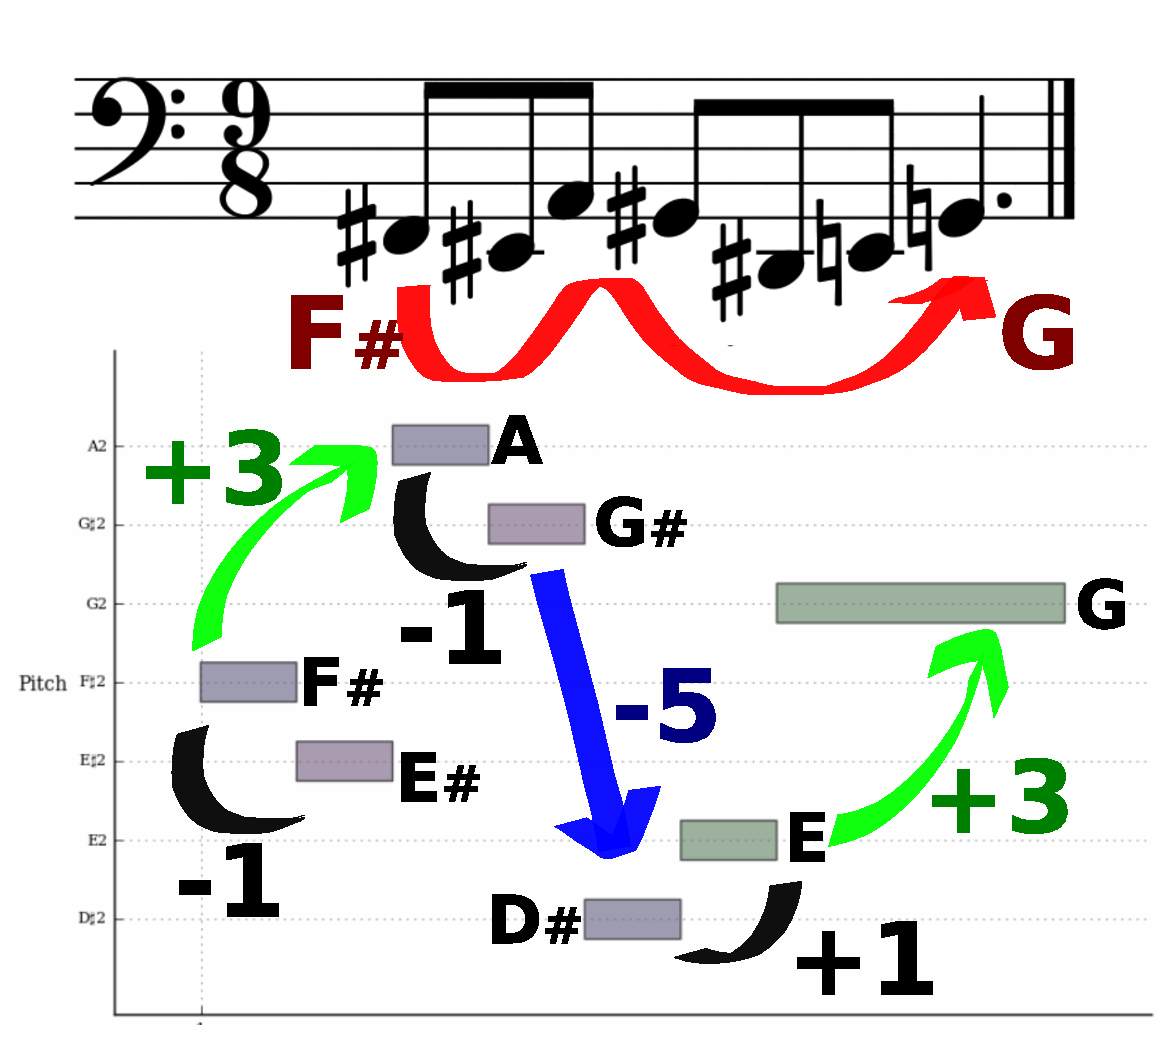
\includegraphics[scale=0.4]{axis/temasonata2P.pdf}
	\end{center}
	\legend{Fonte: autor }
\end{figure}


Lembremos também que as transposições em 3 semitons sugerem esta equivalência de sonoridade das transposições pelo mesmo sistema de eixos usado nas transposições da melodia completa e que o salto em quinta invertida no meio do segmento remete ao ciclo de dominantes tradicionalmente usado para modulações tonais.


\citeonline[p. 4]{lendvai1971bela} também aponta situações onde a estratégia de rotação dos polos do sistema de eixos é a conexão entre os movimentos de formas completas, como na opera \textit{"Castelo de Barba Azul"} ($Fá\sharp \leftrightarrow  Dó \leftrightarrow Fá\sharp$) e na \textit{"Music for Strings, Percussion and Celesta" } (que altera cada movimento entre os pólos e contrapólos dos eixos primário $Fá\sharp \leftrightarrow  Dó \leftrightarrow Fá\sharp$ e secundário $Lá\sharp \leftrightarrow  Mi\flat \leftrightarrow Lá\sharp$).


\subsection{A elaboração de uma sonoridade mista maior-menor}
\label{lendvai_maior_menor}



\citeonline[p. 08]{lendvai1971bela} elabora sobre a assimilação do "sistema de eixos"\ na música ocidental como uma evolução natural da harmonia funcional:  

\begin{citacao}
Uma revisão na evolução do pensamento harmônico leva-nos a conclusão de que o nascimento de uma sistema de eixos foi uma necessidade histórica, representando a continuação lógica (e em certo sentido a completude) da música funcional européia.\cite[p. 08]{lendvai1971bela}\footnote{A survey of the evolution of harmonic thinking leds to the conclusion that the birth of the axis system was a historical necessity, representing the logical continuation (and in a certain sense the completion) of European functional music.\cite[p. 08]{lendvai1971bela}}
\end{citacao}


a) O ciclo de dominantes inicia-se como um sistema de eixos de cadência onde as regiões vizinhas aparecem apenas como função dominante e subdominante, sem modulação para outras tonalidades. 

\begin{figure}[!h]
	\caption{\label{fig_grafico}Primeiro estágio: dominante/subdominate}
	\begin{center}
	    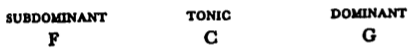
\includegraphics[scale=0.5]{axis/estagio01.png}
	\end{center}
	\legend{Fonte: \cite[p. 08]{lendvai1971bela} }
\end{figure}


b) O próximo passo é a introdução do eixo da tonalidade relativa (90 graus à esquerda do ponto da tonalidade). A modulação de tonalidade é induzida pela similaridade entre duas regiões diatônicas maiores e menores. Exemplo: Lá menor como relativa de Dó maior e vice-versa.

\begin{figure}[!h]
	\caption{\label{fig_grafico}Segundo estágio: modulação pela relativa}
	\begin{center}
	    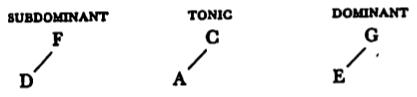
\includegraphics[scale=0.5]{axis/estagio02.png}
	\end{center}
	\legend{Fonte: \cite[p. 08]{lendvai1971bela} }
\end{figure}


c) No estágio mais avançado do romantismo é introduzido o jogo de ambiguidade entre a tonalidade maior e menor de um mesmo polo, permitindo que haja a estratégia de modulação pelo sistema de eixos tanto para 90 graus à esquerda (Ex: Lá menor e Dó maior) quanto 90 graus à direita (Ex: Dó menor e Mi bemol maior ).

\begin{figure}[!h]
	\caption{\label{fig_grafico}Terceiro estágio: modulação pela relativa com ambiguidade maior-menor em um dos polos }
	\begin{center}
	    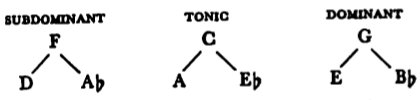
\includegraphics[scale=0.5]{axis/estagio03.png}
	\end{center}
	\legend{Fonte: \cite[p. 08]{lendvai1971bela} }
\end{figure}


d) Finalmente no último estágio onde é introduzida a politonalidade temos a assimilação da nota que está a 180 graus do polo (relação polo e contra-polo) pela sonoridade almejada de um modo misto "maior-menor"\ em quaisquer um dos pontos, desta maneira um giro completo:


\begin{figure}[!h]
	\caption{\label{fig_grafico}Quarto estágio: o jogo de rotação modulações por todos os polos do eixo }
	\begin{center}
	    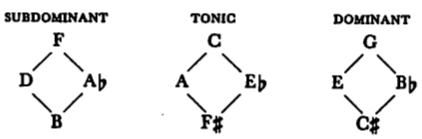
\includegraphics[scale=0.5]{axis/estagio04.png}
	\end{center}
	\legend{Fonte: \cite[p. 09]{lendvai1971bela} }
\end{figure}


Introduz-se assim a vertigem de uma sensação onde há uma teia de tonalidades simultâneas operando as expectativas de relações entre os três diferentes eixos. É como se cada um dos três ciclos de quatro terças menores também pudesse substituir por rotação a função de dominante ou subdominante que opera a tonalidade estrita, pois aqui operamos com uma expectativa ambígua. A função dominante de Dó, por exemplo, passa a poder ser substituída por qualquer nota do ciclo de Sol: Mi, Si$\flat$ ou Dó$\sharp$.

\begin{figure}[!h]
	\caption{\label{fig_grafico}Simultaneidade do modos maior-menor }
	\begin{center}
	    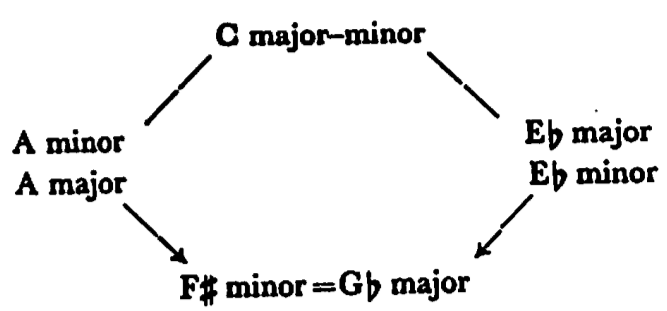
\includegraphics[scale=0.3]{axis/maiormenor.png}
	\end{center}
	\legend{Fonte: \cite[p. 10]{lendvai1971bela} }
\end{figure}

\citeonline[p. 10]{lendvai1971bela} atribui também a possibilidade de substituir-se Sol (a dominante de Dó) por Mi e Si$\flat$ a uma justificativa acústica de similaridade pela série harmônica, como veremos a seguir. 



\subsection{Especificidades da coleção acústica (overtone)}

\citeonline[p. 11]{lendvai1971bela} também procura  justificativa para o sistema de eixos na observação da sequência derivada da série harmônica. Sabemos que partindo de uma nota fundamental vibrando, teremos uma sequência de harmônicos derivados das suas subdivisões por números naturais - 1/2 , 1/3, 1/4, e assim por diante. Como podemos ver na figura abaixo:

\begin{figure}[!h]
	\caption{\label{fig_grafico}A série harmônica }
	\begin{center}
	    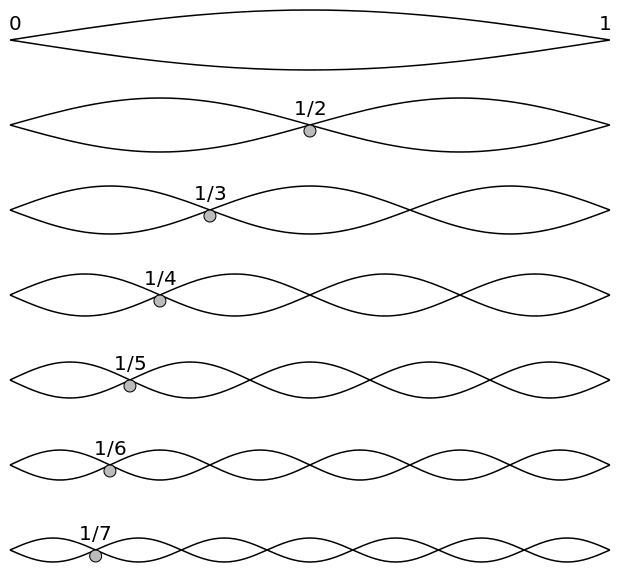
\includegraphics[scale=0.3]{axis/serie_harmonica.png}
	\end{center}
	\legend{Fonte: wikimedia.org }
\end{figure}

Considerando uma série acústica partindo de Dó no registro grave de 65.406Hz, podemos encontrar a série harmônica multiplicando esta frequência fundamental sucessivamente por 1,2,3,4 e assim por diante. Teremos oitavas em todos os números que são potência de dois: 2,4,8,16... Para os números intermediários ente estas oitavas encontraremos valores, que por aproximação, podem ser usados para gerar a sequência (partindo de Dó): [ Dó1, Dó2, Sol2, Dó3, Mi3, Sol3, Si$\flat$3, Dó4, Ré4, Mi4, F$\sharp$ 4, Sol4, Lá4, Si$\flat$4, Si4, Dó5, ...].

Lendvai pontua que, já que consideramos (na teoria tradicional) este primeiro harmônico que não é oitava (no caso de Dó, o Sol ) como chave para estabelecer as relações de dominante e sua inversão (a subdominante), podemos também tentar encontrar relações com estes próximos harmônicos - a terça maior e a sétima menor. Com isto encontra-se a sonoridade que justifica mais uma vez a expansão do sistema de eixos.

Lendvai propõe a observação das relações destes dois sobretons, a terça e a sétima, e demonstra assim que ambas terão como primeiros harmônicos (fora a oitava e a quinta justa) os harmônicos Sol$\sharp$/La$\flat$  e Ré, apenas em posições invertidas (o quinto e o sétimo harmônico e vice-versa).

Interessante então notar que estes dois harmônicos (Mi e La$\flat$) terão como seus próprios harmônicos as notas Dó e Fá$\sharp$/Sol$\flat$, também apenas em posições trocadas. Isto é, esta relação retorna para o eixo de polo e contra-polo de Do$\leftrightarrow$Fá$\sharp$. Podemos observar esta relação na figura 12.
 

\begin{figure}[!h]
	\caption{\label{fig_grafico}A série harmônica }
	\begin{center}
	    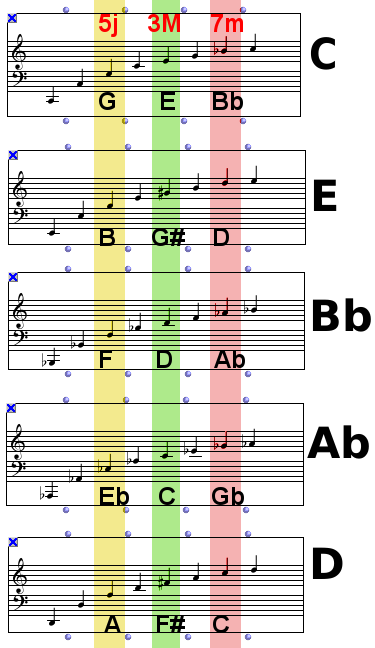
\includegraphics[scale=0.65]{axis/eixo_acustico.png}
	\end{center}
	\legend{Fonte: autor }
\end{figure}

Considerando esta propriedade, Lendvai sugere que na música de Bartok isso possibilita a substituição de dominantes ou subdominantes pelo giro dos eixos - permitindo levar também em conta a relação 6m$\leftrightarrow$ T $\leftrightarrow$ 3M como uma relação de função similar à relação subdominante $\leftrightarrow$ tônica $\leftrightarrow$ dominante. 

Toma para isso em consideração que assim como \textbf{Dó é a \textit{"dominante da subdominante"}\ Fá} e o \textbf{Sol (harmônico de Dó) é também sua dominante}. A sonoridade induz essa proporcionalidade em relação ao harmônico Mi, que tem como seu terceiro harmônico o Lá$\flat$ .\cite[p. 11]{lendvai1971bela}.

\begin{figure}[!h]
	\caption{\label{fig_grafico}O giro de eixos que sugere equivalência nas relações de subdominante e dominante pela proximidade acústica da série harmônica. }
	\begin{center}
	    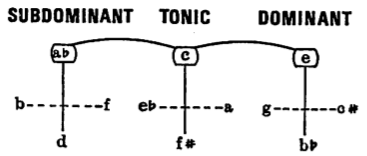
\includegraphics[scale=0.5]{axis/giro_de_eixos.png}
	\end{center}
	\legend{Fonte: \cite[p. 15]{lendvai1971bela} }
\end{figure}


\pagebreak
\subsection{Expectativas de grau sensível}

Outra observação interessante de Lendvai é sobre a resolução por grau sensível em Bartók. Considerando a possibilidade de trabalhar equivalências pelo giro do sistema de eixos, é possível também considerar a sonoridade da inversão da função sensível (ex: Fá $\leftrightarrow$Si).

A sonoridade de resolução de Si$\rightarrow$Dó no passo sensível V7 $\rightarrow$I pode então ser substituída pela cadência Fá  $\rightarrow$ Fá$\sharp$ com a função  V7 $\rightarrow$iv$\sharp$. Lendvai chama isto de \textit{"Pseudo-cadência bartokiana"}\cite[p. 13]{lendvai1971bela}

\begin{figure}[!h]
	\caption{\label{fig_grafico}\textit{"Pseudo-cadência bartokiana"} }
	\begin{center}
	    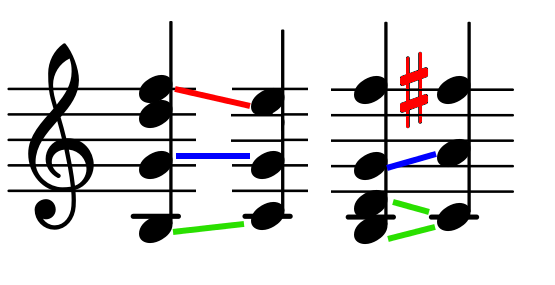
\includegraphics[scale=0.4]{axis/resolve.png}
	\end{center}
	\legend{Fonte: autor }
\end{figure}

Veremos mais algumas ideias sobre cadência, considerando a importância dos ciclos intervalares observados por \citeonline{antokoletz1984music}, na \autoref{ciclos}.


%%%%%%%%%%%%%%%%%%%%%%%%%%%%%%%%% ideias
%Polymode  Lydian-Mixolydian
%\cite{suchoff2004bartok}
%reflexo de imitação - mikrokosmos 29
%Substituição da cadência G7 -> C maior pela possibilidade G7->F\# maior-menor (desenhar as setas)
%\subsection{Tensões contrapostas de subdominante e dominante}
%\subsection{Dualidade entre os princípios de tonalidade e distância}
%Tríade aumentada C - E - Ab -> "surgindo" da mudança de função "subdominante-tonica-dominante" por uma rotação dos eixos laterais:(de G pra E e de F para Ab )
%%%%%%%%%%%%%%%%%%%%%%%%%%%%%%%%%%%%%%%%%%%%%%%%%%%%%%%%%%%%%%%%%%%%




\subsection{Secção Áurea e Fibonacci}
\label{fibo}

A secção áurea pode ser definida de diversas maneiras, dependendo da precisão que se está buscando na proporção. Para efeito de entendimento geométrico, podemos simplificar a dedução das fórmulas a partir da Figura abaixo: 

\begin{figure}[!h]
	\caption{\label{fig_grafico}Razão geométrica da proporção áurea }
	\begin{center}
	    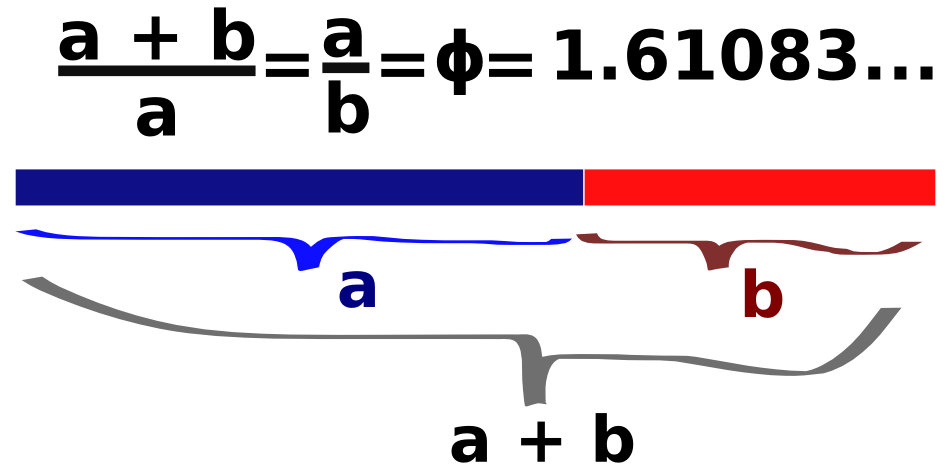
\includegraphics[scale=0.25]{axis/proportionaurea.png}
	\end{center}
	\legend{Fonte: autor }
\end{figure}	


Considerando no exemplo geométrico uma indução onde $(a+b)$ fosse igual a $\Phi$, teríamos então que ter a=1, pois $(a+b)/a$ também deve ser igual a $\Phi$ (que pode ser fixado em uma constante  $ \approx 1.61034... $ ) 

Logo, se sabemos que $(a+b)/a = a/b $, portanto $\Phi/1 = 1/b$, podemos também deduzir que $b = 1/\Phi \approx 0.61034.. $ 

Concluímos que: se a = 1, teremos $b \approx 0.61034 $. Se a=2, $b \approx 0.61034 \textbf{* 2} $ - e assim por diante.

Ou seja, \textbf{podemos obter a menor secção (b) fazendo a multiplicação da constante 0.61034 pelo valor de (a).}

A série de Fibonnaci é um caso especial de relação com a proporção áurea - multiplicando qualquer número da série pela constante $1/\Phi$ obtemos um número aproximado ao número anterior da série.

Para calcular a série de Fibonnaci seguimos a fórmula recursiva: adicionar os dois últimos números criando o próximo número da série. Se por exemplo começarmos com a sequência [1, 1], teremos como próximo número o 2 (1+1), o próximo será 3 (2+1), o seguinte 5 (3+2), e então 8, 13... e assim por diante. 

Na figura abaixo demonstramos a fórmula para encontrar a constante $1/\Phi$ e sua relação com a série de Fibonacci.

\begin{figure}[!h]
	\caption{\label{fig_grafico}A fórmula para encontrar a constante $1/\Phi$ e sua relação com a série de Fibonacci, testada no OpenMusic. }
	\begin{center}
	    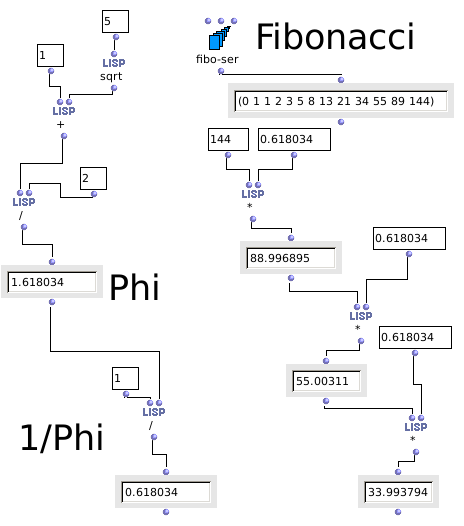
\includegraphics[scale=0.45]{OM_settheory/aurea.png}
	\end{center}
	\legend{Fonte: autor }
\end{figure}	

\pagebreak
\subsubsection{Geometria da Macro-forma com analogias na Micro-forma}

Um dos apontamentos mais específicos de Lendvai é a de que a música de Bartók esta profundamente fundada no uso de geometrias derivadas da proporção áurea. 

Reconhecida como uma das fórmulas matemáticas capazes de demonstrar equilíbrio em formas que vão de espirais das conchas até as proporções do corpo humano, esta razão geométrica foi sempre muito usada nas artes visuais e arquitetura - e as teses de Lendvai serviram para mitificar a obra de Bartók como uma das mais obsessivas acerca desta proporção.

\citeonline[p. 175]{lendvai1962duality} argumenta que seria possível resumir todo o sistema composicional bartokiano em uma relação entre estas proporções. Fornece exemplos que vão da forma geral de uma composição até o microcosmo motívico de estratégias de eixos de simetria e escalas.


\begin{citacao}
A secção áurea não é menos significante na obra de Bartók como elemento constituinte na criação da forma, melodia e harmonia do que a harmonização sobre a série harmônica e construção de frases fechando oito ou quatro compassos no estilo clássico vienense.
Por exemplo, em um estudo inicial eu demonstrei que cada unidade de \textit{"Sonata para dois pianos e percussão"}\ desde o todo até as pequenas células, são divididos pela secção áurea.\cite[p. 175]{lendvai1962duality}\footnote{
Golden section is no longer less significant constituent element in Bartok's creation of form, melody and harmony than overtone harmonization and construction in periods embracing eight or four bars in the viennese classical style. For example, in a early study I demonstrated thar every unit of the \textit{"Sonata for two pianos and percussion"} from the whole work to the tinest cells, is divided according to the rule of the golden section.\cite[p. 175]{lendvai1962duality}}
\end{citacao}

No caso da \textit{"Sonata para dois pianos e percussão"} alguns apontamentos são facilmente verificáveis: a estrutura do primeiro movimento tem como forma total 443 compassos e a recapitulação está posicionada precisamente no compasso 274 (443 * 0.618).

Alguns apontamentos são ajustados a uma aproximação - iniciando o seccionamento por dentro da unidade: no movimento final da \textit{"Sonata para dois pianos e percussão"} há um primeiro seccionamento que divide partes A e B (compassos 27.5 até 43.5 total), e novamente um seccionamento da parte A que a divide no compasso 17 a parte A e parte A'. Este caso no entanto pede que haja um adiantamento da contagem do seccionamento inicial em meio compasso, devido ao atraso no início do tema no movimento.

A série de Fibonnaci é usada por Lendvai para apontar uma estrutura nas escolhas motívicas que se constituem por concatenamento de intervalos que geram âmbitos de articulação das melodias. Destaca sobretudo a sequência de intervalos [0,3,5,8] por possuírem internamente uma potência de construir sonoridades e rotações da pentatônica (a partir do passo de 2-3 semitons) que pode seguir como estratégia recursiva de passos dentro dos intervalos consequentes. Exemplo: entre 8 a 13, os 5 semitons podem estar posicionados como 2+3, entre 13 e 21 como 3+(2+3), e assim por diante.

\citeonline[p. 179]{lendvai1962duality} destaca também a relação de intervalos de 3, 5, 8 semitons como essenciais na formação do agregado \textit{"maior-menor"}, entendendo a relação como uma conjunção de dois empilhamentos possíveis: o acorde maior com a terça invertida + o acorde menor com a quinta invertida, como demonstrado na figura 17:

\begin{figure}[!h]
	\caption{\label{fig_grafico}Secção áurea no modo misto maior-menor.  }
	\begin{center}
	    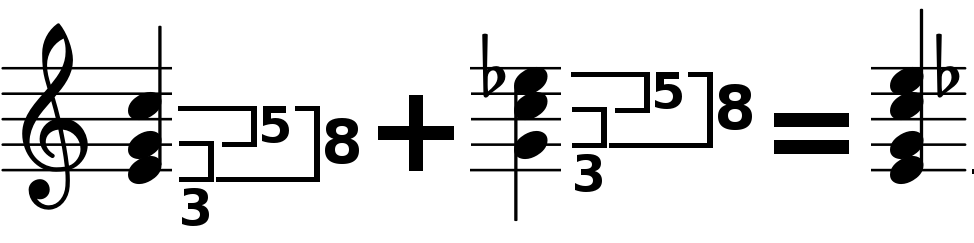
\includegraphics[scale=0.3]{axis/GS_maior_menor.png}
	\end{center}
	\legend{Fonte: autor }
\end{figure} 



\subsubsection{Críticas ao modelo de Lendvai}

Uma das principais críticas ao modelo de Lendvai, por \citeonline{karpati2006axis}, é a de \textbf{que sua escolha de intervalos e a demonstração de relações entre estes apresentam sonoridades arbitrárias,} já que potencialmente existem outros agrupamentos intervalares dentro da sequência que estariam fora da série de Fibonnaci (como os intervalos somados fora da ordem crescente 5+2 = 7 , 2+8 = 10 e assim por diante).

Por outro lado é interessante perceber que de fato Bartók estava consciente dessas estruturas de proporção áurea, considerando a visibilidade de suas decisões nas macroformas. Podemos entender também o modelo de Lendvai como a observação de recorrências "naturais"\ na geometria do material, como o apontamento de padrões espirais em conchas ou flores, um recorte de formas que sugerem equilíbrio.

Estes aspectos formais podem ser levados em conta para encontrar ideias que inspirem estrategias derivadas, mesmo sem a afirmação historicista de que havia uma consciência composicional total por trás de todas elas em seu apontamento original.


\section{Ciclos Intervalares}
\label{ciclos}

O conceito de ciclo intervalar, a partir da definição de \citeonline[p. 68]{antokoletz1984music} e conforme revisada por \citeonline[p. 22]{susanni_antokoletz2012music}, parte de uma identificação de ciclos de transposições possíveis de um determinado intervalo e sua inversão, dividindo a oitava em partes iguais.

O modelo é bastante intuitivo se tomado geometricamente como na figura 18:

\begin{figure}[!h]
	\caption{\label{fig_grafico}Alguns dos ciclos intervalares observados geometicamente em suas transposições no Open Music.  }
	\begin{center}
	    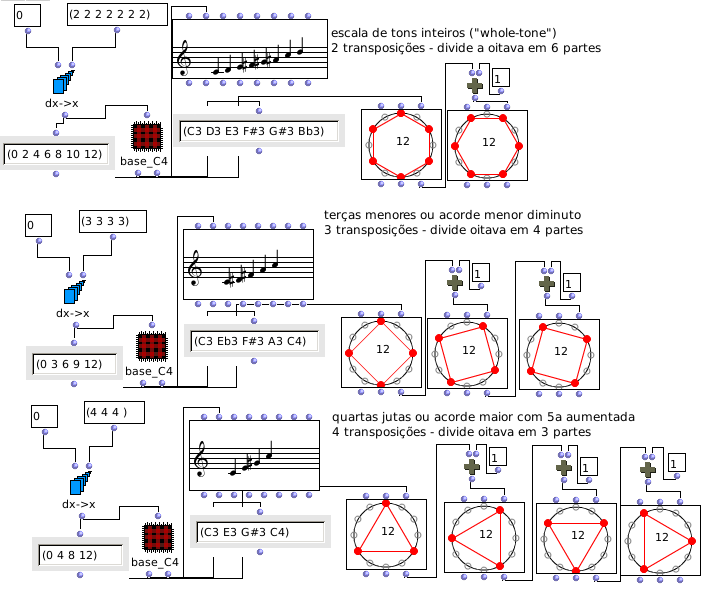
\includegraphics[scale=0.5]{ciclos/ciclosOM.png}
	\end{center}
	\legend{Fonte: autor }
\end{figure}

É possivel observar os seguintes ciclos simétricos:

\begin{itemize}
\item O intervalo de semitom divide a oitava no ciclo cromático de doze notas
\item O intervalo de tons inteiros produz duas transposições de seis notas
\item O intervalo de terças menores produz três transposições de quatro notas
\item O intervalo de terças maiores produz quatro transposições de três notas
\item O intervalo de trítono produz seis transposições de duas notas
\end{itemize}

Já a indução de um ciclo baseado no intervalo de quinta justa (ou sua inversão quarta justa), produz o que conhecemos pelo \textit{"ciclo de dominantes e subdominantes"}. É importante observar que por ser assimétrico este ciclo consegue gerar todo total cromático, mas não consegue percorrer apenas uma oitava sem quebrar o ciclo. Para chegar, por exemplo, de um Dó até outro, é necessário percorrer cinco oitavas num percurso ascendente por quartas justas, como podemos ver na figura 19.


\begin{figure}[!h]
	\caption{\label{fig_grafico}É necessário percorrer cinco oitavas girando pelas quartas justas para ir de C1 até C6  }
	\begin{center}
	    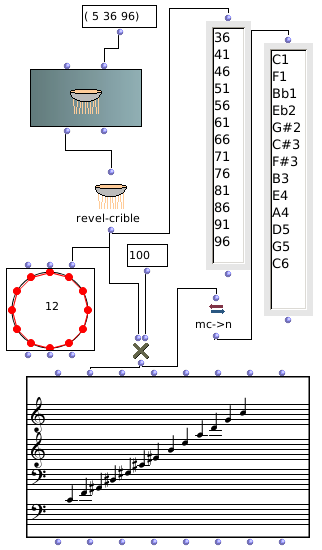
\includegraphics[scale=0.5]{ciclos/5JcrivosOM.png}
	\end{center}
	\legend{Fonte: autor }
\end{figure}

\citeonline[p. 23-25]{susanni_antokoletz2012music} destacam a importância motívica dos ciclos como estrategia de modulação entre os estados de equilíbrio que suspendem a sensação de tonalidade pela equidistância de seus intervalos. Exemplificam os casos de uso dos ciclos de terças maiores ou terças menores como geradores de acordes pivôs em potencial.

O caso do ciclo de terças menores é citado como matriz para a sonoridade de resolução por sensível em tríades vizinhas geradas a partir de cada uma das notas da tétrade do ciclo de terças menores. 


A figura 20 mostra a aplicação do apontamento em OpenMusic, para uso em composições.
 

\begin{figure}[!h]
	\caption{\label{fig_grafico}A resolução de uma coleção do ciclo de diminutas pela condução por nota sensível a um dos quatro acordes de resolução derivados   }
	\begin{center}
	    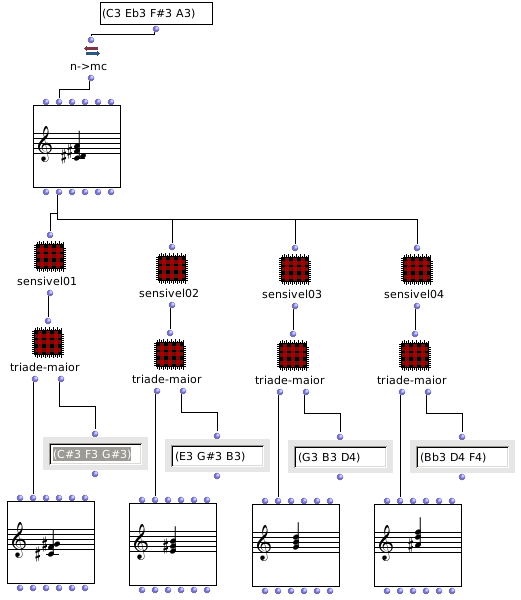
\includegraphics[scale=0.6]{ciclos/sensivel.png}
	\end{center}
	\legend{Fonte: autor }
\end{figure}

%inserir aqui resumo e comentários ssobre transformações do ciclo de terças menores e terças maiores exemplificados nos patches e explicados em \citeonline[p. 23-25]{susanni_antokoletz2012music}

Um segundo caso citado por \citeonline[p. 23-25]{susanni_antokoletz2012music} é o da construção de tétrades de dominante com sétima a partir de tétrades de um ciclo de terças menores, para então decidir o acorde de resolução. 

Neste caso uma das notas da tétrade original é aumentada em um semitom para tornar-se a quinta da tétrade dominante com sétima, para manter-se também como quinta do acorde final.


A figura 21 mostra aplicação desta transformação em um patch de OpenMusic.


\begin{figure}[!h]
	\caption{\label{fig_grafico}O ciclo de terças menores sendo usado para gerar uma dominante com sétima e sua resolução   }
	\begin{center}
	    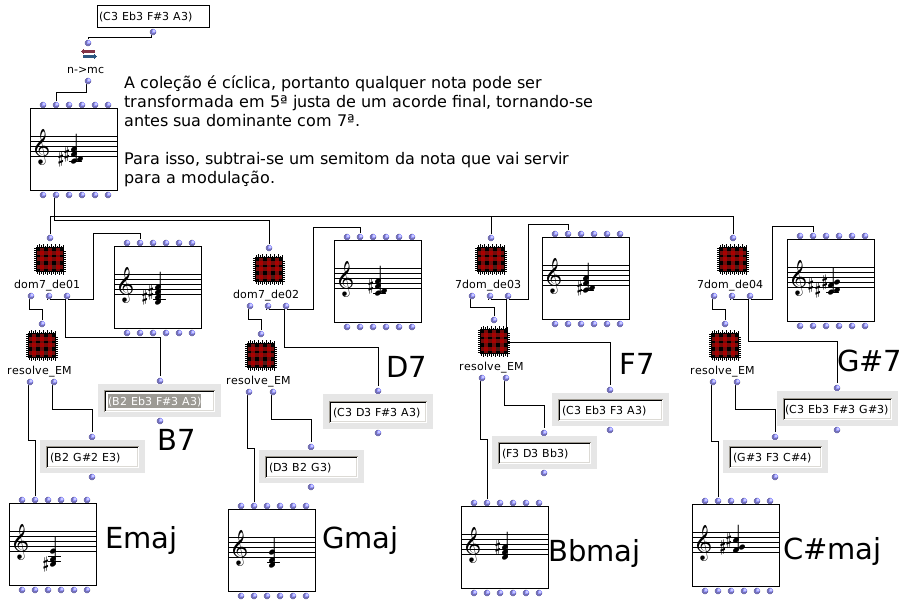
\includegraphics[scale=0.5]{ciclos/setimadominante.png}
	\end{center}
	\legend{Fonte: autor }
\end{figure}

O apontamento sobre o ciclo de terças aumentadas remete também à observação de Lendvai\footnote{ \autoref{lendvai_maior_menor} } sobre a assimilação completa da ambiguidade maior-menor e seu uso como sonoridade nos sistemas politonais ou pós-tonais. 

Como ferramenta para uso composicional e de análise e para efeito de demonstração deste apontamento, elaborei um script em music21 que gera todas as possibilidades de acordes próximos por aumento ou diminuição de um ou dois dos semitons da tríade aumentada original. \footnote{ver em \autoref{ciclotercas}.}

Na figura 22, um exemplo de 3 possibilidades onde o resultado são tríades maiores ou menores.

\begin{figure}[!h]
	\caption{\label{fig_grafico}A resolução de uma coleção do ciclo de terças maiores pela condução por nota sensível a um dos quatro acordes de resolução derivados. Detalhes sobre o script gerador no Apêndice.   }
	\begin{center}
	    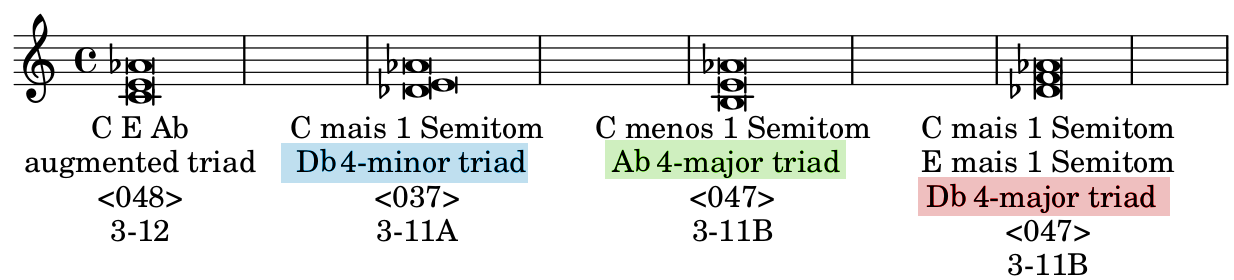
\includegraphics[scale=0.3]{ciclos/transpoe_triades_aumentadas.png}
	\end{center}
	\legend{Fonte: autor }
\end{figure}
\pagebreak



\section{Células de Altura de Antokoletz}
\label{celZ}

Elliot Antokoletz fundamenta boa parte de sua argumentação em seu livro \textit{"The music of Béla Bartók: a study of tonality and progression in twentieth-century music."}\cite{antokoletz1984music}, em torno da ideia de subdivisão da oitava em um complexo de ciclos intervalares rotacionados, operando identidades motívicas. 

Antokoletz destaca entre estes os grupos de intervalos que \textbf{chama "células X, Y e Z"}\cite[p. 69-77]{antokoletz1984music}. A nomenclatura de sua preferência - \textbf{"célula de alturas"}(\textit{"pitch cell"}) - é inspirada nos argumentos sobre transformações de grupos motívicos em composição serial propostos por George \citeonline{perle1981serial}. As definções das células X, Y e Z derivam dos estudos bartokianos de \citeonline{perle1955symmetrical} e Leo \citeonline{treitler1959}.

A definição de \textbf{célula X} é baseada em um \textbf{tetracorde cromático de semitons em sequência}, o que poderia ser reduzido a uma sequência prima de intervalos do tipo [0, 1, 2, 3]. 

No entanto é bom lembrar que esse conceito de células de altura é uma medida que pode ser relativizada por rotações ou permutações de relações entre os membros do grupo.

\citeonline[p. 131]{susanni_antokoletz2012music} exemplificam as relações entre os intervalos agrupando suas permutações em díades.

Se tomarmos por exemplo Dó como nota raiz (Dó, Dó$\sharp$, Ré, Mi$\flat$), teremos internamente as seguintes relações:


\begin{itemize}
\item Semitom: ( $Dó \rightarrow Dó\sharp$, $Dó\sharp \rightarrow Ré$, $Ré \rightarrow Mi\flat$ ) 

\item Tons Inteiros: ( $Dó \rightarrow Ré$, $Dó\sharp \rightarrow Mi\flat$ )

\item Terça menor: ( $Dó \rightarrow Mi\flat$ )
\end{itemize}

Ficam também implícitas as relações de inversão entre estas possibilidades.

\textbf{A célula Y é o tetracorde de tons inteiros} (que poderia ser reduzido a um forma prima [0, 2, 4, 6]). Da mesma maneira, \citeonline[p. 132]{susanni_antokoletz2012music} exemplificam as relações entre os intervalos, agrupando suas permutações em díades tomando o exemplo de Dó como nota raiz (Dó, Ré, Mi, Fá$\sharp$). 

Teremos assim internamente as seguintes relações:

\begin{itemize}
\item Tons Inteiros: ( $Dó \rightarrow Ré$, $Ré \rightarrow Mi$, $Mi \rightarrow Fá\sharp$ ) 

\item Terça maiores: ( $Dó \rightarrow Mi$, $Ré \rightarrow Fá\sharp$ )

\item Quarta aumentada / Quinta diminuta: ( $Dó \rightarrow Fá\sharp$ )
\end{itemize}


Já é definição de célula Z é bastante singular, porém é considerada aqui devido a relevância da obra de Antokoletz na literatura bartokiana norte-americana. 

A similaridade da célula Z com as anteriores é o fato de que sua construção permite que seja observada como uma pilha simétrica de intervalos. Por exemplo, a estrutura prima [ 0, 1, 6, 7] de uma célula Z possui dentro da distância de 0 a 7 semitons as distâncias simétricas respectivas de [1, 5, 1] de intervalos de semitom. 

No entanto, diferente das estruturas X e Y que são respectivamente pilhas de sequências imediatas de semitons ou tons inteiros (e que perderiam sua simetria em suas rotações) a célula Z possui, por causa de seu trítono, uma rotação onde permanece com a mesma estrutura intervalar: a rotação [ 6, 7, 0, 1 ]. 

\citeonline[p. 133]{susanni_antokoletz2012music} \textbf{definem a célula Z como o entrelaçamento de dois intervalos de quarta justa distantes por um semitom.} 

Por exemplo [ C, F, F\#, B] teria a nomenclatura \textbf{Z0/6} por ser composto da união das díades a partir das classes de altura 0 e 6. 

Podemos observar as permutações de díades na célula \textbf{Z0/6} a partir deste exemplo:

\begin{itemize}
\item Quartas Justas: ( $Dó \rightarrow Fá$, $Fá\sharp \rightarrow Si$) 

\item Trítonos: ( $Dó \rightarrow Fá\sharp$, $Fá \rightarrow Si$ )

\item Semitons: ( $Dó \rightarrow Si$, $Fá \rightarrow Fá\sharp$)
\end{itemize}


A nomenclatura \textbf{"Z(raiz/trítono)"} sugere uma maneira de construção da célula e destaca suas duas rotações que possuem um âmbito de 11 semitons. 

O principal problema das nomenclaturas de \textit{"células de alturas"}\ de Antokoletz é que elas não são muito adotadas fora do contexto das análises de Bartók.

O termo \textit{"conjunto Z"},\ por exemplo, tem um sentido totalmente diferente\footnote{ver \autoref{pos_tonal} } dentro da nomenclatura da  \textit{"Teoria dos conjuntos de classes de altura"}\footnote{Doravante também referida aqui pela sigla T.C.C.A}\ de Allen \citeonline{forte1973structure}. \citeonline{susanni_antokoletz2012music} negam-se ao uso da nomenclatura padronizada pela \textit{"Teoria dos conjuntos das classes de altura"}\ por considerá-la "alienante".\footnote{c.f. \citeonline[p. xiii]{susanni_antokoletz2012music}} Esta idiossincrasia dificulta comparações com outros contextos.

Vale também lembrar que \cite[p. 51]{lendvai1971bela} também cita a célula Z, mas a denomina \textit{"modelo 1:5"}\ por possuir uma sequência de intervalos de 1 semitom seguido de 5 semitons.\footnote{Esta denominação também faz parte da busca de Lendvai por formas derivadas da secção áurea já discutidas na \autoref{fibo} . Ele cita também o uso de intervalos de 1:2 (escala octatônica) e de 1:3 (um semitom inteercalado com uma terça menor) } 

\begin{figure}[!h]
	\caption{\label{fig_grafico}Algumas evidencias da célula Z de Antokoletz nos Mikrokosmos, destacadas por Lendvai com o nome de "modelo 1:5". }
	\begin{center}
	    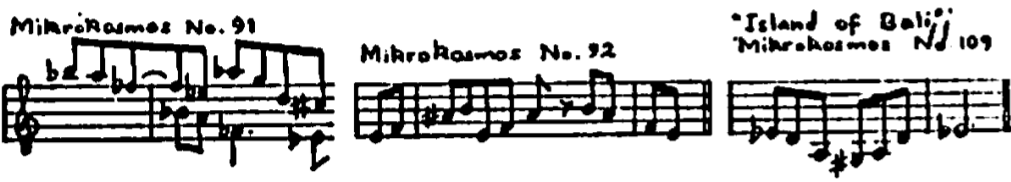
\includegraphics[scale=0.4]{intervalar/Lendvai_p52_ZCell.png}
	\end{center}
	\legend{Fonte: \cite[p. 52]{lendvai1971bela} }
\end{figure}

É importante destacarmos que a análise ganhará mais abrangência e suporte para comparações com outras análises pós-tonais com o uso da já consagrada nomenclatura de Forte. Veremos na \autoref{octa} um exemplo na proposta de Richard \citeonline{cohn1991bartok}. 
 
\section{Simetria Inversiva}
\label{simetria}

\citeonline[p. 72-77]{antokoletz1984music} define a ideia de simetria imersiva como uma estratégia composicional onde uma nota ou duas notas separadas apenas por um semitom de distância servem de eixo na definição de díades que serão intervalos simétricos a este eixo.

\begin{citacao}

Cada tetracorde simétrico pode ser analisado em partições de \textbf{díades de uma mesma soma.} Esta soma de díades vai formar parte de uma série de díades relacionadas simetricamente geradas pelo alinhamento de dois ciclos semitonais complementares. O eixo de simetria é expresso pela soma das classes de altura em qualquer díade.\cite[p. 72]{antokoletz1984music}\footnote{Any symmetrical tetrachord can be analyzed into\textbf{ dyads that have the same sum.} These sum dyads will form part of a series of symmetrically related dyads generated by aligning two inversionally complementary semitonal cycles. The axis of symmetry is expressed by the sum of the two pitch class numbers in any dyad.\cite[p. 72, grifo nosso]{antokoletz1984music}}
\end{citacao}

O que Antokoletz chama de \textbf{"díades de mesma soma"} é na verdade seu método para definir os pontos de simetria para uma díade qualquer. Toda díade terá dois eixos possíveis de simetria - um eixo que tem como ponto central \textbf{a metade da soma das duas classes da díade,} e outro igual \textbf{a este número mais seu trítono (ou seja: mais 6 semitons)}. 

Por exemplo: tomando a díade \textbf{Mi} $\leftrightarrow $ \textbf{Dó}, pegamos seus números de classe de altura [4, 0] e somamos, obtendo o valor 4 que dividido por 2 nos fornece \textbf{o valor 2, equivalente a nota Ré.} O segundo eixo seria o trítono de Ré, ou seja, 2 + 6 =\textbf{ 8, que é a classe de altura Lá$\flat$/Sol$\sharp$ }. 


\citeonline[p. 72-74]{antokoletz1984music} define como "díades de soma par"\ estes eixos onde os intervalos estarão em uma relação intervalar par com o eixo.

\textbf{Uma boa indução para enxergar intuitivamente a simetria} é pegar alguns exemplos de eixo onde a simetria fica visível no layout do piano.\footnote{No entanto, é bom lembrar que o conceito de eixo de simetria \textbf{não é dependente  da simetria visual do piano}, podendo ser transposto para cada uma das doze notas.}

No piano um eixo onde esta simetria de soma par fica visualmente explícita é o eixo em torno da altura \textbf{Lá$\flat$/Sol$\sharp$} (Figura abaixo).

\begin{figure}[!h]
	\caption{\label{fig_grafico}Simetria inversiva par}
	\begin{center}
	    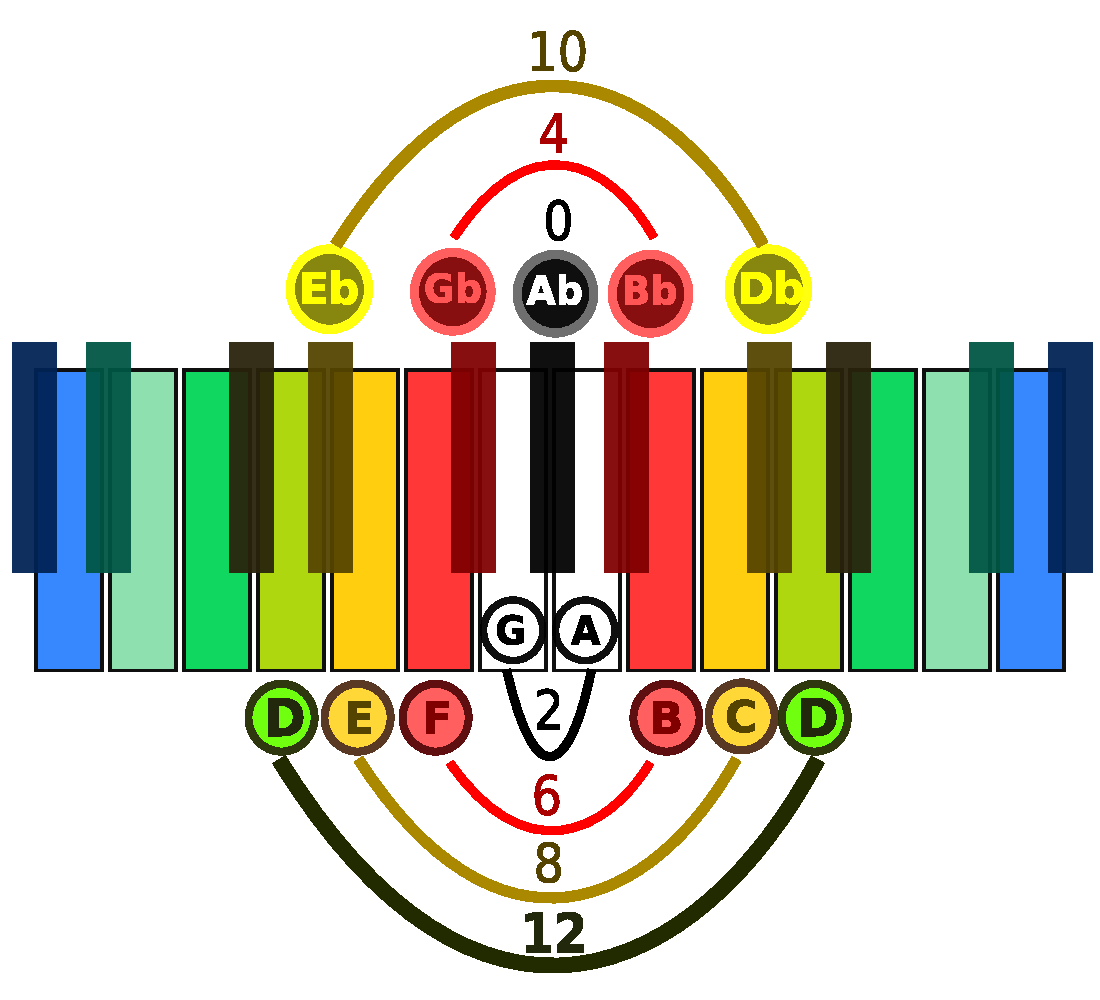
\includegraphics[scale=0.3]{axis/simetriainversiva_par.pdf}
	\end{center}
	\legend{Fonte: autor }
\end{figure}

De maneira similar podemos ver no piano um eixo onde a simetria de soma ímpar fica visualmente explícita: o eixo em torno das alturas \textbf{Mi} $\leftrightarrow $  \textbf{Fá}(Figura abaixo).

\begin{figure}[!h]
	\caption{\label{fig_grafico}Simetria inversiva impar}
	\begin{center}
	    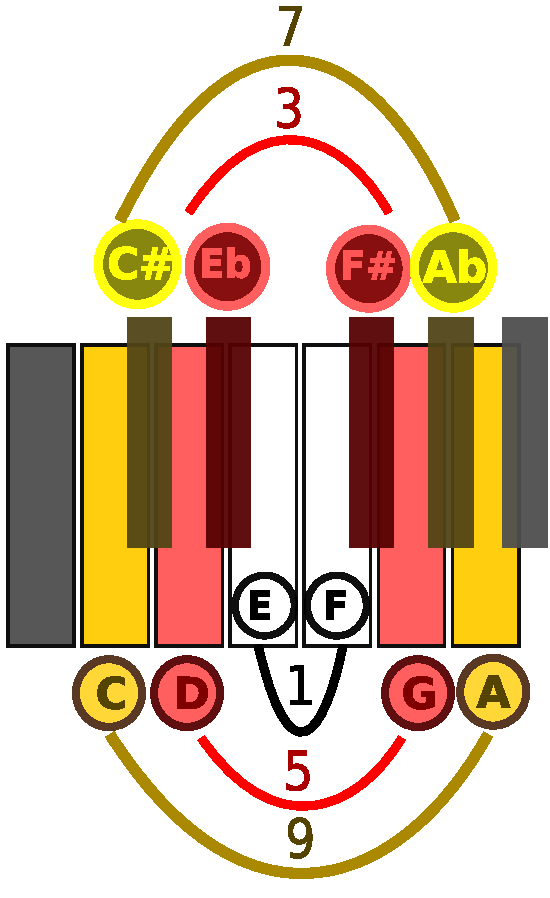
\includegraphics[scale=0.4]{axis/simetriainversiva_impar.pdf}
	\end{center}
	\legend{Fonte: autor }
\end{figure}

Se quisermos saber pelo método de \citeonline[p. 73]{antokoletz1984music} qual o eixo de simetria para a díade \textbf{Dó} $\leftrightarrow $ \textbf{Lá} pegamos seus números de classe de altura [0, 9] somamos e dividimos por 2, obtendo o valor \textbf{"quatro e meio"}. Aqui percebemos portanto que a soma ímpar precisa ser arredondada e para isso usa-se os dois semitons vizinhos, \textbf{as alturas 4 e 5, ou seja Mi e Fá (figura 25).} 
O outro eixo possível seria o par 4 e 5 \textbf{adicionados de seus trítonos: 10 e 11, ou seja, Si$\flat $ e Si.}

\subsection{Eixo de Simetrias como estratégia motívica}

Edward \citeonline{pearsall2004symmetry} observa na peça Mikrosmos 109 ("From the Island of Bali", já no motivo inicial, uma "célula germinativa"\ para outras transformações na peça; a construção simétrica esta presente tanto na construção do eixo [1,5,1] (Figura 15) quanto na construção uma escala completa de oito tons, que seria cortada ao meio por um intervalo ausente de Dó$\sharp$ (Figura 26).

\begin{figure}[!h]
	\caption{\label{fig_grafico}Exposição das primeiras citações do intervalo 151 e sua dissolução por rotações e inserção de novos intervalos. Código do script gerador no apêndice.}
	\begin{center}
	    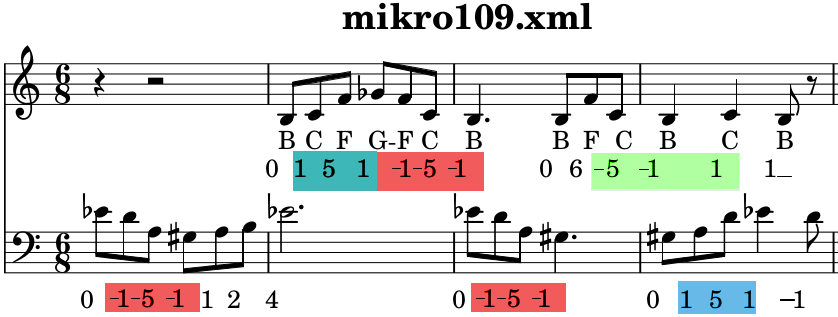
\includegraphics[scale=0.4]{estudosM21/contornoM109.png}
	\end{center}
	\legend{Fonte: autor }
\end{figure}

\begin{figure}[!h]
	\caption{\label{fig_grafico}Eixo de simetrias em torno de Dó$\sharp$ - estão presentes todas as díades do motivo inicial de Mikrokosmos 109 exceto a díade do trítono Mi-Si$\flat $ e a nota Dó$\sharp$}
	\begin{center}
	    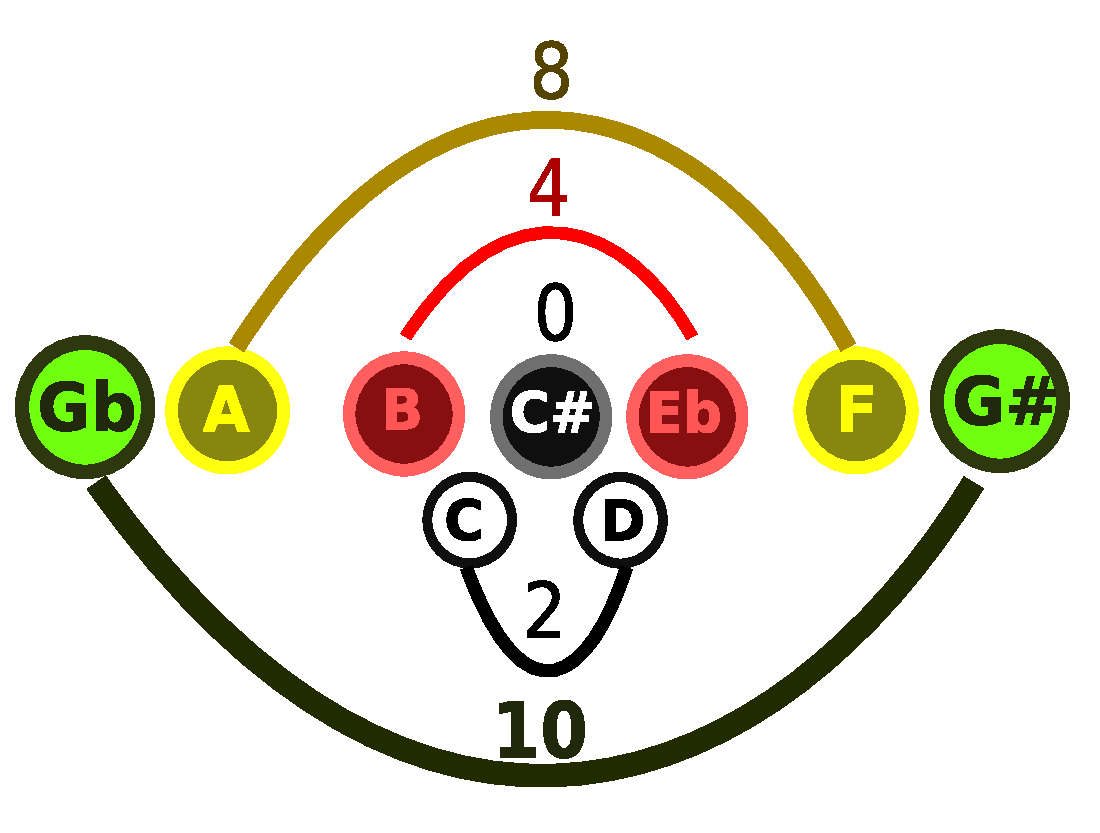
\includegraphics[scale=0.4]{axis/simetriamikro109.pdf}
	\end{center}
	\legend{Fonte: autor }
\end{figure}


\begin{citacao}
(...)O primeiro destes motivos esboça um contorno descendente 1/5/1. Este motivo que por si só representa uma estrutura simétrica no espaço das alturas - forma a base para uma série de transformações motívicas que se propagam mais adiante na peça.
O motivo da composição vira de ponta cabeça, aumentando o âmbito da composição e adicionando várias camadas novas. Tomadas juntas as duas coleções(...)formam uma oitava de escala octatônica. Esta escala simétrica (...) projeta uma série de intervalos de meio-tom acima e abaixo de Dó$\sharp$, o eixo de inversão.(...)\cite[p. 33]{pearsall2004symmetry}\footnote{(...)The first of these motives outlines a descent with the interval
succession 1 / 5/1. This motive - which itself represents a symmetrical structure in pitch space - forms the basis for a series of motivic transformations that propel the piece forward. (...)the motive turns
upside down, increasing the range of the composition and adding several new pitches. Taken together, the two pitch collections(...) form a one-octave octatonic scale. This symmetrical scale (...)
projects a 1/2 interval series above and below C$\sharp$, the axis of inversion.(...) \cite[p. 33]{pearsall2004symmetry}}
\end{citacao}

Richard \citeonline{cohn1988inversional} problematiza essa questão do arbítrio - sobre como estas transformações motívicas dos eixos de simetria poderiam tornar-se uma estratégia de escolha para as relações intervalares na obra de Bartók - para isso trabalha um conceito que chama "combinação transposicional". 

O argumento de Cohn é de que além da questão simétrica há uma prioridade decisória para encontrar situações onde o espelhamento dos segmentos também possua uma relação transpositiva que interesse ao plano de sonoridades da peça.

\citeonline[p. 25]{cohn1988inversional} aponta alguns conjuntos importantes na obra de Bartók (Figura 28) onde esta questão está presente. Retomaremos esta abordagem mais adiante, utilizando como exemplo a análise da importância da classificação e segmentação das coleções octatônicas presentes na peça Mikrokosmos 109.\cite{cohn1991bartok}

\begin{figure}[!h]
	\caption{\label{fig_grafico}Apontamentos de Cohn - Combinaçao Transposicional}
	\begin{center}
	    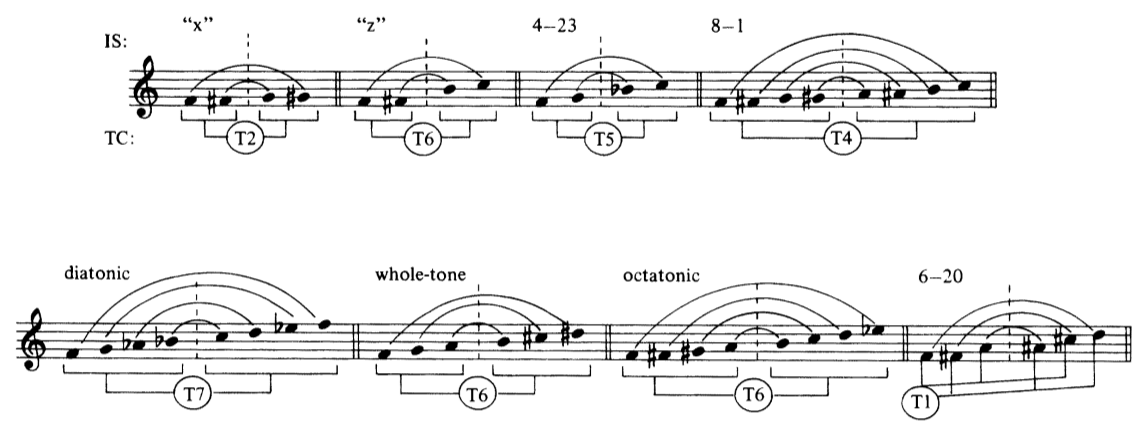
\includegraphics[scale=0.4]{axis/TCCohn.png}
	\end{center}
	\legend{Fonte: \cite{cohn1988inversional} }
\end{figure}



%\subsection{Centricidade por Equilíbrio Inversivo}
%%%%%
%\begin{citacao}
%Às vezes a idéia do equilíbrio inversivo em torno de um eixo pode afetar mais do que
%apenas um único conjunto de classe de notas ou grupo de conjuntos. Ela pode expandir-se
%para abranger todas as doze classes de notas. Nesse caso, cada classe de notas mapeia-se
%em outra (ou nela mesma) em torno de algum eixo. A Bagatela, Op. 6, No 2, de Bartók,
%começa com notas Láb e Sib repetidas na mão direita.
%
%Uma melodia começa no compasso 3 em Sin, um semitom acima da figura repetida, e
%então continua com Sol, um semitom abaixo da figura repetida. Depois vem Dó e Solb
%(dois semitons acima e abaixo), Réb e Fá (três semitons acima e abaixo), Ré e Fáb (quatro
%semitons acima e abaixo), e finalmente Mib, uma classe de notas que está cinco semitons
%tanto acima quanto abaixo. A única classe de notas que não foi ouvida é Lá, que está
%justamente no meio da figura repetida, um tipo de centro silencioso em torno do qual tudo
%se equilibra.
%\cite[p. 121]{straus2004}
%\end{citacao}



\subsection{Simetria Literal}
\label{simetrialiteral}


George Perle, apesar de também ter sido um entusiasta dos apontamentos motívicos em Bartók, alerta para o problema da definição de uma forma de macroestrutura não ser suficientemente determinada por estes achados de estratégias internas de construções simétricas:

\begin{citacao}
Por mais impressionantes que sejam estes procedimentos, deve ser observado que as formações simétricas em Bartók são apenas um aspecto incidental na totalidade de seus meios composicionais. Mesmo naqueles poucos trabalhos onde eles performatizam um papel estrutural significativo eles não definem o contexto em última instância, que é determinada ao invés disso por uma curiosa amálgama de vários elementos.
Poderiam as formações simétricas gerar uma estrutura musical total, assim como as relações triádicas tem feito tradicionalmente? As implicações do trabalho de Bartók sobre isto, assim como em outros aspectos mantém-se problemáticas. \cite[p. 300-312]{perle1955symmetrical} \footnote{Impressive as these procedures are, it must be observed that Bartk's symmetrical formations are only an incidental aspect of his total compositional means. Even in those few works where they perform a significant structural role they do not ultimately define the context, which is determined instead by a curious amalgam of various elements. Can symmetrical formations generate a total musical structure, as triadic relations have done traditionally? The implications of Bartók's work in this, as in other aspects, remain problematical.\cite[p. 300-312]{perle1955symmetrical}}
\end{citacao}

Como proposta para entender coerências macroestruturais para as simetrias na música de Bartók, Joseph \citeonline{bernard1986space} propõe a observação do que chama \textit{"simetria literal"}\ destacando a estratégia composicional por uma conjunção de simetrias intervalares que podem espalhar-se por todo âmbito de oitavas usado numa composição.  

Funciona como um  agregado sonoro que cria uma expectativa de equidistância de uma nota central em um grupo de intervalos - seja uma sequência de notas em forma melódica ou um cluster vertical. 

Por exemplo: { Db3, C4, B4} possuem entre si as distancias [-11, 0, 11 ] se considerarmos o C4 como um centro: todavia se usarmos o mesmo agrupamento dentro de uma única oitava [Db4, C4, B4], teremos as distâncias [ -1, 0, 11] onde - apesar de podermos considerar os intervalos [1,11] inversivamente equivalentes por inversão\footnote{Ver \autoref{pos_tonal}.} - não teremos a sonoridade de equidistância dentro de um eixo de 22 semitons. Planeja-se então uma equidistância que leve em conta todo âmbito de oitavas usadas na peça.

Bernard aponta escritos do próprio Bartók no ensaio "Problems of New Music" como evidência do procedimento. Bartók chamaria de \textit{\textbf{"simetria em espelho"}}.


\begin{figure}[!h]
	\caption{\label{fig_simetrialiteral} Alguns dos acordes de "simetria em espelho"\ apontados por Bartók e citados por \citeonline[p. 189]{bernard1986space}}
	\begin{center}
	    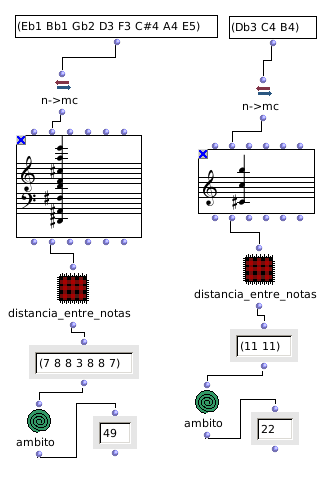
\includegraphics[scale=0.6]{axis/simetria_literal.png}
	\end{center}
	\legend{Fonte: autor }
\end{figure}


\section{Coleções referenciais ordenadas por conjuntos de classes de altura}

O uso sistemático de uma teoria unificada para a classificação de classes de altura em conjuntos relacionados por transposição, inversão, complemento, simetria e outras possíveis observações de propriedades específicas de agrupamentos intervalares tem a sua disposição a construção de alguns consensos que giram sobretudo em torno de uma área da musicologia de origem norte-americana\footnote{Sobre a influência da \textit{"Teoria dos Conjuntos de Classes de Altura"} norte-americana na musicologia européia ver \citeonline{aroundset2013}.} que tem se estruturado desde fortalecimento acadêmico do serialismo na segunda metade do século XX. Geralmente é referida como \textit{"Pitch Class Set Theory"}, e normalmente traduzida para português pelo termo \textit{"Teoria dos Conjuntos de Classes de Altura"} \cite{straus2004}.

\begin{citacao}
Foi, obviamente, Allen Forte quem foi o pioneiro das análises com a taxonomia dos \textbf{conjuntos de classes de alturas} aplicadas em conceitos da matemática, primeiro surgindo em tipos de Milton Babbit (a teoria conceitual), e em seguida com a inclusão e abstração de relações (como as relações de similaridade) construídas para uso analítico. A \textbf{"teoria de conjuntos"}\ de Forte (...) tem tido suas próprias ramificações e influência. Em particular, as próprias análises de Forte de peças individuais tem levado muitos outros a fazerem de maneira parecida, e a ideia inicial de Forte das relações de similaridade ( diferentes das relações de equivalência) sobre os grupos de classes de alturas tem visto florescer uma indústria teórica em torno disto, depois que os artigos seminais de Morris, Rahn  Lewin apareceram em 1980. \cite[p.  130]{rahn2004swerve}\footnote{
It was, of course, Allen Forte who in the USA pioneered the analytical with a taxonomy of pc-set application of concepts from mathematics, first arose also in serial Babbittian types (the concept theory), and following as some inclusion and with relations abstract up (such similarity relations) meant for analytical use. Forte's "set theory"\  (...) has had its own ramifications and influence. In particular, Forte's own analyses of individual pieces of music have led many others to do likewise, and Forte's initial idea of similarity relations (as distinct from equivalence relations) among pitch-class sets has seen a flourishing theoretical industry grow around it, after seminal articles by Morris, Rahn, and Lewin appeared in 1980. \cite[p.  130, grifo nossos]{rahn2004swerve}}
\end{citacao}

Para uma introdução resumida da terminologia da T.C.C.A., sugerimos a consulta do Apêndice do presente trabalho e dos patches de OpenMusic disponibilizados para sua demonstração. Para uma introdução mais aprofundada que serviu como referência aqui, sugerimos a tradução brasileira\footnote{O livro foi traduzido pelo professor Ricardo Bordini e publicado em 2013 pela editora EDUFBA\cite{strausBR2013}.} do livro de \citeonline{straus2004} e os trabalhos originais de \citeonline{forte1973structure} e \citeonline{rahn1980basic}.

\begin{citacao}

Bartók claramente favoreceu as quinze classes de tetracordes inversamente simétricas, em particular estas treze que foram capazes de serem deduzidas como conjuntos de classes de alturas com quatro notas simétricas (as duas exceções são 4-6 [0127] e 4-24 [0248]). Estas treze incluem  4-1 [0123], 4-21 [0246], e 4-9 [0167], que figuram de maneira proeminente nos escritos de Perle e Antokoletz, onde são chamadas células X,Y e Z; 4-17 [0347] o acorde "gamma" de Lendvai e 4-3 [0134] e 4-10 [0235], os tetracordes meio-octatônicos discutidos por Berry.\cite[p. 22]{cohn1988inversional}\footnote{
Bartók clearly favored the fifteen inversionally symmetric tetrachord-classes, in particular those thirteen which are capable of being realized as symmetric four note pitch-sets.
(The two exceptions are 4-6 [0127] and 4-24 [0248].) The thirteen include 4-1 [0123], 4-21 [0246], and 4-9 [0167], which figure prominently in the writings of Perle and Antokoletz, where they are called X, Y, and Z cells; 4-17 [0347], Lendvai's "gamma" chord; and 4-3 [0134] and 4-10 [0235], the half-octatonic tetrachords discussed by Berry.\cite[p. 22]{cohn1988inversional}}
\end{citacao}


\begin{figure}[!h]
	\caption{\label{fig_grafico} Simetrias em coleções referenciais citadas por Cohn}
	\begin{center}
	    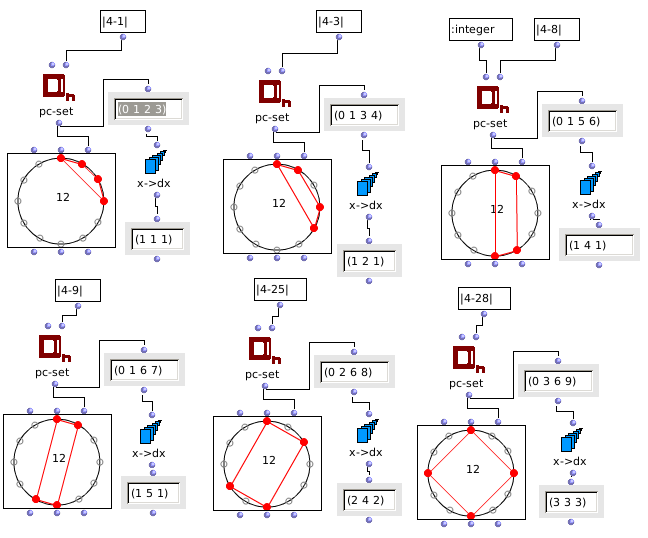
\includegraphics[scale=0.4]{axis/colecoes_simetricas.png}
	\end{center}
	\legend{Fonte: autor }
\end{figure}


Observamos a seguir um exemplo de análise de inspiração na T.C.C.A. que utiliza como base discussões sobre a coleção referencial octatônica - grupos de oito intervalos separados entre duas oitavas por uma sequência não-diatônica que intercala tom e semitom, gerando propriedades curiosas e de bastante uso na música de Bartók e no repertório pós-tonal em geral.


\subsection{Octatonismo e suas partições}
\label{octa}

Richard \citeonline{cohn1991bartok} propõe em seu artigo \textit{"Bartók's octatonic strategies: a motivic approach"}\ uma abordagem que utiliza a nomenclatura dos conjuntos de classes de altura propostas por Allen \citeonline{forte1973structure} na tentativa de construir um discurso sobre as coleções de sonoridades em Bartók que articule com uma continuidade das tradições analíticas.

Cohn aponta também a importância do conceito de simetria nestas estratégias composicionais:

\begin{citacao}
O presente estudo pretende demonstrar que a música de Bartok é mesmo baseada em tal sistema (simetria inversiva). As relações de alturas na música de Bartok é primariamente baseada nas subdivisões iguais da oitava em um total complexo de ciclos de intervalos. O conceito fundamental desta divisão igual é o da simetria.\cite{cohn1988inversional}\footnote{ The present study is intended to demonstrate that Bartok's music is indeed based on such a system. Pitch relations in Bartok's music are primarily based on the principle of equal subdivisions of the octave into the total complex of interval cycles. The fundamental concept underlying this equal-division system is that of symmetry. \cite{cohn1988inversional}}
\end{citacao}

Cohn no entanto destaca o que chama de "combinação transpositiva"\ como uma observação a ser tomada na escolha das coleções simétricas.

Considera importante sistematizar aspectos transpositivos, inversivos e relações intervalares com lastro na harmonia funcional. Para isso traça uma estratégia que parte do mapeamento de permutações da coleção octatônica, separando desta também derivações de díades e tétrades pelo que chama de "grau de fertilidade"\cite[p. 268]{cohn1991bartok} - a capacidade do segmento em relacionar-se por transposição com outros grupos de mesma cardinalidade (mesmo número de elementos).

Ao separar os grupos em pares relacionados por transposição, Cohn almeja encontrar um sistema de classificação de intervalos também por sua funcionalidade em parte da expectativa politonal que rege estas obras:

\begin{citacao}
Pares de notas são classificados tanto por classe de intervalo quanto classe de díade neste estudo. As duas classificações são idênticas, então a distinção é uma questão de orientação. Assim como com as classes de intervalo, os nomes das classes de díade correspondem ao seu menor intervalo, medido em semitons, disponível entre suas classes de altura constituintes. Assim entre as classes de díades eu incluo pares de alturas separados por meio tom, sétimas maiores, e seus equivalentes enarmônicos e compostos, e assim por diante até a classe de díades 6, o trítono. Apesar dos teóricos usarem a classe de intervalo mais frequentemente, o conceito de classe de díade permite uma comparação mais natural com conjuntos maiores.\cite[p. 265-266]{cohn1991bartok}\footnote{Pairs of notes are classified either by interval-class or by dyad-class in this study. The two classifications are identical, so their distinction is a matter of orientation. As with interval-classes, names of dyad-classes correspond to the smallest interval, measured in half-steps, available between their constituent pitch-classes. Thus dyad-class I includes pairs of pitches separated by half-step, major seventh, and their enharmonic equivalents and compounds; dyad-class 2 includes whole-steps, minor sevenths, and their enharmonic equivalents and compounds, and so forth up to dyad-class 6, the tritone. Although theorists use interval-class more frequently, the concept of dyad-class allows for a more natural comparison to larger sets. \cite[p. 265-266]{cohn1991bartok}}
\end{citacao}

A coleção octatônica é reconhecida como uma das importantes estratégias composicionais de construção motívica não-diatônica no repertório pós-tonal da primeira metade do século XX \cite{berger1963problems,antokoletz1984music,lester1989analytic,forte1991debussy,straus2004,de2013simetria}

O termo "coleção"\ é usado para diferenciar da ideia de "escala", onde fica implícita a importância motívica da ordem dos elementos. Há aqui também uma preocupação com propriedades adquiridas em rotação, segmentação, permutação, inversão, transposição ou qualquer transformação que derive de algum parentesco relevante com as coleções originais.

Vale  no entanto definir o conceito que funda a noção de octatonismo,\footnote{Allen \citeonline[p. 125]{forte1991debussy} cita o artigo de Arthur \citeonline{berger1963problems} como origem do conceito de octatonismo.} que é a alternância de tons e semitons dentro de uma oitava - gerando uma sequência de oito notas dentro deste âmbito. 

Sua forma prima é classificada como\textbf{ 8-28} na nomenclatura de \citeonline{forte1973structure}, possuindo os intervalos \textbf{[0, 1, 3, 4, 6, 7, 9, 10]}. \citeonline{straus2004} usa a nomenclatura  \textbf{OCT0,1}, indicando as duas alturas iniciais do conjunto: [0, 1].

\begin{figure}[!h]
	\caption{\label{fig_grafico} A coleção octatônica em sua rotação prima OCT0,1 e na sua rotação que inverte a ordem dos intervalos, normalizada para começar em OCT0,2}
	\begin{center}
	    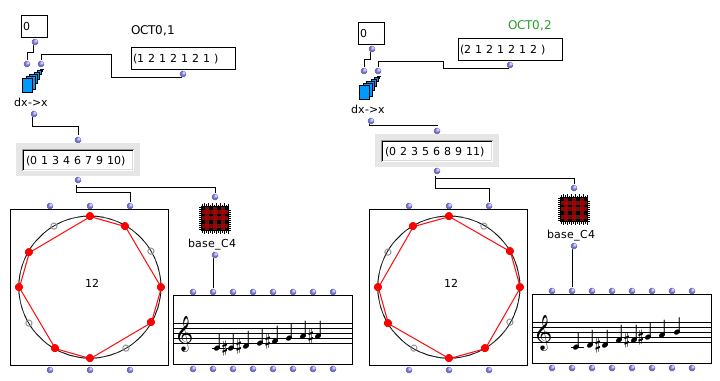
\includegraphics[scale=0.5]{octa/octaOM.png}
	\end{center}
	\legend{Fonte: autor }
\end{figure}

\citeonline{cohn1991bartok} propõe um formalismo sobre a permutação de díades e tétrades derivadas de coleções octatônicas para buscar em Bartók algumas estratégias composicionais enfatizando o que chama de \textbf{\textit{combinação transpositiva}} - "o procedimento geral de combinar entidades com suas próprias transposições". \cite[p. x]{cohn1991bartok}

Para isto \citeonline{cohn1991bartok} parte de uma série de definições para o particionamento das coleções em subgrupos:

\begin{itemize}
\item Os subgrupos não devem compartilhar elementos;
\item Subgrupos comparados devem possuir o mesmo número de elementos. 
\item As partições de uma nota só não serão analisadas pelo formalismo.
\item Tomando o exemplo da tétrade [C, E, G, B] - apenas interessam as permutações de díades relacionadas por transposição. Portanto a relação [C, B]$\leftrightarrow $ [E, G] não interessa, mas a relação [C, G]$\leftrightarrow $ [E, B], sim. No segundo caso temos um exemplo da transposição de uma relação de intervalo de quinta justa (7 semitons).
\item Um conjunto "fértil" tem pelo menos uma relação transposicional em suas permutações.
\item O "grau de fertilidade" na segmentação de tétrades em subgrupos de díades fica definido como o número de duplas de díades relacionadas por transposição que uma permutação entre os elementos pode gerar.
\item No caso da análise de segmentos octacordais o "grau de fertilidade"\ é medido na relação entre tétrades derivadas por permutações do segmento que tenham relação transpositiva. O "grau de potência"\ fica definido como as díades permutadas que possuam relação transpositiva entre si.

\end{itemize}

\begin{figure}[!h]
	\caption{\label{fig_grafico} Relações de combinação transpositiva. Note-se, por exemplo, que os conjuntos 4-9, 4-25 e 4-28 produzem três combinações transpositivas diferentes, teriam portanto \textbf{"grau de fertilidade"\ 3}, segundo a classificação de \citeonline{cohn1991bartok}  }
	\begin{center}
	    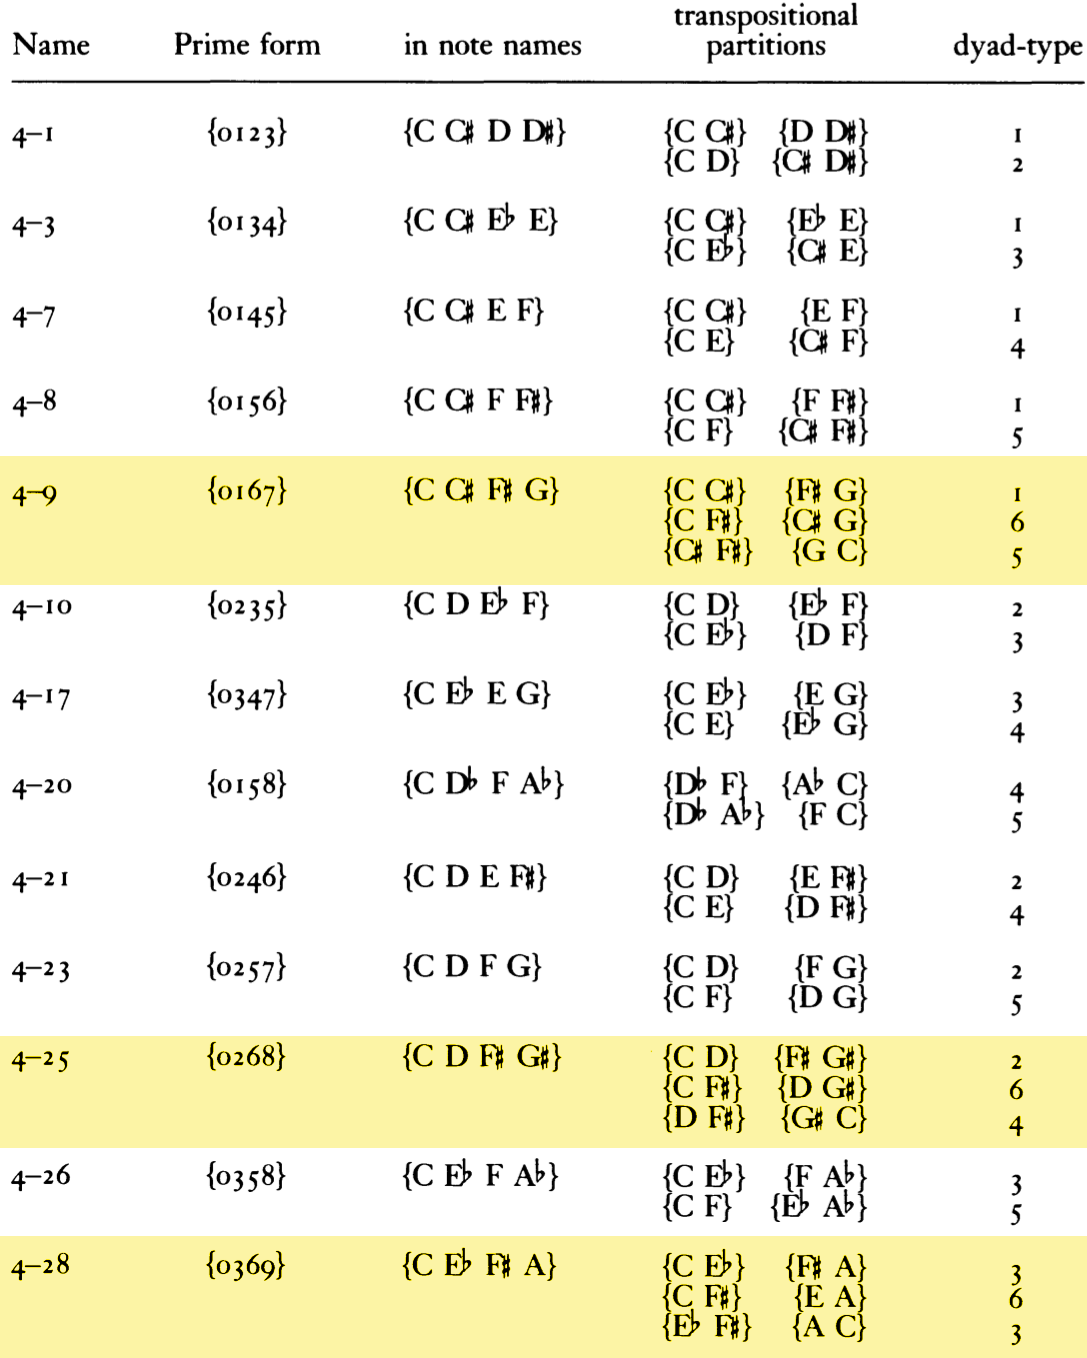
\includegraphics[scale=0.35]{octa/trasposiCohn.png}
	\end{center}
	\legend{Fonte: \cite{cohn1991bartok} }
\end{figure}


Baseado nestas regras, e fazendo um levantamento de octacordes com maior grau de \textit{"potência e fertilidade"}, \citeonline[p. 270]{cohn1991bartok} demonstra que a coleção octatônica (8-28) é a que mais se destaca, permitindo 11 ordenamentos em tétrades férteis e permitindo a partir destas 9 diferentes combinações transpositivas.


Organizando diferentes permutações de elementos de uma coleção octatônica em conjuntos de duas tétrades justapostas possível encontrar nelas todas relações transpositivas possíveis (de 1 a 6 semitons). \citeonline[p. 271]{cohn1991bartok} constrói uma tabela engenhosa para demonstrar estas permutações. 

Como exemplo, na figura 33 destaquei da tabela original de Cohn a permutação que gera a partir das duas tétrades do \textit{"conjunto Z de Antokoletz"}\footnote{ \autoref{celZ}} grupos de díades que possuem intervalos internos de 1, 5 ou 6 semitons .

A tabela também mapeia o retorno das díades para as tétrades, indicando em quais tétrades podemos encontrar aquelas díades.

\begin{figure}[!h]
	\caption{\label{fig_grafico} Tabela de grupos de tétrades derivadas da coleção octatônica e suas coleções de combinações transpositivas}
	\begin{center}
	    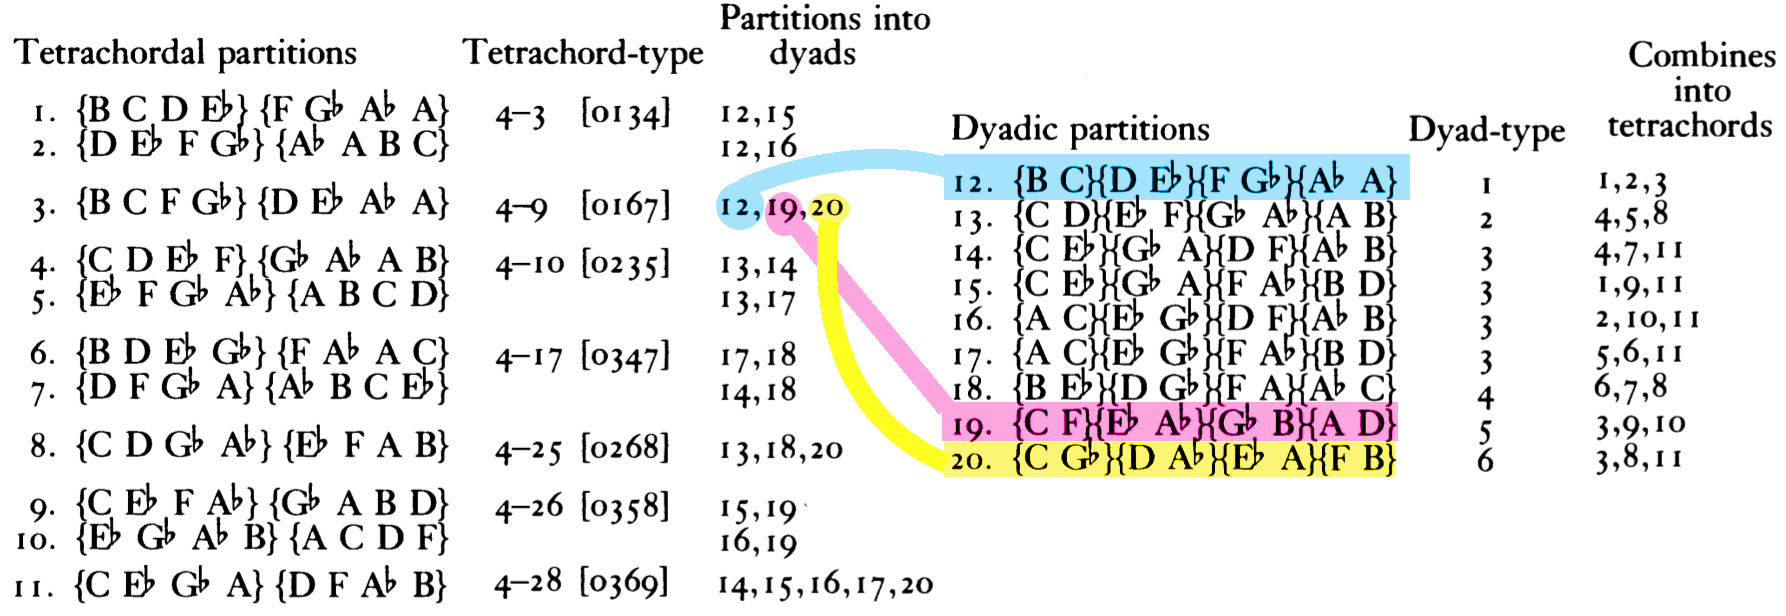
\includegraphics[scale=0.28]{octa/Tetrarelations03.png}
	\end{center}
	\legend{Fonte: \cite[ grifos nossos]{cohn1991bartok} }
\end{figure}

Cohn utiliza a reflexão sobre as combinações transpositivas para retirar alguns \textit{insights} em análises de estratégias octatônicas em Bartók. Destaco aqui da sua observação sobre a peça Mikrokosmos nº109 (\textit{"From de Island of Bali"}) o uso simultâneo de dois arranjos da coleção octatônica: a ordenação baseada na justaposição das células Z (intervalos 0, 1, 6, 7 semitons) e a inserção dos arranjos com a justaposição de tétrades da coleção nomeada por Forte como 4-26 - que é formata pela ordenação de distâncias em (0, 3, 5, 8)  semitons. 

Utilizei a sugestão de Cohn para construir dois patches de OpenMusic que fazem a redução das permutações possíveis das tétrades, organizando as díades em sua ordenação de menor para maior classe de alturas e permitindo a audição das sonoridades observadas - facilitando seu uso em procedimentos de composição derivados.

Na figura 34 demonstro as permutações da célula Z. Fica bastante intuitivo também observar no objeto de OpenMusic \textit{"n-cercle"} que a união dos dois conjuntos de tétrades pode formar uma octatônica.


\begin{figure}[!h]
	\caption{\label{fig_grafico} As permutações de díades internas a uma célula Z de Antokoletz, podem ser reduzidas a três coleções intervalares de 1, 5 ou 6 semitons (ou suas inversões). Este patch de OM mede as combinações transpositivas para qualquer tétrade permutada, podendo encontrar todas as relações da tabela de \citeonline[p. 271]{cohn1991bartok} }
	\begin{center}
	    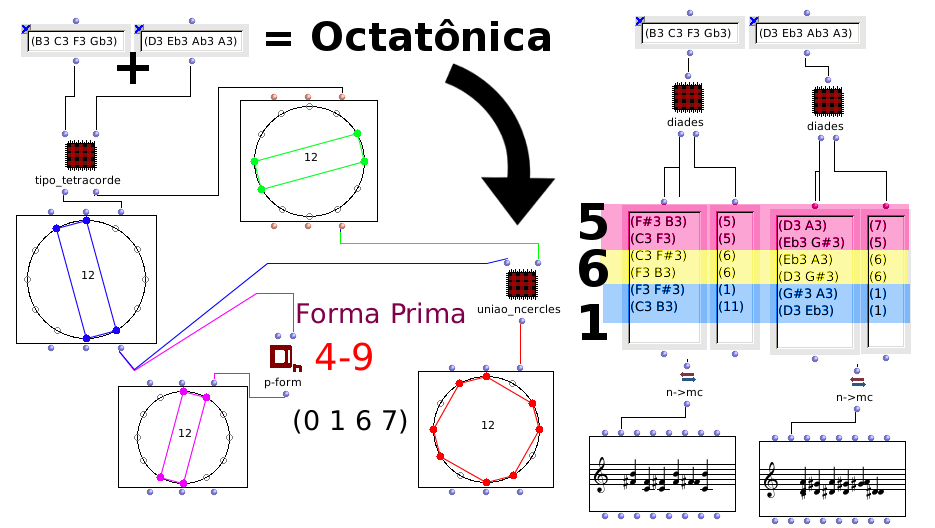
\includegraphics[scale=0.55]{octa/permutaCEL_Z.png}
	\end{center}
	\legend{Fonte: autor }
\end{figure}

Em \textit{Mikrokosmos 109} temos de maneira bastante destacada a sonoridade da célula Z de Antokoletz (coleção 4-9 de Forte), que se faz presente já na introdução do tema, de maneira predominante. Cohn sublinha no entanto o fato de que as "notas estranhas"\ a célula Z (circuladas na figura 35 com a letra X) são já citações para entrada da coleção 4-26, que é usada para destacar os intervalos de 3 e 5 semitons.

\begin{figure}[!h]
	\caption{\label{fig_grafico} Tétrade da coleção 4-26 citada no ínicio de Mikrokosmos 109. }
	\begin{center}
	    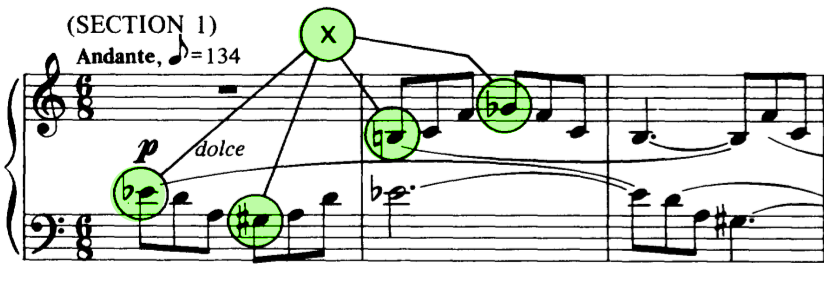
\includegraphics[scale=0.3]{octa/mikro_Bali01.png}
	\end{center}
	\legend{Fonte: autor }
\end{figure}

Os compassos finais da peça \textit{Mikrokosmos 109}\footnote{E sobretudo os acordes de resolução - ver figura 36} sequênciam que Bartók havia usado de fato o apontamento feito por Cohn: a justaposição das duas tétrades da coleção 4-26 formam uma coleção octatônica completa\footnote{Conferir na figura 37}, usada durante toda a composição como uma alternativa à permutação da octatônica formada pela justaposição de duas tétrades da coleção 4-9. 

\begin{figure}[!h]
	\caption{\label{fig_grafico} A conjunção das duas tétrades (X e Y) da coleção 4-26 formam uma segunda ordenação da coleção octatônica. Os acordes finais destacam a possibilidade de justaposição de X+Y. As notas Sol e Ré$\flat$ são as únicas que figuram fora das configurações octatônicas como ornamento entre as coleções motívicas.  }
	\begin{center}
	    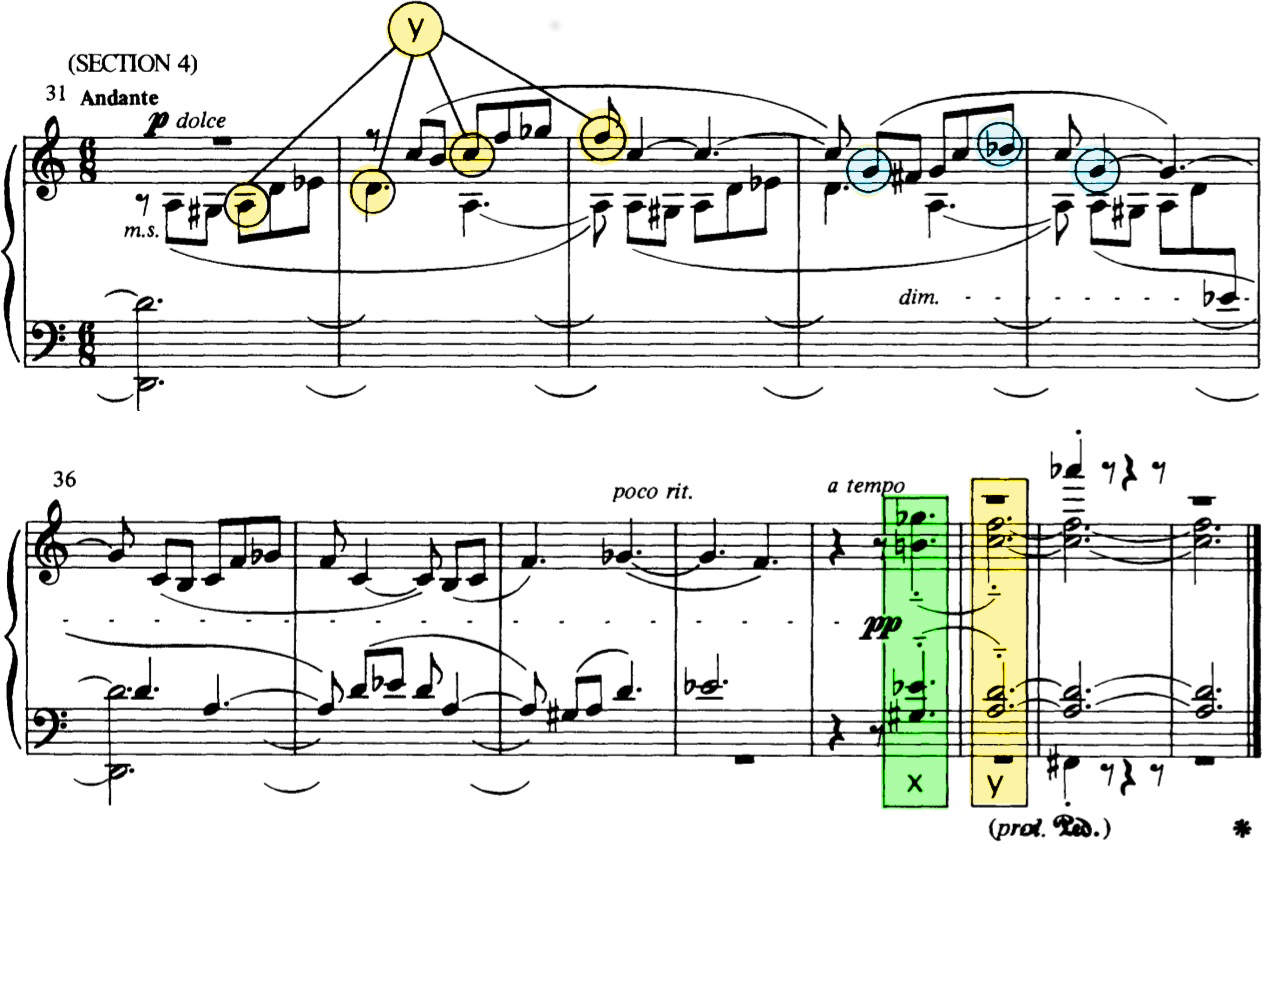
\includegraphics[scale=0.3]{octa/mikro_Bali02.png}
	\end{center}
	\legend{Fonte: autor }
\end{figure}

Na figura 37, o patch de OpenMusic que faz a redução das permutações da octatônica formada pela justaposição de coleções 4-26 demonstra também algumas particularidades: a) é possível formar duas ordenações de octatônicas que são derivadas destas tétrades b) estas quatro tétrades formam segmentos iniciados pelas notas dos extremos do sistema da eixos apontado por Lendvai\footnote{Rever \autoref{lendvai_eixos}. } [Dó, Mi$\flat$, Sol$\flat$, Lá]; c) São considerados \textit{"combinações transpositivas"}\ apenas os intervalos de 3 e 5 semitons pois encontram pares dentro da própria tétrade. É no entanto interessante observar que a presença de intervalos de terça maior e tom inteiro podem auxiliar na estratégia de uso da coleção.


\begin{figure}[!h]
	\caption{\label{fig_grafico} Coleção 4-26 }
	\begin{center}
	    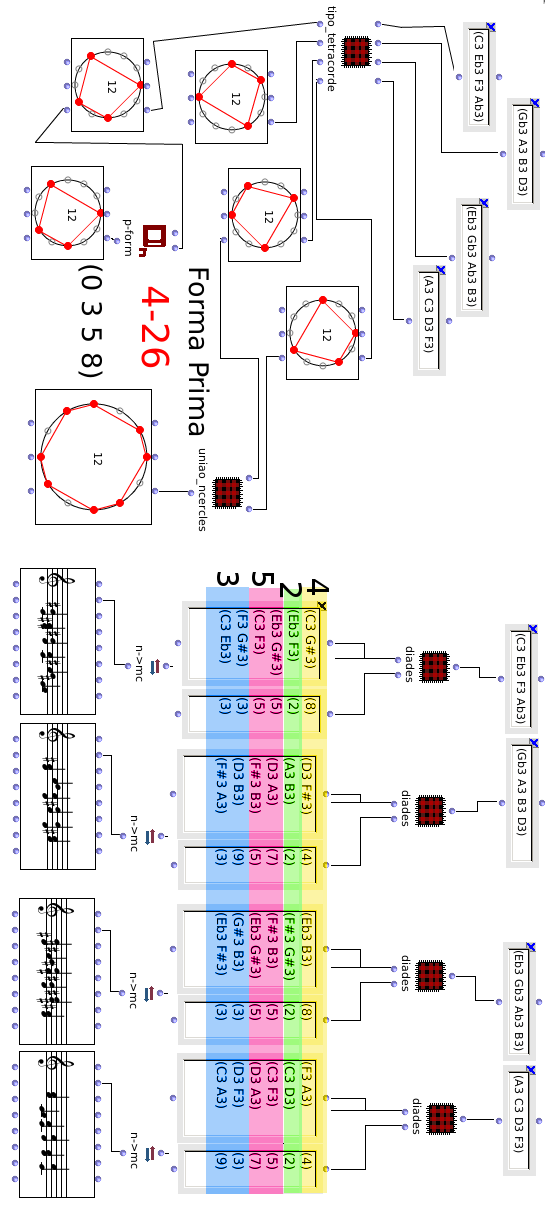
\includegraphics[scale=0.5]{octa/permuta4_26.png}
	\end{center}
	\legend{Fonte: autor }
\end{figure}






%\subsection{Combinação transpositiva em Mikrokosmos 109}

%resumo e comentários sobre \cite[ 272-275]{cohn1991bartok}

\section{Modalismo e estratégias rotacionais}
\label{modalismo}

A construção de estratégias composicionais que destacam identidades de escalas modais é traço fundamental para entendimento de repertórios que buscavam hibridizar melodias populares com arranjos e harmonizações da música artística ocidental nas primeiras décadas do século XX. 

Apesar da música de Bartók ser frequentemente associada a um apelo folclorista, devido a suas pesquisas na música camponesa do leste europeu que sempre influenciaram seu trabalho, é importante destacar que ele sempre o aproximou as melodias a de uma linguagem moderna e proto-serialista - ainda mais depois de exilado nos Estados Unidos e obviamente tocado pela catástrofe que derivou dos nacionalismos que racharam a Europa nas duas guerras mundiais que presenciou.

Danielle \citeonline{fosler2007music} aponta ainda de maneira interessante em seu livro \textit{"Music divided: Bartók's legacy in cold war culture"}\ algumas evidências de que Bartók influenciou tanto músicos de vanguarda do serialismo quanto revisionistas da música artística inspirada em motivos populares. Fatores como a morte logo após a segunda guerra mundial (1945) e a singularidade de representar a figura de um exilado que trabalhou no limite entre a linguagem de pesquisa da tradição de sua terra natal e invenção contemporânea universal, contribuíram para esta ambiguidade.

É essencial portanto, apontar aqui algumas maneiras pelas quais motivos de característica mais folclórica foram usados em sua linguagem de maneira a criarem texturas que assimilam transformações pós-tonais, criando sonoridades polimodais, cromáticas e de um serialismo de forte apelo motívico.

\subsection{Modos Gregos}

Os modos \textit{gregos} ou modos \textit{eclesiásticos} são bastante conhecidos na teoria musical ocidental por já haverem servido de matriz para música litúrgica do período pré-clássico na Europa e de certa maneira sempre presentes desde a concepção da escala temperada como uma configuração de sete notas contendo dois intervalos de semitom e cinco intervalos de tom inteiro, o conceito de diatonismo. 

A escala jônia e sua sequência de [2,2,1,2,2,1] semitons estão na gênese do que hoje entendemos como "escala maior". As rotações desta configuração de intervalos, deslocando o intervalo de semitom, são as operações que determinam os demais modos. 

Quando normalizados em Dó podemos entender, ao comparar sustenidos e bemóis, que cada um dos modos pode funcionar como uma escala maior ou menor com alguns graus modificados: \textit{Jônio} - escala maior natural; \textit{Dórico} -   escala menor com sétima menor, \textit{Frígio} - escala menor com segunda menor e sétima menor; \textit{Lídio} - escala maior com quarta aumentada; \textit{Mixolídio} - escala maior com sétima menor; \textit{Eólio} - escala menor natural; \textit{Lócrio} - escala menor com segunda menor, sétima menor e quinta diminuta.

\begin{figure}[!h]
	\caption{\label{fig_grafico}Rotações dos intervalos da pentatônica, normalizados em Dó. }
	\begin{center}
	    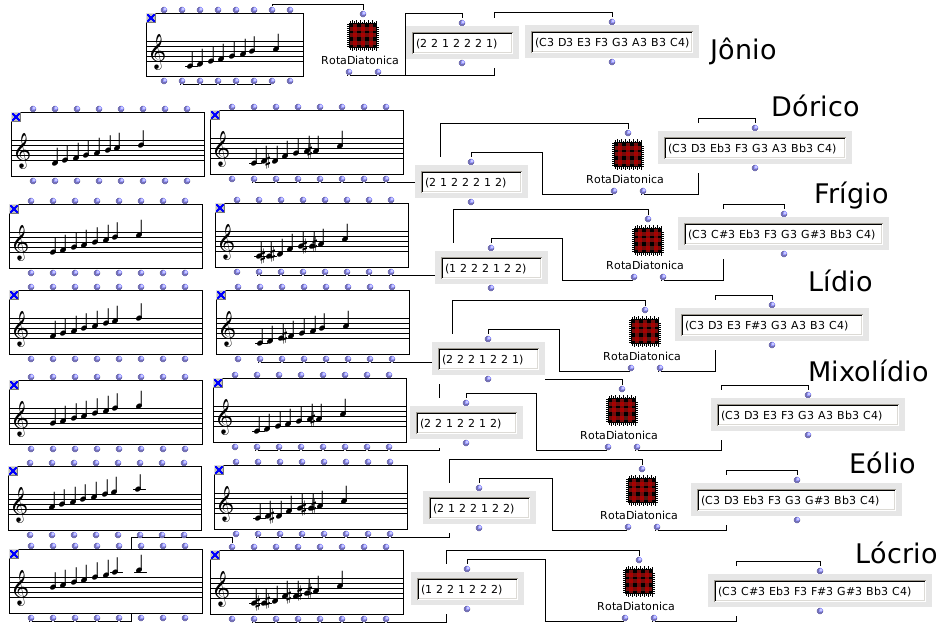
\includegraphics[scale=0.5]{modal/modal.png}
	\end{center}
	\legend{Fonte: autor }
\end{figure}


Na música de Bartók os modos gregos são utilizados também como uma estratégia de confecção de modos híbridos, introdução de coleções não-diatônicas (algumas delas resgatadas do folclore do leste europeu) e cromatismos em geral.

Uma das características recorrentes pra confecção dos modos híbridos na música de Bartok é o uso de rotações da escala pentatônica, como veremos a seguir.


\subsection{Rotação Pentatônica}
\label{pentarota}
 
\citeonline{susanni_antokoletz2012music} demonstram de maneira bastante didática algumas técnicas de rotação intervalar, transposição, união e mistura de coleções modais por inserção de notas pivô e a transformação orgânica de motivos modais ou pentatônicos em novas sonoridades híbridas não-diatônicas, cíclicas e de uma ambiguidade maior-menor, presente nesta linguagem. 

Da mesma maneira que tradicionalmente pensamos a rotação da coleção diatônica nas notas brancas do piano para memorizarmos os modos gregos\footnote{Como por exemplo: chamar as melodias iniciadas em Ré de "Modo Dórico" e delas poder reduzir uma série intervalar fixa de \textit{"0,2,3,5,7,9,10,12..."} que pode ser transposta.}, podemos também aplicar a ideia de rotação nas notas pretas do piano e considerar algumas propriedades das sequências de intervalos gerados para a sequência intervalar \textit{"0,2,5,7,9,12..."}.

\citeonline[p. 83]{susanni_antokoletz2012music} trabalham esta ideia comum ao repertório pós-tonal: de fazer a rotação da pentatônica criando uma estratégia para gerar ambiguidade em relação aos modos gregos - já que as pentatônicas não possuem os semitons que as caracterizam. Podemos então jogar com as notas faltantes como pivôs de uma transformação entre diferentes modos ou pivôs de uma simultaneidade que Bartók chamou "polimodalismo cromático" e da qual falaremos mais adiante. 

Se considerarmos a normalização da sequência tradicional das notas pretas como a transposição para os intervalos a partir de Dó ($Dó \rightarrow  Ré \rightarrow Fá \rightarrow Sol \rightarrow Lá \rightarrow Dó $) , teremos a sequência de intervalos de semitom ($Dó \rightarrow 2 \rightarrow  3 \rightarrow 2 \rightarrow 2  \rightarrow 3 \rightarrow Dó $). Iniciando \textbf{a partir de Ré} (chamemos aqui de \textbf{"rotação 2"}) teremos a rotação e intervalos ($Ré \rightarrow Fá \rightarrow Sol \rightarrow Lá \rightarrow Dó \rightarrow Ré $) equivalentes a ($  Ré \rightarrow 3 \rightarrow  2 \rightarrow 2 \rightarrow 3  \rightarrow 2 \rightarrow Ré $) e assim por diante.\footnote{Interessante notar aqui que a pentatônica a partir de Sol gera uma sequência de intervalos que pode ser particionada simetricamente. Veremos na Sessão mais adiante estratégias de uso das simetrias.}

Pensemos também que a partir desta configuração de intervalos podemos normalizar todas as sequências em uma mesma nota raiz de transposição. Por exemplo, a sequência intervalar \textbf{"a partir de Ré"}, demonstrada no parágrafo anterior como a \textbf{"rotação 2"},\ se transposta para ter \textbf{a nota Dó como raiz}, ficaria com a configuração: $Dó \rightarrow Mi\flat \rightarrow Fá \rightarrow Sol \rightarrow Si\flat \rightarrow C $ .

É a partir disso que \citeonline[p. 84]{susanni_antokoletz2012music} demonstram que estas rotações da pentatônica e suas transposições servem como uma maneira de construir transformações entre diferentes modos usando como pivô uma ou mais rotações ou transposições de um motivo pentatônico. 


Por exemplo, uma estratégia de ambiguidade entre modo Lídio e Mixolídio:

Pentatônica: $ C - D \rightarrow [ ?? ] - E - G - A \rightarrow [ ?? ] - (...) $ 

Lídio: $ C - D \rightarrow [ F\sharp ] - E - G - A \rightarrow [ B ] - (...) $  

Mixolídio: $ C - D \rightarrow [ F ] - E - G - A \rightarrow [ B\flat ] - (...) $  


A inserção de jogos de tensão com a célula [ B - F$\sharp$ - F - B$\flat$ ] mostra-se portanto uma estratégia possível para as transições deste polimodo.

\begin{figure}[!h]
	\caption{\label{fig_grafico}Rotações dos intervalos da pentatônica, normalizados em Dó. }
	\begin{center}
	    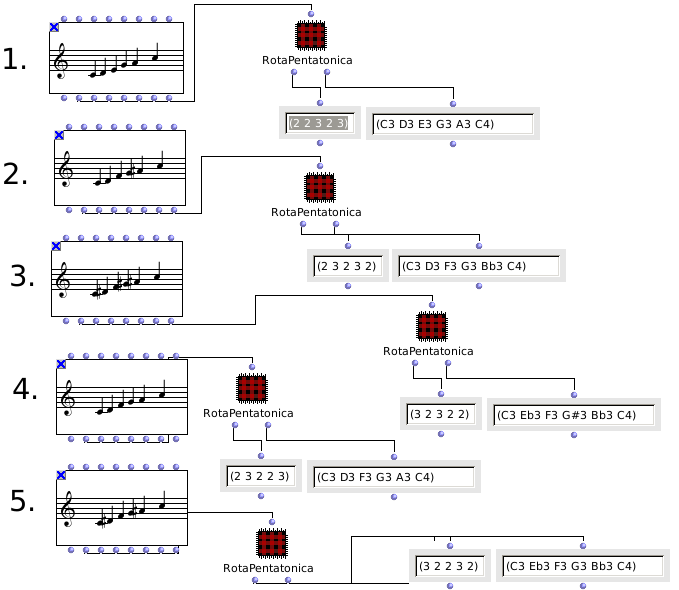
\includegraphics[scale=0.6]{OM_settheory/pentarotacoes.png}
	\end{center}
	\legend{Fonte: autor }
\end{figure}

\subsection{Cromatismo Polimodal}
\label{polimodal}

Algumas das construções de polimodos servem também como uma maneira de amenizar a entrada de cromatismos - em algumas situações introduzindo todas as 12 notas da escala cromática de maneira sutil. 

Diferente da intenção dodecafônica que buscava construir uma escuta de equilíbrio e equivalência entre os doze intervalos, Bartók trabalha aquilo que chama de "cromatismo polimodal",\ construindo estratégias de polarização - sem no entanto usar o cromatismo como uma estratégia de função tonal pura e simples. Em suas palavras:

\begin{citacao}
Como resultado de sobrepor os pentacordes Lídio e Frígio com um tom comum fundamental, nós conseguimos um pentacorde diatônico preenchido com todos possíveis sustenidos e bemóis. Estes graus aparentemente cromáticos, contudo, são totalmente diferentes de duas funções de graus alterados nos estilos cromáticos dos períodos prévios. Uma nota com alteração cromática em um acorde esta em relação estrita com sua forma não-alterada; é a transição conduzindo ao respectivo tom do acorde de resolução. Em nosso cromatismo polimodal, no entanto, os tons bemóis e sustenidos não são totalmente graus alterados; eles são ingredientes diatônicos de uma escala diatônica modal. \cite[p. 367]{bartok1993bela}\footnote{As the result of superposing a Lydian and Phrygian pentachord with a common fundamental tone, we get a diatonic pentachord filled out with all the possibe flat and sharp degrees. These seemingly chromatic degrees, however, are tottaly different in their function from the altered degrees of the chromatic styles of the previous periods. A chromatically altered note of a chord is in strict relation to its non-altered form; it is a transition leading to the respective tone of following chord. I our polymodal chromaticism, however, the flat and the sharp tones are not altered degrees at all; they are diatonic ingredients of a diatonic modal scale.\cite[p. 367]{bartok1993bela}}
\end{citacao}


\begin{figure}[!h]
	\caption{\label{fig_grafico}Rotações dos intervalos da pentatônica, normalizados em Dó. }
	\begin{center}
	    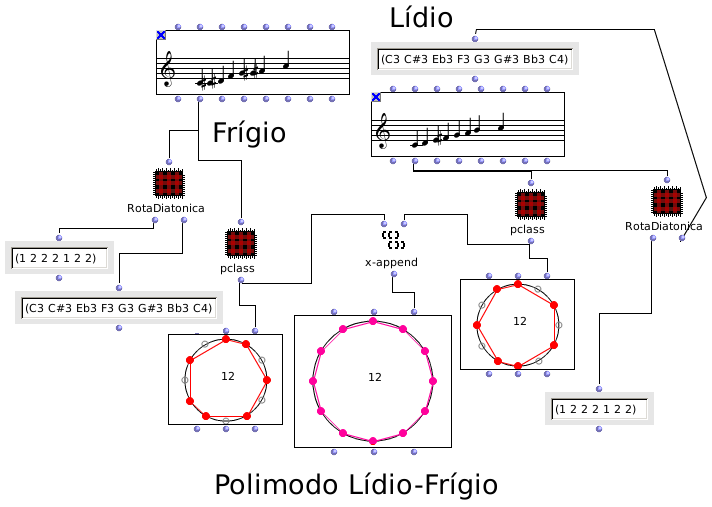
\includegraphics[scale=0.5]{modal/lidiofrigioOM.png}
	\end{center}
	\legend{Fonte: autor }
\end{figure}


\section{Harmonização dos Modos Folclóricos}


A harmonização  bartokiana em muitos casos é desamarrada das cadências tonais pela intenção de destacar a sensação modal ou pentatônica das melodias. Esta foi também uma estratégia para criar harmonizações onde as tríades maior e menor são usadas de modo ambíguo, simultâneo e que facilitam o uso do total cromático. 

Também ao evitar a sensível, surge a preferência no uso de intervalo de sétima menor como uma sonoridade sem expectativa de resolução de tonalidade que torna este intervalo na música de Bartók um traço \textit{"tão importante quanto as observação das terças e quintas na harmonia funcional tonal"} \cite[p. 28]{antokoletz1984music}. 

A simetria interna do acorde de sétima menor - (0,3,7,10) semitons empilhados formando uma estrutura de intervalos de (3-4-3) semitons - contribui para uma sonoridade ambígua, característica do polimodalismo. Função similar com sonoridade distinta também pode ser conseguida com o uso de tríades maiores de quinta aumentada e/ou tétrades menores com quinta diminuta e sexta maior, que como já vimos na \autoref{ciclos}, geram um empilhamento simétrico de intervalos.

Nas palavras do próprio Bartok, sobre a estratégia de usar acordes com empilhamentos não convencionais das terças:

\begin{citacao}
"Quanto mais simples a melodia mais complexa e estranha pode ser a harmonização e acompanhamento que vai bem com esta(...) Estas melodias primitivas, de alguma maneira, não mostram traço de junção estereotipada das tríades(...) Isto nos permite trazer a melodia mais claramente ao construir harmonias de espectro mais amplo variando ao longo de diferentes polarizações"
 \cite[p. 342]{bartok1993bela}\footnote{The simpler the melody the more complex and stranger maybe the harmonizationban accompaniment that go well with it(...)These primitive melodies, moreover, show no trace of the stereotyped joining of triads(...)It allows us to bring out the melody more clearly by building round it harmonies of the widest range varying along different keynotes. \cite[p. 342]{bartok1993bela}}
\end{citacao}


É importante também destacar que muitas vezes Bartók utiliza uma linha pentatônica no baixo, que serve para atenuar o cromatismo enquanto introduz estrategicamente com a melodia\footnote{E vice-versa com a pentatônica na melodia e cromatismos no baixo.} notas estranhas a pentatônica criando texturas polimodais, octatônicas ou na maneira mais geral algo que ele próprio chamava de "Cromatismo polimodal"\cite{antokoletz1984music}


\begin{citacao}
Para as características gerais, exatamente o mesmo pode ser dito sobre minhas melodias como eu já disse a respeito das melodias folclóricas cromáticas. Isto é, os tons destas melodias são tons independentes que não tem nenhuma interrelação entre si. Há em cada espécie, no entanto, uma fundamental decididamente fixa na qual outros tons resolvem no fim. A diferença principal entre as melodias folclóricas cromáticas e as minhas próprias melodias cromáticas podem ser encontradas no seu registro. As melodias folclóricas consistem exclusivamente de cinco, seis ou no máximo sete semitons, que correspondem a um alcance em torno da quarta justa. Minhas melodias tem geralmente pelo menos oito semitons e combrem, em alguns casos, a distância de uma oitava ou mais.\cite[p. 381]{bartok1993bela}\footnote{
As to the general characteristics, exactly the same can be said about my melodies as what I said already concerning the chromatic folk melodies. That is, the single tones of these melodies are independent tones having no interrelation between each other. There is in each specimen, however, a decidedly fixed fundamental tone to which the other tones resolve in the end. The main difference between the chromatic folk melodies and my own chromatic melodies is to be found in their range. They consist exclusively of five, six, or at most seven half-tones, which corresponds to a range of about a fourth. My own melodies generally have at least eight half-tones and cover, in some cases, the distance of an octave or more.\cite[p. 381]{bartok1993bela}}
\end{citacao}

\pagebreak
Um exemplo interessante desta estratégia de separar as coleções entre um ostinato ou cadência de acordes na mão direita e uma melodia com uma coleção de intervalos distinto na mão esquerda é o Mikrokosmos nº 125, \textit{"Boating"}. Nesta peça podemos ver claramente na partitura a separação das linhas do baixo e melodia - pois a mão direita está fazendo ostinatos em saltos de quarta nas \textit{"notas brancas"} do piano, enquanto a mão esquerda está fazendo a melodia pentatônica nas \textit{"notas pretas"}. 

\begin{figure}[!h]
	\caption{\label{fig_grafico}Ostinatos nas notas brancas e melodia nas notas pretas em Mikrokosmos 125 }
	\begin{center}
	    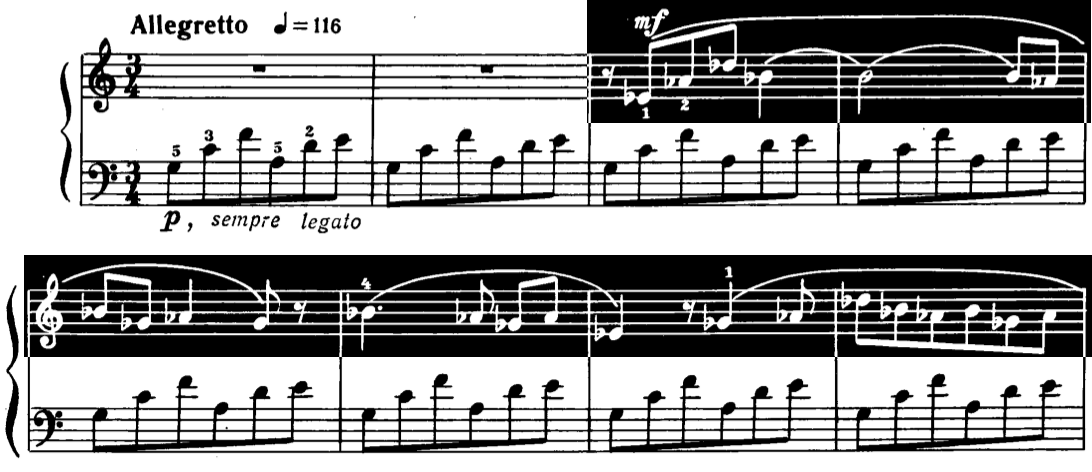
\includegraphics[scale=0.45]{ostinatos/boating_ostinato.png}
	\end{center}
	\legend{Fonte: autor }
\end{figure}

Na \autoref{m21} fazemos uma análise assistida por computador de Mikrokosmos 41, onde demonstramos uma estatégia de construção polimodal e simultânea a uma melodia de sonoridade pentatônica.



%\subsection{Limites e ideias a partir de analise tonal funcional}
%\label{Prolongamento}

%comparação com algoritmo de key probing
%\cite{cooper1998unfolding}


%usar analise e comentario sobre mikro 100 e 101 do paper 25bartokshenker limits
%\cite[p. 179]{brown1997iv}

%comentario de  mikro101 em strauss
%\cite[p. 113]{straus2004}

%
%
%
%%%%%%%%%%%%%%%%%%%%%%%%%%%%%%%%%%%%%%%%%

\part{Formalizações Computacionais}


\chapter{Análise Musical Assistida por Computador}
\label{analise_computacional}

Este capítulo elabora sobre as possibilidades de uma análise musical assistida por computador através de um estudo comparado entre duas ferramentas livres:\footnote{Consideramos aqui o conceito de "software livre" a partir da definição das 4 liberdades, propostas por Richard Stalmann:\textit{ A liberdade de executar o programa como você desejar, para qualquer propósito (liberdade 0). A liberdade de estudar como o programa funciona, e adaptá-lo às suas necessidades (liberdade 1). Para tanto, acesso ao código-fonte é um pré-requisito. A liberdade de redistribuir cópias de modo que você possa ajudar ao próximo (liberdade 2). A liberdade de distribuir cópias de suas versões modificadas a outros (liberdade 3). Desta forma, você pode dar a toda comunidade a chance de beneficiar de suas mudanças. Para tanto, acesso ao código-fonte é um pré-requisito.}} a biblioteca Python Music21 e a linguagem dataflow\footnote{Entendemos aqui como dataflow as linguagens onde temos fluxogramas gráficos que podem ser manipulados funcionalmente, permitindo que \textbf{o projeto do algoritmo de um código seja já seu próprio código.}} OpenMusic.

Parte das aplicações práticas já foram demonstradas nos exemplos dos capítulo anterior, mas aqui explico em mais detalhes os conceitos e procedimentos computacionais utilizados.


\section{Formatos de entrada}


Os formatos de arquivos utilizados nas análises estão dentro do paradigma de representação simbólica de conteúdos musicais, isto é: são organizados como um mapa temporal de parâmetros gestuais sobre determinada nota (ou conjuntos de notas) a ser ouvida sob determinado timbre (em todos casos aqui, um piano) não incluso como parte do arquivo. 

Arquivos sonoros de performances instrumentais das composições ou as renderizações de timbres de arquivos simbólicos não estão sendo levados em conta na pesquisa por estarem fora do escopo no momento.



\subsection{MIDI}

Por muito tempo o formato MIDI ficou estigmatizado por ser associado aos timbres genéricos da indústria de sintetizadores populares dos anos 80 e 90 e pelas primeiras placas de som e softwares sequênciadores de eventos ou partituras dos computadores pessoais. 

Na verdade o formato não carrega parâmetros de timbres em seus metadados. Um arquivo MIDI carrega valores básicos de expressão sobre a força e a duração da nota e as alturas cromáticas que devem ser moduladas, permitindo que esta seja posteriormente associada a qualquer timbre.

É importante ter em mente que o protocolo MIDI, por ser há mais de 35 anos um padrão ainda em uso, gerou um legado relevante de arquivos baseados em repertório clássico para a reconstituição de \textit{corpus} de peças partituradas. 

Porém, apenas estes parâmetros oferecidos por padrão pelo protocolo MIDI não são descritores capazes de garantir a boa formatação de seus dados como figuras de compasso de uma pauta tradicional, já que os arquivos MIDI não carregam informações sobre as figuras, apenas sobre as durações, alturas e expressão das notas.

Quando importados para programas de notação ou convertidos para formatos destes, os arquivos MIDI irão passar por uma segmentação arbitrária e determinada pelo algoritmo \textit{"parser}"\footnote{Método computacional para conversão entre formatos ou tipos de dados diferentes.}, que vai converter determinada duração em determinada métrica quantizada, normalmente diferente das articulações a partir das quais as músicas foram digitalizadas.


\subsection{Lilypond}

Lilypond é uma  \textit{"linguagem de marcação"}\ similar à linguagem Latex (para formatação de documentos científicos), que também possui um compilador próprio, pode gerar partituras em formato final de imagem, pdf ou arquivos MIDI para renderização sonora.

O objetivo principal no Lilypond é a formatação de uma notação partitural avançada e otimizada para impressão em papel. Permite também a utilização de elementos de notação mais exótica, como inclusão de texto, dedilhados, nomenclatura de acordes, sinais de expressão, e customização de elementos a partir de módulos. Facilita a otimização da disposição e dimensão das fontes dos objetos e possui uma linguagem \textit{script} própria, dialeto da sintaxe \textit{scheme}\footnote{Tutorial oficial de lilypond-scheme: \url{http://lilypond.org/doc/v2.16/Documentation/source/Documentation/extending/introduction-to-scheme} Acesso em 10 de julho de 2014.}.

No presente trabalho, estamos utilizando Lilypond como um arquivo de saída ou um arquivo intermediário (de conversão entre arquivos), pois as ferramentas utilizadas aqui não possuem parsers satisfatórios para tratar uma \textbf{entrada} em Lilypond, apesar de serem capazes de gerar saída no formato .ly.


\begin{figure}[htb]
	\caption{\label{fig_grafico}Gerador de um acorde Dó maior (dó4 e4 g5) na clave de sol em Lilypond}
	\begin{center}
	    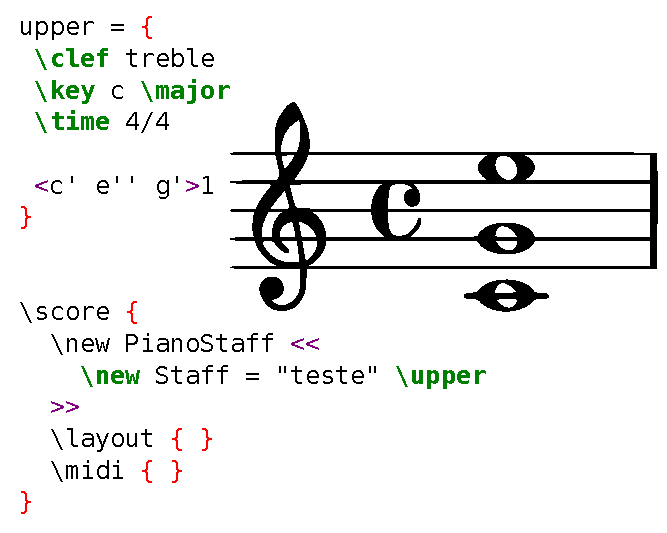
\includegraphics[scale=0.75]{score/lilypond.pdf}
	\end{center}
	%\legend{Fonte: autor}
\end{figure}


\subsection{MusicXML}

O uso geral do formato MusicXML é similar ao Lilypond - formatação de partituras. No entanto, enquanto Lilypond é um sistema completo fechado em si próprio, o MusicXML é um formato com a potência de se tornar um padrão intercambiável entre diferentes aplicações de partitura\footnote{ Lista atualizada de aplicações compatíveis com o formato MusicXML: \url{http://www.musicxml.com/software/} Acesso em 10 de julho de 2014.}.


\begin{figure}[htb]
	\caption{\label{fig_grafico}Gerador de uma nota dó4 na clave de sol em MusicXML}
	\begin{center}
	    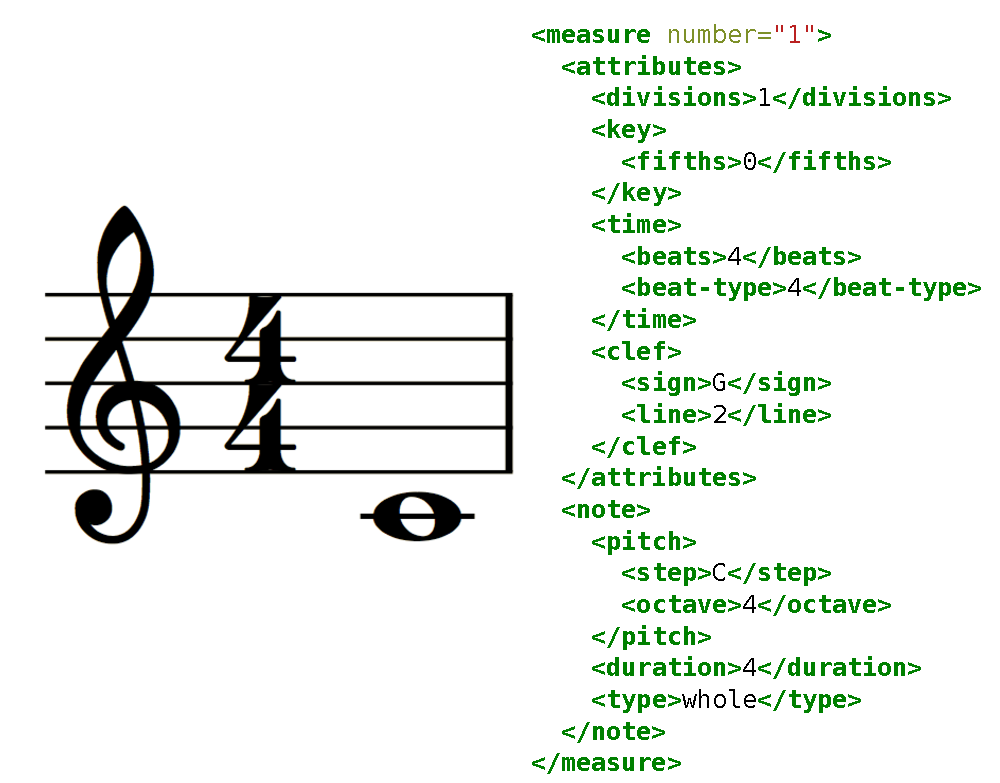
\includegraphics[scale=0.5]{score/musicxml.pdf}
	\end{center}
	%\legend{Fonte: autor}
\end{figure}


\section{Music21}
\label{m21}

É uma biblioteca projetada para trabalhar com manipulação e análise de \textit{corpus} de arquivos partituráveis\footnote{\url{http://goo.gl/ovMEl1} Acesso em 10 de julho de 2014.}. Prepara a conversão entre diversos arquivos de dados musicais (MIDIs, humdrum, lilypond, abc)\footnote{\url{http://goo.gl/K9GQ01} Acesso em 10 de julho de 2014.}, mas nativamente trabalha com uma estrutura de dados baseada em Music XML.

Music21 tem uma abordagem voltada para uma "musicologia assistida por computador"\ e já tem incorporada em suas classes algumas ferramentas comuns a esta prática como: numeração de grau funcional de acorde\footnote{\url{http://goo.gl/n1DgAN} Acesso em 10 de julho de 2014.}, numeração de classes de altura usando a classificação de Allen Forte\footnote{\url{http://goo.gl/Pkbcig}Acesso em 13 de fevereiro de 2015.}: a implementação dos algoritmos de detecção de tonalidade\footnote{\url{http://goo.gl/vj8LyB} Acesso em 10 de julho de 2014.} elaborado por \citeonline{krumhansl1990cognitive} e aperfeiçoada por \citeonline{temperley2001cognition}, busca de padrões como transposições e inversões\footnote{\url{http://goo.gl/BrrLer}Acesso em 13 de fevereiro de 2015.} e outros.\footnote{{\url{http://goo.gl/ejiCMP}Acesso em 13 de fevereiro de 2015.}}



\subsection{Stream}

A biblioteca Music21 tem como uma das ideias básicas a estrutura de dados "Stream"(Fluxo). Esta estrutura de dados funciona como uma subclasse da classe music21, estruturas as quais a documentação\footnote{\url{http://goo.gl/lNMMLJ}Acesso em 13 de fevereiro de 2015.} refere-se  como "módulos". Um Stream irá conter dentro dele uma estrutura de dados semelhante a uma lista Python, ordenando em sequência os instrumentos, claves, assinaturas de compasso, notas, acordes, pausas, ornamentos.

Para entender a estrutura de dados na prática, vejamos os procedimentos a seguir. Demonstramos em um script Python\footnote{Para uma introdução básica ao Python a partir de uma perspectiva musical conferir \cite{Kroger201208} }, comentado linha a linha\footnote{Todos os comentários dos códigos Python mostrados aqui estão próprio no corpo do código em linhas que possuem o sinal de sustenido ( \# ) no início.}, um procedimento mínimo para inserir um acorde dentro de um fluxo e renderizá-lo em uma partitura em pdf.

 
\begin{lstlisting}
#Importando a biblioteca
from music21 import *

#Criando um objeto de fluxo 
fluxo = stream.Stream()

#Criando um objeto acorde
acorde=chord.Chord(['C4','A4','E5'])

#Adicionando o objeto acorde no inicio do fluxo
fluxo.insert(0,acorde)

#Renderizando em pdf
fluxo.show('lily.pdf')
\end{lstlisting}
 

\begin{figure}[!h]
	\caption{\label{fig_grafico} A saída do teste em terminal cria um arquivo temporário em pdf com a renderização do Stream.}
	\begin{center}
	    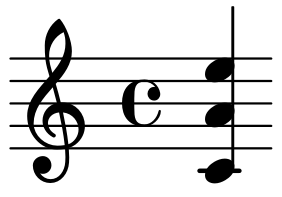
\includegraphics[scale=0.3]{estudosM21/acorde01.png}
	\end{center}
	\legend{Fonte: autor }
\end{figure}

O script insere um objeto acorde na posição zero do fluxo. Podemos perceber pela figura acima que por padrão a biblioteca renderizou a pauta em uma clave de Sol com assinatura de compasso quatro por quatro. Em uma situação mais complexa obviamente temos muito mais pra pensar: teremos instrumentos de duas pautas como piano, ornamentos, texto, pautas com fórmulas de compasso diferentes, e assim por diante.

Precisaremos separar as partes hierarquicamente, criando uma estrutura de dados em camadas, como vemos no exemplo mais complexo abaixo. 


\begin{lstlisting}

# Criamos um objeto score (partitura) para usar como fluxo
partitura=stream.Score()

# Separamos o fluxo em duas partes: duas pautas
mao_esquerda=stream.PartStaff()
mao_direita=stream.PartStaff()

# Criamos os compassos para cada pauta 
compasso1L=stream.Measure(number=1)
compasso1R=stream.Measure(number=1)

# Necessitamos formatar o layout do score para agrupar as duas pautas
compasso1L.insert(0,layout.SystemLayout())
compasso1L.insert(0,layout.StaffLayout(staffNumber=2))

# Inserindo a clave, a formula de compasso, nota e acorde
compasso1L.insert(0,clef.BassClef())
compasso1L.insert(0,meter.TimeSignature('2/4'))
compasso1L.insert(0,note.Note('F3'))
compasso1L.insert(1,chord.Chord(['A2','E3','C4']))

# Inserindo o compasso da pauta da mao esquerda na parte inferior
mao_esquerda.insert(0,compasso1L)

# Inserindo a clave, a formula de compasso, nota e pausa
compasso1R.insert(0,layout.SystemLayout())
compasso1R.insert(0,clef.TrebleClef())
compasso1R.insert(0,meter.TimeSignature('2/4'))
compasso1R.insert(0,note.Note('C5'))
compasso1R.insert(1,note.Rest())

# Inserindo o compasso da pauta da mao direita na parte superior
mao_direita.insert(0,compasso1R)

# Formatando a entrada das partes na camada de layout da partitura
partitura.insert(0,mao_direita)
partitura.insert(0,mao_esquerda)

# Renderizando em PDF
partitura.show('lily.pdf')
\end{lstlisting}

\begin{figure}[!h]
	\caption{\label{fig_grafico} Renderização da pauta de piano em compasso $2/4$} 
	\begin{center}
	    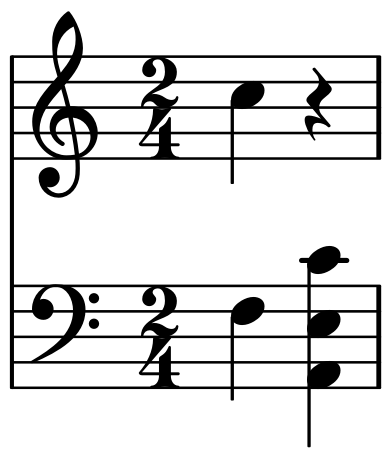
\includegraphics[scale=0.25]{estudosM21/pautaM21.png}
	\end{center}
	\legend{Fonte: autor }
\end{figure}

Importante também destacar aqui que a proposta maior da biblioteca Music21 é a de servir como auxiliar em processos de análise de partituras. 

Temos portanto uma série de procedimentos que permitem que partituras formatadas exteriormente (em formatos como musicxml, abc, humdrum, midi, etc.) sejam carregadas e convertidas para a estrutura de dados da biblioteca, facilitando sua análise, manipulação e re-modelagem. 

O script anterior obviamente pode ser encapsulado em uma função, utilizando recursividade e algumas outras funções presentes na biblioteca para evitar tanto código para cada compasso. 

No entanto, dessa maneira passo a passo fica entendido que a formatação das partituras ocorre de maneira similar ao padrão xml de encapsulamento de dados: temos camadas dentro de camadas que vão da página de impressão até os acordes, notas, pausas e ornamentos.

Vejamos abaixo como é feita a conversão de uma partitura com o mesmo conteúdo gerado anteriormente, mas desta vez criada em um editor de partituras e salva no formato musicxml\footnote{Editada no software livre Musescore.}. No script abaixo nós abrimos o arquivo dentro de um terminal Python e em seguida imprimimos para mostrar como ela fica formatada dentro da estrutura de dados do Music21.

\begin{lstlisting}
>>> p=converter.parse('piano.xml')
>>>p. show('text')

{0.0} <music21.metadata.Metadata object at 0xb3f642c>
{0.0} <music21.stream.PartStaff P1-Staff1>
    {0.0} <music21.instrument.Instrument P1: Piano: Piano>
    {0.0} <music21.stream.Measure 1 offset=0.0>
        {0.0} <music21.layout.SystemLayout>
        {0.0} <music21.clef.TrebleClef>
        {0.0} <music21.key.KeySignature of no sharps or flats, mode major>
        {0.0} <music21.meter.TimeSignature 2/4>
        {0.0} <music21.note.Note C>
        {1.0} <music21.note.Rest rest>
        {2.0} <music21.bar.Barline style=final>
{0.0} <music21.stream.PartStaff P1-Staff2>
    {0.0} <music21.instrument.Instrument P1: Piano: Piano>
    {0.0} <music21.stream.Measure 1 offset=0.0>
        {0.0} <music21.layout.SystemLayout>
        {0.0} <music21.layout.StaffLayout staffNumber 2>
        {0.0} <music21.clef.BassClef>
        {0.0} <music21.key.KeySignature of no sharps or flats, mode major>
        {0.0} <music21.meter.TimeSignature 2/4>
        {0.0} <music21.note.Note F>
        {1.0} <music21.chord.Chord A2 E3 C4>
        {2.0} <music21.bar.Barline style=final>
{0.0} <music21.layout.ScoreLayout>


\end{lstlisting}

O que vemos aqui é uma estrutura bastante similar à que geramos no script anterior. A impressão da estrutura dos dados facilita que enxerguemos a maneira aninhada com que os dados são inseridos em camadas uns dentro dos outros.

Se analisarmos a partitura que esta alocada dentro da variável "p"\ como se fosse uma lista Python comum, veremos que o que temos são listas dentro de listas, o que permite que usemos métodos comuns de iteração normalmente usados em Python.

\begin{lstlisting}
>>> p[0]
<music21.metadata.Metadata object at 0xb3f642c>
>>> p[1]
<music21.stream.PartStaff P1-Staff1>
>>> p[2]
<music21.stream.PartStaff P1-Staff2>
>>> p[2][0]
<music21.instrument.Instrument P1: Piano: Piano>
>>> p[2][1]
<music21.stream.Measure 1 offset=0.0>
>>> p[2][1][0]
<music21.layout.SystemLayout>

>>> p[2][1][5]
<music21.note.Note F>
>>> p[2][1][6]
<music21.chord.Chord A2 E3 C4>
>>> acorde=p[2][1][6]

>>> for i in acorde:
...     print i
... 
<music21.note.Note A>
<music21.note.Note E>
<music21.note.Note C>

\end{lstlisting}

  
 
\subsubsection{Notas, Acordes e nomenclaturas}

Como vemos no final do experimento acima o objeto acorde pode ser entendido no Music21 como uma lista de objetos nota. Das relações entre objetos nota é possível também extrair intervalos ou transpor notas individuais do acorde. É possível também aplicar transformações e inferências diretamente no objeto acorde.

Alguns exemplos:

\begin{lstlisting}

# Iniciamos copiando um acorde menor normalizado em Do, usando a tabela de Forte(1973)
>>> c=chord.fromForteClass('3-11')
>>> c
<music21.chord.Chord C E- G>

# Necessitamos definir a oitava, caso contrario o acorde fica sempre no registro C4
# o metodo 'closedPosition' coloca as notas em ordem crescente e mais proxima
>>> c.closedPosition(forceOctave = 3, inPlace= True)
>>> c
<music21.chord.Chord C3 E-3 G3>

# Criamos uma copia transposta do acorde, podemos utilizar nomes (abreviados)  
#de intervalos como '6M' para sexta maior
>>> a=c.transpose('6M')
>>> a
<music21.chord.Chord A3 C4 E4>

# Temos um metodo para transformar ou inferir inversoes do acorde
>>> a.inversion(1)
>>> a
<music21.chord.Chord C4 E4 A4>

>>> a.inversion(2)
>>> a
<music21.chord.Chord E4 A4 C5>

# Um acorde pode tambem ser inicizado com umas lista de notas e suas oitavas
>>> A=chord.Chord(['A4','C#4','E4'])

#Podemos inferir seu nome "comum", no caso das triades temos 
#os nomes funcionais da harmonia tradicional
>>> A.pitchedCommonName
'A4-major triad'

# E seu nome equivalente na tabela de Forte
>>> A.forteClass
'3-11B'

# Podemos transpor notas especificas do acorde
>>> a=chord.Chord([a[0],a[1].transpose(interval.Interval(-1)),a[2]])
>>> a
<music21.chord.Chord E6 G#6 C6>

# Todas as cardinalidades da tabela de Forte estao presentes
>>> o=chord.fromForteClass('8-28')
<music21.chord.Chord C C# E- E F# G A B->
# Lembrando que o bemol no Music21 e trocado de 'b' para '-' (ex: Eb fica E-) 

# A forma prima fonece o valor dos intervalos em sua ordem crescente 
#e normalizada a partir de zero
>>> o.primeForm
[0, 1, 3, 4, 6, 7, 9, 10]


\end{lstlisting}


\subsection{Cadência e inferência de tonalidade}


O Music21 fornece uma série de ferramentas para análise de harmonia funcional, incluindo algoritmos para sugerir grau cadencial (com o uso de numerais romanos) e de detecção de regras de contraponto na condução de vozes. Obviamente que, para que tudo isso tenha um sentido estritamente tonal, teríamos que estar analisando repertórios que se encaixam nos padrões da "prática comum" \cite[p. 354]{temperley2001cognition} podendo ater-se aos pequenos desvios da norma como invenção estilística dos compositores. Por outro lado, o uso deste tipo de ferramenta em repertórios pós-tonais pode tomar um sentido interessante. 

Em seu artigo \textit{"The unfolding of tonality in the music of Béla Bartók"},\ David \citeonline{cooper1998unfolding} propõe a análise assistida por computador das \textit{"10 Easy Piano Pieces"} de Bartók. 

Após testar os mesmos algoritmos de detecção de tonalidade que usou para analisar as peças do \textit{"Cravo Bem Temperado"} de J. S. Bach, onde obteve uma aproximação muito satisfatória das análises conhecidas da obra, Cooper conclui que o mesmo procedimento também ajudaria o analista a inferir ideias sobre ambiguidade ou politonalidade em compositores pós-tonais como Bartók,  mesmo com alguns desvios previstos.

Por ser independente de estilo, o algoritmo poderia ajudar a revelar estruturas implícitas e residuais do condicionamento tonal da escuta, isto é, sua força estaria justamente em revelar, mesmo através de "erros"\ formais da funcionalidade estilística, dados que podem gerar ideias para o analista.

\begin{citacao}
Apesar de em essência o algoritmo ser fundamentalmente ignorante musicalmente, 'sabendo' pouco sobre estrutura musical e nada de estética, este é capaz de simular de maneira bem sucedida uma habilidade musical específica, que é determinar tonalidade global e local. Contudo, é por causa da ausência de critério artístico que este pode ser uma ferramenta útil para o repertório do analista, providenciando uma medida de tonalidade que seja amplamente independente de conhecimento "dependente de estilo'.\cite[p. 34-35]{cooper1998unfolding}.\footnote{Although in itself the algorithm is fundamentally musically ignorant, 'knowing' little about musical structure and nothing of aesthetics, it is able to simulate quite successfully one particular musical skill, that of determining local and global tonality. Indeed, it is because of its artlessness that it could form a useful tool in the analyst's repertoire, by providing a measure of tonality which is largely independent of 'style dependent' knowledge. \cite[p. 34-35]{cooper1998unfolding}}
\end{citacao}



\subsubsection{Key Profiles} 

A redução quantitativa para construção de algoritmos para inferência de "estruturas básicas da cognição musical" \cite{temperley2001cognition}\ é uma área de pesquisa interdisciplinar entre os estudos sobre a aquisição psicossocial do repertório musical que normatiza a escuta ocidental e a formalização computacional de "gramáticas gerativas" \cite[p. 83]{nierhaus2009algorithmic},\ está muito influenciada pela formalização das disciplinas que deram origem à linguística computacional.\cite{roads1979grammars}    

A observação de parâmetros para uma inferência de cadência e prolongamento da expectativa tonal implica discussões sobre a aplicabilidade de teorias ambiciosamente "gerais"\ sobre estruturas fundamentais da escuta.


Por outro lado, uma proposta mais experimental como a de \citeonline{cooper1998unfolding} e a disponibilidade de alguns algoritmos derivados destas reflexões na biblioteca Music21 nos permitem especular a partir de algumas experiências práticas que veremos a seguir.


\begin{lstlisting}
# abrir no music21 a partitura de Mikrokosmos 41 editada em musicxml
>>> m=converter.parse('mikro041.xml')

# o metodo key do modulo analyze usa por padrao
# o algoritmo de Krumhansl(1983)
>>> ak = m.analyze('key')
>>> ak
<music21.key.Key of G major>

# o indice de zero a um de precisao para o criterio do algoritmo
>>> ak.correlationCoefficient
0.7569137256478474
#
#
# podemos buscar interpretacoes alternativas
>>> alt=ak.alternateInterpretations
>>> for i in alt:
...     i.name+" = "+str(i.correlationCoefficient)
... 
'B minor = 0.624054831613'
'A major = 0.458564195272'
'E minor = 0.455816729504'
'D major = 0.387453206313'
#(...)
# as demais alternativas apresentam coeficientes mais cada vez mais baixos 
#ate que fiquem negativos, indicando "impossibilidade" de expectativa de tonalidade
>>> 

>>> 
\end{lstlisting}

Os softwares de análise de David Temperley\footnote{http://humdrum.ccarh.org/} e David Huron\footnote{http://www.link.cs.cmu.edu/music-analysis/}  para uma segmentação computacional da expectativa tonal parecem ter colaborado para síntese de ferramentas computacionais que inspiraram alguns algoritmos da biblioteca music21, pois alguns destes podem ser encontrados nos módulos de análise.\footnote{https://github.com/cuthbertLab/music21/blob/master/music21/analysis/discrete.py}

Mas apesar de desenvolverem seus próprios algoritmos de detecção de tonalidade\footnote{\cite[p. 173]{temperley2001cognition} e \citeonline[p. 150]{huron2006sweet}}, ambos citam como referência original o algoritmo resultante da pesquisa "Krumhansl-Schmuckler"\footnote{c.f. Discussão na mailing list do Music21 sobre os algoritmos em \url{https://groups.google.com/forum/\#!topic/music21list/lwamYR0o8To}}. Este algoritmo é também utilizado como padrão na biblioteca Music21, por isso vale aqui o comentário.

O algoritmo de "Krumhansl-Schmuckler"\ surge em \textit{"Perceptual Structures of Tonal Music"}\ \cite{krumhansl1983perceptual} e é aprofundado em \textit{"Cognitive foundations of musical pitch"}\ \cite{krumhansl1990cognitive}.

Carol Krumhansl e Mark Schmukler constroem um modelo matemático que chamam "perfis-tonais"\footnote{\textit{"tonal profiles"}} - histogramas que servem como uma referência\footnote{O histograma apresenta valores para uma escala cromática normalizada no contexto de Dó maior e Dó menor. Para ser transposto para outras tonalidades, basta rotacionar a ordem das alturas.} para cálculo estatístico a partir de uma amostra de ouvintes pesquisados sobre a tendência a adaptar cognitivamente \cite[p.  173]{temperley2001cognition} notas de uma escala cromática como ornamentos dentro de um determinado contexto tonal.

A fórmula funciona da seguinte maneira\footnote{C.f. uma prova real detalhada da fórmula original em \cite[p.37]{krumhansl1990cognitive} }:

\scalebox{1.5}{%
$
r= 
\frac{\sum{(x-\overline{x})(y-\overline{y})}}
{\sqrt{ \sum{ (x-\overline{x})^2 } \sum{ (y-\overline{y})^2 } } }
$
}


$ \left\{
  \begin{array}{l l}
x = valores\;individuais\;do\;histograma\;original \\
\overline{x} = media\;de\;todos\;valores\;do\;histograma\;original \\
y = valores\;de\;um\;histograma\;a\;ser\;comparado - retirado\;de\;trecho\;musical \\
\overline{y} = media\;de\;todos\;os\;valores\;do\;histograma\;usado\;em\;y \\
    
  \end{array} \right.
$


\begin{figure}[!h]
	\caption{\label{fig_grafico}Perfis de tonalidade propostos por Carol \citeonline{krumhansl1990cognitive} - histograma demonstrado por \citeonline{temperley2001cognition}. }
	\begin{center}
	    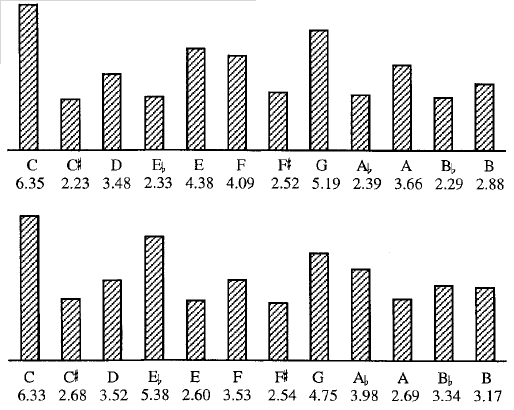
\includegraphics[scale=0.4]{CBMS/krumhansl_temperley_p174.png}
	\end{center}
	\legend{Fonte: \cite[pg. 174]{temperley2001cognition} }
\end{figure}

\begin{figure}[!h]
	\caption{\label{fig_grafico}Perfis de tonalidade propostos por Carol \citeonline{krumhansl1983perceptual} - comparativo entre tonalidades próximas e distantes. }
	\begin{center}
	    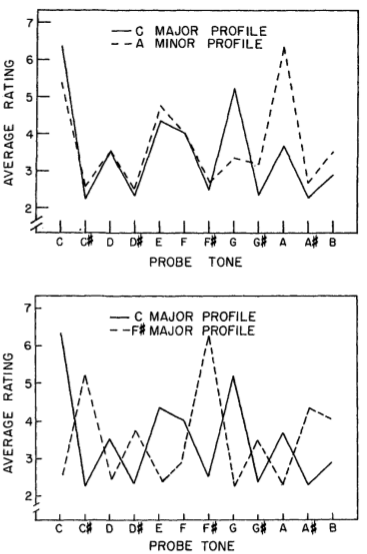
\includegraphics[scale=0.45]{CBMS/probeones_krumhansl_p36.png}
	\end{center}
	\legend{Fonte: \cite[pg. 36]{krumhansl1990cognitive} }
\end{figure}


A fórmula de perfis tonais mostra em seus resultados também uma sugestão composicional curiosa para estratégias politonais. Vemos, por exemplo, na exposição original das figuras estatísticas da comparação entre tonalidades próximas e distantes (Figura 29), as relações apontadas por Lendvai em seu sistema de eixos\footnote{ Rever \autoref{lendvai_eixos} }. 

Podemos observar que se a comparação com a tonalidade relativa menor de Dó Maior (Lá menor) possui apenas pequenos desvios, possibilitando a geração e ambiguidade, a relação com uma tonalidade de "contra-polo"\ de Dó Maior (Fá$\sharp$ Maior) tem também um efeito bastante específico: apoia-se numa expectativa simetricamente oposta de alturas, o que lembra os movimentos politonais de Bartók que buscam estabelecer estratégias de uso do total cromático por mistura de modos ou tonalidades, suspendendo as expectativas e criando vórtices para modulação.


O Music21 apresenta também um módulo para plotagem de dados bastante útil. Abaixo demonstramos a plotagem do espaço de alturas da composição Mikrokosmos 41 que revela o panaroma de uso das alturas.


\begin{lstlisting}
>>> p = graph.PlotHistogramPitchClass(m)
>>>p. process()

>>> p = graph.PlotHistogramPitchSpace(m)
>>>p. process()

>>> p = graph.PlotScatterPitchSpaceQuarterLength(m)
>>>p. process()

\end{lstlisting}


\begin{figure}[!h]
	\caption{\label{fig_grafico} Pitch Space em Mikrokosmos 41.} 
	\begin{center}
	    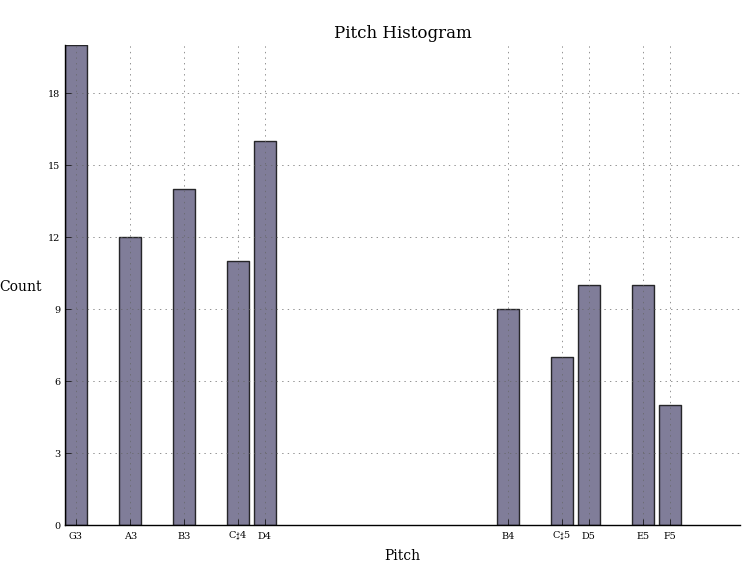
\includegraphics[scale=0.4]{estudosM21/mikro041Pspace.png}
	\end{center}
	\legend{Fonte: autor }
\end{figure}


Aplicada então a análise de tonalidade em um segmento cadencial final de Mikrokosmos 41, podemos ter um apoio estatístico para algumas conclusões:

\begin{lstlisting}
# Reduzimos as pautas do piano a uma unica pauta feita de acordes,
#facilitando a analise de graus cadenciais
>>> x=m.chordify()

# Cortamos os compassos finais
>>> X=x[11:15]
# Rodamos o algoritmo de deteccao de tonalidade
>>> K = X.analyze('key')
<music21.key.Key of G major>

# o grau de possibilidade para esta tonalidade
>>> K.correlationCoefficient
0.7319734760212024

# algumas interpretecoes alternativas - a tonalidade de Si menor
# apresenta aqui mais de 50 por cento de chance tambem
>>> alt=K.alternateInterpretations
>>> for i in alt:
...     i.name+" = "+str(i.correlationCoefficient)      
... 
'B minor = 0.583943016291'
'E minor = 0.418671671701'
'A major = 0.311484217597'

# o metodo para extrair acordes de graus cadenciais
>>> r = roman.RomanNumeral('VII', key.Key('Bm'))
>>> [str(p) for p in r.pitches]
['A5', 'C#6', 'E6']

>>> r=roman.RomanNumeral('VI', key.Key('Bm'))
>>> [str(p) for p in r.pitches]
['G5', 'B5', 'D6']

# vejamos quais os graus cadenciais possiveis para a tonalidade de sol maior
>>> R=[]
>>> for i in X.flat.notes:
...     R.append((roman.romanNumeralFromChord(i,key.Key('G'))).figure)
... 
>>> R
['I', 'iii', 'iii#6', 'v', 'v4', '#iv', 'iii#6', 
'iii', 'i', 'II#3', '#iv2', '#iv', 'iii#6', 'iii', 'I']

# aplicamos os graus na renderizacao do pdf da partitura como veremos na Figura
>>> for n in xrange(len(X.flat.notes)):
...      (X.flat.notes)[n].addLyric(R[n])


\end{lstlisting}

Vemos na Figura 49 a comprovação do que já poderíamos supor pela própria sugestão de Bartók na partitura original (Figura 50) - o sustenido fixo da música é afirmado não como um cromatismo localizado ornamental, mas algo que está ali para substituir a expectativa de resolução em Sol maior que o grau sensível Fá$\sharp$ traria. 

Ao invés deste passo Fá$\sharp \rightarrow $ Sol temos a figura de Dó$\sharp$ atuando na dissonância que desloca a sensação de prolongamento I-V-I possível, figurando como trítono de Sol. Também é incompleta a interpretação de que estaríamos simplesmente num modo Mixolídio de Sol pela ausência do Fá$\sharp$, pois a presença de Dó$\sharp$ desconfigura o modo.

A figura "disfuncional"\ de um grau "II$\sharp$"\ detectada pelo algoritmo chama atenção para a figura do Lá, que quando soando juntamente com o Dó$\sharp$ poderia trazer a interpretação de um acorde de Lá maior incompleto - mas qual seria sua função na cadência? 

A "resolução"\ da cadência final pelo passo que vai do acorde de Si menor incompleto até o Sol maior nos deixa pistas de que há uma estratégia que atua pelos contornos intervalares internos. E que analisar apenas a superfície dos movimentos verticais não é suficiente - não estamos em "Sol Maior", mas também não estamos em "Si menor", que seria a segunda opção do algoritmo. No entanto, há um discurso de afirmação da polarização deste acorde de Sol Maior, evidenciado pela ornamentação.

A análise dos contornos se mostra necessária para que encontremos novas relações. 

\begin{figure}[!h]
	\caption{\label{fig_grafico} Aplicação do algoritmo de análise dos graus de cadência em Mikrokosmos 109 considerando a inferência de tonalidade Sol maior detectada anteriormente.} 
	\begin{center}
	    \includegraphics[scale=0.25]{estudosM21/mikro041FinalChords.png}
	\end{center}
	\legend{Fonte: autor }
\end{figure}



\begin{figure}[!h]
	\caption{\label{fig_grafico} "Tonalidade"\ singular apontada por Bartók - a pauta contém um sustenido em C$\sharp$ ao invés do F$\sharp$ padrão para Sol maior: declaração de uma intenção polimodal em Mikrokosmos 41. } 
	\begin{center}
	    \includegraphics[scale=0.4]{estudosM21/mikro041_inicio.png}
	\end{center}
	\legend{Fonte: autor }
\end{figure}



\begin{figure}[!h]
	\caption{\label{fig_grafico} Distribuição das classes de altura durante toda composição revelam que apesar da composição estar polarizada em torno da nota Sol essa aparece menos que sua terça maior (Si) e sua quinta justa (Ré). Seria importante no entanto algum critério de consideração de outros paramêtros destas aparições, como intensidade, duração e posição na segmentação da melodia. } 
	\begin{center}
	    \includegraphics[scale=0.4]{estudosM21/mikro041Pclass.png}
	\end{center}
	\legend{Fonte: autor }
\end{figure}



\subsubsection{Contorno Intervalar}
\label{mikrocontorno}

Uma possibilidade importante de utilização dos \textit{scripts} para análise é a de retirarmos de um \textit{corpus} de partituras as relações intervalares de um contorno motívico para identificarmos estratégias composicionais reincidentes. Fazer isso sem auxílio do computador é extremamente penoso e sujeito a erros, e para um corpo grande de obras a ser comparado fica inviável.

O exemplo de Mikrokosmos 41 é interessante por conter a necessidade de descoberta sobre as intenções polimodais do compositor.

\begin{figure}[!h]
	\caption{\label{fig_grafico}A sugestão de exercício das "escalas"\ de Mikrokosmos 41 na partitura original revela a saliência da sequência de 2-2-2-1 intervalos de semitom a partir de Sol que remetem ao modo lídio. No entanto o Sol lídio teria que ter Fá sustenido, mas temos um Fá bequadro: fica assim explícita a invenção de um modo derivado ou "polimodo". \citeonline{suchoff2004bartok} define como um modo misto "Lídio-Mixolídio". } 
	\begin{center}
	    \includegraphics[scale=0.3]{estudosM21/mikro041_exercicio.png}
	\end{center}
	\legend{Fonte: autor }
\end{figure}


No ínicio da melodia de Mikrokosmos 41 uma relação motívica quase pentatônica que polariza a expectativa de emergência da nota Sol por sua ausência no intervalo pentatônico possível (de 3-2-3 semitons) que faria os passos Si-Ré-Mi-(Sol). A quebra da continuidade pentatônica pela inserção do passo semitonal Fá $ \rightarrow $ Mi e a enunciação do Dó$\sharp$ funcionam como um resumo das relações diatônicas essenciais do polimodalismo desta composição. A nota Sol nunca será usada na melodia, mas durante quase toda composição  ela figura no baixo.

Esta sonoridade quase pentatônica da melodia ou em ostinatos - que traz um caráter de música folclórica ao mesmo tempo que serve de estratégia para inserção gradual de cromatismos que criam polimodos - é bastante presente em Bartók, como já discutimos na \autoref{modalismo}.

\begin{figure}[!h]
	\caption{\label{fig_grafico} Análise de contorno intervalar na melodia inicial de Mikrokosmos 41. Detalhes sobre o script de extração de intervalos no Apêndice.  } 
	\begin{center}
	    \includegraphics[scale=0.3]{estudosM21/mikro041_contorno01.png}
	\end{center}
	\legend{Fonte: autor }
\end{figure}


\begin{figure}[!h]
	\caption{\label{fig_grafico}O final de Mikrokosmos 41 evidencia a sequência de 2-2-2-1 semitons do modo Lídio. Detalhes sobre o script de extração de intervalos no Apêndice. } 
	\begin{center}
	    \includegraphics[scale=0.3]{estudosM21/mikro041FinalChords_contorno.png}
	\end{center}
	\legend{Fonte: autor }
\end{figure}

O final de Mikrokosmos 41 cita o clichê da sequência de 2-2-2-1 semitons do modo Lídio e "resolve"\ o acorde de Sol maior sem o uso da sensível Fá$\sharp$. Nega-se a uma evidência de tonalidade maior tradicional, mas também nega-se a uma resolução de modo Lídio literal. A estratégia é pela condução da quinta justa Ré através dos passos Dó$\sharp \rightarrow $ Ré e Dó$\sharp \rightarrow $ Si mantendo-se em díade até que uma última entrada da nota Sol no baixo deixe claro que há um jogo de polarização em torno do acorde de Sol maior, mas não sem alguma ambiguidade. 

Vale aqui novamente lembrar:\textbf{ Bartók explicitamente nega que esta composição esteja \textit{"funcionalmente na tonalidade de Sol Maior"}\ quando na assinatura da clave desloca o sustenido de fá para dó. (ver Figura 50 e o fá bequadro no exercício da Figura 52 )}

\subsubsection{Inferência de escalas e modos}

O Music21 possui um módulo muito útil para a inferência de modos e escalas\footnote{Para maiores detalhes sobre o modulo conferir o artigo \cite{ariza2011analytical}}, o que serve bem para análises de repertórios como o de Bartók, onde há uma grande necessidade de busca por construções escalares mistas ou originais e suas transposições.

Este módulo pode pegar como referência qualquer dos modos gregos, escalas referenciais ou mesmo construções arbitrárias de coleções motívicas ou crivos.\footnote{Demonstramos em mais detalhes a construção de escalas em Music21 para fins composicionais em \autoref{cac} }

Vejamos a seguir a aplicação na partitura de Mikrokosmos 109, comprovando a tese de \citeonline{cohn1991bartok} de que esta peça tem como uma das sonoridades principais uma linha motívica octatônica a partir de Dó.

\begin{lstlisting}
# importa o arquivo mikrokosmos 109
localfile="localcorpus/mikro109.xml"

# converte para o formato music21
m=converter.parse(localfile)

# separa as duas partes
p0=m.parts[0]
p1=m.parts[1]

# cria uma escala de referencia octatonica
c=scale.OctatonicScale('C')

# verifica nota a nota (pulando acordes) se existem graus da escala de referencia 

for n in p0.flat.notes:
	if n.isNote:
		n.addLyric(n.name)
		n.addLyric(str(c.getScaleDegreeFromPitch(n.pitch)))

for n in p1.flat.notes:
	if n.isNote:
		n.addLyric(n.name)
		n.addLyric(str(c.getScaleDegreeFromPitch(n.pitch)))			
			
# imprime a partitura em pdf
m.show('lily.pdf')		
\end{lstlisting}

\begin{figure}[!h]
	\caption{\label{fig_grafico} Extração da análise gerada sobre a partitura de Mikrokosmos 109, os números indicam o grau da escala octatonica de Dó. A octatônica só é quebrada na entrada do Lá$\flat\flat$ que marca a mudança de sessão, confirmando a tese de \citeonline{cohn1991bartok}. } 
	\begin{center}
	    \includegraphics[scale=0.5]{octa/m109analisem21.png}
	\end{center}
	\legend{Fonte: autor }
\end{figure}



%\subsection{Busca e extração de padrões}
%web.mit.edu/music21/doc/moduleReference/moduleSearchSegment.html

%Com music21 a possibilidade de tornar a segmentação independente do gesto gráfico


%\subsubsection{Acento Melódico}



\pagebreak
\section{OpenMusic}

OpenMusic é um ambiente de programação com orientação visual criada com o suporte do IRCAM em 1997 -  derivado do ambiente PatchWork - e está dentro da família de interfaces desenvolvidas para articulação de processos simbólicos, mediados pela representação partitural.\footnote{Um artigo recente e introdutório pode ser encontrado nos escritos de \citeonline{bresson2011openmusic}}

Em suma, o Open Music teve (pelo menos em seus primeiros anos) uma intenção voltada para processos focados na continuidade dos sistemas derivados dos estudos de intervalos, acordes, harmonia - que estavam na base das preocupações do serialismo integral - e outras estratégias composicionais (como o espectralismo e o microtonalismo) que necessitavam manipulação de permutações e combinações matemáticas. O OM foi um dos softwares amplamente utilizados para tal fim, e isto reflete diretamente em sua interface e cultura de uso.

A grande vantagem do uso do Open Music em procedimentos de análise musical assistida por computador é a de que sua orientação visual de programação por grafos interativos agiliza bastante a experimentação e facilita a organização de esquemas de representação gráfica das ideias algorítmicas de um procedimento.\footnote{Como já utilizamos no presente trabalho em toda a parte de revisão da teoria bartokiana (\autoref{bartokianas})  .} 

Como ferramenta composicional o OM é um \textit{framework} que tende a uma programação orientada pela reflexão em tempo diferido, isto é, estimula a composição por escolha entre diversos resultados permutados e decupados em um tempo de escuta.

Organiza materiais orientado basicamente pela escrita e fortemente pensado dentro do esquema de intervalos melódicos harmônicos derivados da notação moderna para música orquestral, utilizando sequênciadores bastante similares ao pentagrama de pauta: sem barras de compasso (\textit{“chord-seq”}) ou com barras de compasso (com o sequeciador \textit{“voice”}).


\subsection{Visualização das classes de altura e sequências partituradas}

Vale destacar aqui a vantagem intuitiva do uso de objetos de representação gráfica dos intervalos como o objeto \textit{"n-cercle"}, que organiza os conjuntos de classe de altura em torno de um gráfico semelhante a uma partição de "relógio"\ de 12 alturas, podendo representar assim simetrias e distâncias entre as classes.

\begin{figure}[!h]
	\caption{\label{fig_grafico}Objeto N-Cercle }
	\begin{center}
	    \includegraphics[scale=0.5]{estudosM21/ncercle.png}
	\end{center}
	\legend{Fonte: autor }
\end{figure}

\subsection{Notação Proporcional}

O objeto de sequênciamento de acordes \textit{"chord-seq}"\ permite a representação de sequências simbólicas partituradas, montadas através de procedimentos algorítmicos ou derivadas de arquivos como MIDI ou MusicXML. O formato visual é inspirado nas partituras de notação proporcional: não há a medida de assinaturas, barras ou figuras de compasso mas sim apenas uma representação visual do posicionamento das notas na altura das pautas e em uma distancia proporcional à posição temporal de seu ataque.


Os dados são estruturados em forma de parênteses aninhados - característica da linguagem LISP. Um exemplo de uso comum dos parênteses é a maneira como o OM filtra notas e acordes: por padrão um objeto como chord-seq recebe uma lista de números em \textit{midicents}\footnote{Número absoluto da nota no padrão MIDI multiplicando por centésimos de semitom.} - números em uma primeira camada da lista serão interpretados como notas; números entre parênteses dentro de parênteses serão interpretados como acordes.


\begin{figure}[!h]
	\caption{\label{fig_grafico}Representação de uma sequência partiturada com notação proporcional em um objeto chord\-seq }
	\begin{center}
	    \includegraphics[scale=0.6]{OMPD/chord-seq-sem-titulo.png}
	\end{center}
	\legend{Fonte: autor }
\end{figure}

A biblioteca padrão de manipulação de listas do OM já apresenta uma série de objetos preparados para manipulações comuns em procedimentos com dados musicais - agrupamentos de notas em acordes ou clusters, buscas, substituições, operações matemáticas sobre toda a lista, ordenamento, serialização  de sequências, combinação, interpolação, permutação. 

A \autoref{fig_listas} mostra alguns objetos básicos para manipulação de listas.

\begin{figure}[!h]
	\caption{\label{fig_listas}Objetos para filtragem de Listas }
	\begin{center}
	    \includegraphics[scale=0.55]{OMPD/OM-listasDELADO.png}
	\end{center}
	\legend{Fonte: autor }
\end{figure}


\begin{figure}[!h]
	\caption{\label{fig_grafico}Manipulaçao de listas LISP }
	\begin{center}
	    \includegraphics[scale=0.5]{OMPD/manipulacao02.png}
	\end{center}
	\legend{Fonte: autor }
\end{figure}

\pagebreak
\subsection{Manipulação de Conjuntos e suas nomenclaturas}

O OM também apresenta algumas ferramentas nativas para manipulação de conjuntos de classe de altura que já facilitam a implementação de procedimentos de manipulação, transformação e análise de coleções baseadas na nomenclatura de \citeonline{forte1973structure}. Estas ferramentas estão localizadas em uma biblioteca chamada "Math".

Na Figura 60 demonstramos alguns procedimentos básicos em um \textit{patch} que faz a análise de todas as tríades dentro de uma oitava reduzida a uma única forma prima\footnote{Para uma introdução a terminologia da TCCA ver o \autoref{pos_tonal}. } de qual podem ser derivadas as demais transposições ou inversões possíveis.

Em \textbf{(A)} temos o objeto \textit{"dn orbites"} listando todas as tríades na nomenclatura de Forte, com o objeto \textit{"pc set"} fazendo a conversão em listas de classes de altura. 

A parte \textbf{(B)} da figura figura mostra as classes de alturas convertidas para suas formas geométricas dentro da visualização em \textit{"relógio de semitons"}, do objeto \textit{"n-cercle"}. 

A parte \textbf{(C)} mostra algumas alternativas para a vizualização das classes - a forma prima das classes de altura para cada tríade, as notas respectivas sem oitava definida, o vetor intervalar\footnote{Ver \autoref{pos_tonal}}. E com o objeto \textit{n structure}\ estamos relacionando os intervalos internos do acorde (sendo que da última para primeira novamente considera-se uma distância oitavada em relação a nota raiz). Um detalhe nesta última listagem é de que estamos usando a função genérica \textit{Lisp "mapcar"}\ para fazer a iteração sobre item a item de toda coleção, usando o modo lambda\footnote{Todos objetos de OM podem ser colocados em modo de recursividade utilizados como uma função lambda. Maiores detalhes na documentação em \url{http://support.ircam.fr/docs/om/om6-manual/co/LambdaPatch.html}. Acesso em 28 de fevereiro de 2015.} do objeto "n structure".

Em \textbf{(D)} Selecionamos a 11ª coleção da lista (3-11) com o objeto nth. Observemos que "nth"\footnote{Um objeto que seleciona o n-ésimo elemento de uma lista, começando a contar as posições a partir de zero.} é uma função Lisp primitiva, e não um objeto de OM especializado. Importante notar portanto, que o OM permite o uso de quaisquer funções Lisp que rodem no seu interpretador embarcado.\footnote{A linguagem \textit{Lisp} gerada pelos objetos é processada sob demanda por um ambiente embarcado. Este interpretador é baseado na plataforma \textit{LispWorks}. } Também é possível implementar funções Lisp dentro do próprio ambiente, com o objeto \textit{"lisp"}.

O vetor é transformado primeiro em inversão da sua forma prima (com o objeto \textit{"inv"}) e em seguida a inversão é novamente reduzida a uma forma prima. Note-se que este exercício demonstra o parentesco entre o acorde maior e o acorde menor - a inversão de todos os intervalos do acorde menor resulta um acorde maior.

Em \textbf{(E)} vemos a conversão das três formas para uma sequência de acordes com o zero em Dó 4 (nota 60 na notação MIDI).
 

\begin{figure}[!h]
	\caption{\label{fig_grafico}Todas tríades }
	\begin{center}
	    \includegraphics[scale=0.5]{OM_settheory/todas_triades.png}
	\end{center}
	\legend{Fonte: autor }
\end{figure}

\pagebreak
\subsection{Segmentação e Análise no OM}

A partir da utilização de procedimentos em OM sobre procedimentos em nosso experimento com Python/Music21 a maior vantagem percebida na prática desta pesquisa é a possibilidade de testar rapidamente ideias em gestos intuitivos de cópia e cola, numa costura de \textit{patches} que privilegia um improviso heuristicamente produtivo. 

O módulo de segmentação para análise implementado dentro de objetos sequenciadores do OM, como o \textit{chord-seq}, permite o uso de um processamento carregado de um código Lisp externo ou codificado na janela do editor Lisp embarcada no OM. 

Na figura 61 temos a automatização de uma sequência de acordes de um dos experimentos composicionais derivados dos estudos de simetrias do presente trabalho. No procedimento ilustrado podemos retirar do objeto \textit{chord-seq} as analises individuais de conjuntos de classes de altura para cada segmento e revelar que os acordes que estão em inversões, transposições e âmbitos distintos revelam-se o mesmo grupo de classes de altura em suas formas primas.

\begin{figure}[!h]
	\caption{\label{fig_grafico}Módulo de segmentação para análise dentro dos objetos chord-seq. }
	\begin{center}
	    \includegraphics[scale=0.4]{OM_settheory/OMsetAnalise.png}
	\end{center}
	\legend{Fonte: autor }
\end{figure}	
		
Na figura 62 temos um exemplo de uma segmentação - feita manualmente, com seleção de mouse, e em seguida analisada automaticamente em interação com a escuta - revelando a escolha de uma coleção octatônica já na primeira frase melódica de oito notas (duas repetidas) de Mikrokosmos 109.


\begin{figure}[!h]
	\caption{\label{fig_grafico}Encontrando segmento de octatônica. }
	\begin{center}
	    \includegraphics[scale=0.3]{OM_settheory/SegmentaMikro109Octa.png}
	\end{center}
	\legend{Fonte: autor }
\end{figure}	

O problema para este tipo de segmentação manual são os casos onde gostaríamos de fazer uma análise sem passar pela escuta e manipulação gráfica, gerando resultados diretamente. Para isso temos disponível o procedimento ilustrado na figura 63, situação onde é possível definir funções Lisp dentro do editor embarcado do OM e salvar para usos posteriores como um padrão de análise e segmentação.

Para estes casos é possível desenvolver análises customizadas em linguagem Lisp, podendo também fazer chamadas das bibliotecas OM em seu código escrito. O procedimento mínimo para uma compilação de procedimento customizado de análise e segmentação está ilustrado na figura 59.

				
\begin{figure}[!h]
	\caption{\label{fig_grafico}Procedimento de compilação de uma análise customizada, usando o editor Lisp embarcado no OM }
	\begin{center}
	    \includegraphics[scale=0.3]{OM_settheory/Analise_customizada.png}
	\end{center}
	\legend{Fonte: autor }
\end{figure}	

No código\footnote{A especificação completa de classes e métodos de análise disponíveis está em \url{http://repmus.ircam.fr/openmusic/dev-resources/analysis}. Acesso em 3 de março de 2015.} temos: 

\begin{itemize}

\item A definição do escopo com \textit{in-package:om} para a carga das classes e métodos

\item A definição de uma classe análise \textit{(defclass! nome-da-analise (abstract-analysis)()))}. 

\item Um método para iteração dos acordes, determinando que cada acorde sera um segmento de uma cor diferente, cortando os segmentos: \textit{(defmethod compute-analysis-segments ((self nome-da-analise) (object t))))}.

\item Um método para registro do método anterior, fazendo com que apareça no menu da análise: \textit{(defmethod compute-segments-p ((self nome-da-analise)) t)}

\item Um método para a análise com \textit{(defmethod analyse-one-segment ((self pcset-analysis) (seg segment) (object t)))} que itera pelos acordes e converte-os em elementos n-cercle (com o objeto chord2c). A partir deste método a análise já guarda os n-cercles que podem ser retirados pelo mesmo método mostrado na figura 57.

\item Um método para registro da método anterior, fazendo com que apareça no menu da análise: \textit{(defmethod analyse-segments-p ((self luteria)) nil)}.
				
\end{itemize}
			

O artigo \textit{"New framework for score segmentation and analysis for Openmusic"}\cite{bresson2012new}, descreve um ambiente de segmentação e análise harmônica supervisionada\footnote{Este projeto tem seu código aberto e está disponível no website \url{http://grfia.dlsi.ua.es/cm/projects/drims/software.php.} Acesso 3 de março de 2015.}, que implementa um processamento externo ao OM com servidor Java baseado no modelo de \citeonline{pardo2002algorithms}.

Este servidor utiliza uma comunicação em protocolo OSC\footnote{Open Sound Control - protocolo desenvolvido no CNMAT, da Universidade de Berkeley-EUA, por Adrian Freed e Matt Wright para comunicações entre instrumentos musicais ou controladores de performance. Geralmente usado para envio de dados de parâmetros gestuais ao vivo, o protocolo é considerado uma alternativa ao padrão MIDI. No entanto pela possibilidade de descrição nos parâmetros com texto, em hierarquia de endereços similares aos protocolos de rede ou árvores de diretório unix, facilita o uso em qualquer contexto. Sua comunicação básica utiliza protocolos populares na internet como UDP/IP e TCP/IP, o que permite que as aplicações possam conversar entre si em redes locais ou globais muito facilmente. }

\begin{citacao}
O software de análise harmônica comunica-se com OpenMusic via mensagens OSC seguindo um simples protocolo cliente/servidor. Quando a classe de análise harmônica é anexada a um objeto chord-seq em OM, uma representação MIDI da sequência e mandada para análise no servidor. \cite[p. 4]{bresson2012new}\footnote{The harmonic analysis software communicates with OpenMusic via OSC messages following a simple client/server protocol. When the harmonic-analysis class is attached to a chord-seq object in OM, a MIDI representation of the sequence is sent to the analysis server.  \cite[p. 4]{bresson2012new}}
\end{citacao}		


Comparada com a alternativa que testamos em linguagem Python com Music21, citamos esta implementação até o momento mais pela sugestão de arquitetura (OM + um servidor externo OSC) do que pelo que foi possível testar dela até agora. A ideia de integrar o procedimentos analíticos de Music21  explorados nesta pesquisa com a segmentação gráfica e possibilidade de interação e tradução das estruturas de dados com o OpenMusic via protocolo OSC nos parece um caminho viável para a continuação do presente trabalho.
	

\subsection{Extração de contornos}

O uso do objeto x->dx para a extração de contorno de um segmento motívico está ilustrado na figura 64. Este patch faz a conversão de midicients para uma escala MIDI para a partir dela fazer uma operação de subtração da \textbf{"nota atual menos nota anterior"}. Perceba-se pelo caso demonstrado que podemos usar o procedimento para localizar uma melodia transposta. 

\begin{figure}[!h]
	\caption{\label{fig_grafico}Extração de contorno. }
	\begin{center}
	    \includegraphics[scale=0.55]{OM_settheory/x_dx.png}
	\end{center}
	\legend{Fonte: autor }
\end{figure}


\subsection{LZ: Extração de motivos e aprendizado de máquina}	
\label{lz}

A biblioteca de Open Music LZ foi elaborada sobre a pesquisa de \citeonline{dubnov2003using} para aplicação de alguns métodos de "Aprendizado de Máquina"\footnote{Podemos definir de maneira geral a área de "Aprendizado de Máquina" como procedimentos computacionais onde temos algoritmos que "aprendem"\ com a interação do usuário na classificação de re-incidência de padrões, moldando comportamentos que podem solucionar problemas. Para uma abordagem mais específica do tema conferir \citeonline{bishop2006pattern}} para a filtragem de motivos relevantes em uma composição.

Esta proposta é diferente da formalização de gramáticas gerativas, que precisa ser definida a partir da exaustão de parâmetros buscados em uma musicologia especializada em estilo. A abordagem baseada em aprendizado de máquina busca a formulação de uma solução mais geral para o problema.

O objetivo: extrair padrões gestuais singulares de um corpus de arquivos MIDI a partir de de segmentação por proximidade rítmica e melódica \footnote{ \citeonline[p. 73]{dubnov2003using} citam o trabalho de classificação de parâmetros de cognição musical de \citeonline{meyer1956emotion} como base para elaboração dos critérios de segmentação } de uma superfície musical, extraindo dali motivos a partir de iterações recursivas que definem frequência e variações de similaridade.

\begin{citacao}
Uma teoria gerativa da música pode ser construída explicitamente codando regras musicais em alguma lógica de gramática formal. Esta abordagem é por vezes chamada de "sistema expert"\ ou "engenharia de cognição". Apesar destes métodos atingirem resultados impressionantes, eles requerem uma extensiva exploração do conhecimento musical, frequentemente específica para cada compositor ou estilo.\textbf{Uma abordagem contrastante confia em aprendizado estatístico de indução empírica.} \cite[p. 74, grifos nossos]{dubnov2003using}\footnote{A generative theory of music can be constructed by explicitly coding music rules in some logic or formal grammar. This approach is sometimes called an expert system or knowledge engineering. Although these methods achieve impressive results, they require extensive exploitation of musical knowledge, often specific to each composer or style.
\textbf{A contrasting approach relies on statistical learning or empirical induction.}\cite[p. 74, grifos nossos]{dubnov2003using}}
\end{citacao}

A biblioteca LZ tem seu nome inspirado no algoritmo de Lempel-Ziv, desenvolvido por Abraham Lempel e Jacob Zif originalmente como um método de compressão de dados.\footnote{Detalhes sobre o algoritmo original em \citeonline{ziv1977universal}} A ideia parte da necessidade de reduzir strings de texto a um dicionário onde as posições repetidas podem ser apontadas em um mesmo endereço, reduzindo a redundância na informação a um grafo de caminhos possíveis e guardando posições já buscadas.

\begin{figure}[!h]
	\caption{\label{fig_grafico}A extraçao de segmentos atraves da tecnica LZ. }
	\begin{center}
	    \includegraphics[scale=0.55]{OM_settheory/LZfy.png}
	\end{center}
	\legend{Fonte: autor }
\end{figure}



Um exemplo ilustrativo é o da redução da palavra \textbf{\textit{"abracadabra"}}: Podemos perceber facilmente que não apenas existem letras repetidas mas também alguns segmentos repetidos. 

O segmento "abra" e suas permutações de duas letras (ab,br,ra) aparecem duas vezes . Existem também probabilidades de ocorrência que podem ser condicionadas.  

Exemplos: o aparecimento da letra "a"\ apenas quando precedida do segmento "br"\ ocorre apenas duas vezes dentre as cinco possíveis, ou existe apenas um único "a"\ totalmente isolado dos segmentos "br" dentre as cinco possíveis, apenas é possível começar em a ou terminar em a e assim por diante.

Utilizamos no presente trabalho alguns segmentos gerados por busca com a biblioteca LZ como filtro para selecionar alguns motivos de trechos de peças dos Mikrokosmos de Béla Bartók, como um auxiliar para destaques da escuta. Consideramos a abordagem com aprendizado de máquina um assunto demasiado amplo e específico para aprofundamento aqui, no entanto aplicamos seu uso para problematizá-lo.

Apesar de realizar uma "re-síntese"\ dos motivos escolhidos, a biblioteca LZ parece não preocupar-se em estabelecer critérios de re-organizaçao de uma forma total de composição a partir destes motivos. As aplicações exemplificadas argumentam em torno da concatenação de gestos idiomáticos, algo que pode funcionar para ideias de improviso livre ou para elaboração de catálogos de gestos. 


%\section{Especialidade da automação versus especialidade do analista}



\chapter{Composição Assistida por Computador}
\label{cac}

O conceito de "Composição Assistida por Computador"(CAC) está em geral colocado em contexto diferente do termo "composição algorítmica". Composição algorítmica é um conceito mais amplo e antigo e descende da ideia de um computador gerando músicas prontas a partir de algumas regras rígidas com variação estatística.

Em seu artigo \textit{"Computer assisted composition today"}, \citeonline{assayag1999computer} define o termo como uma derivação natural da escritura musical

\begin{citacao}
A escritura instrumental parece para nós um campo de estudo que é ao mesmo tempo preciso e aberto; constitui um mdelo desigual de adequação entre sistemas combinatórios de operações sobre conjuntos de símbolos por um lado e um universo sonoro tendo suas próprias regras  de operação cognitiva e perceptiva por outro lado. Certamente a notação opera um link coerente entre estes dois mundos.(...)
Nós iremos empregar o termo Composição Assistida por Computador enquanto privilegiando, entre todas interpretações possíveis, aquela que mais se aproxima de escrita instrumental. Sistemas de CAC terão de ser capazes de trazer ajuda específica na escrita instrumental, eles devem constituir um link coerente entre os próximos e novos campos do som (sintético). \cite[p. 07]{assayag1999computer} \footnote{
Instrumental writing seems to us a field of study which is at the same time precise and open: it constitutes a still unequalled model of adequacy between combinatorial systems of operations on sets of symbols on one hand and a sound universe having its own rules of perceptive and cognitive operation on the other hand. Indeed, the notation operates a coherent link between these two worlds. (...) We will thus employ the term Computer Assisted Composition while privileging, among all possible interpretations, the one that approaches at most the idea of instrumental writing. CAC systems will have to be able to bring an effective help in the specific case of instrumental writing; they will have to constitute a coherent link between the latter and new (synthetic) sound fields. \cite[p. 07]{assayag1999computer}}
\end{citacao}


O presente trabalho almeja também a possibilidade de organizar procedimentos de música generativa a partir de regras fixas retiradas de análises e possibilitar a geração de música consistente automatizada a partir de definições algorítmicas precisas. 

No entanto, no atual estado da pesquisa e considerando a imensa gama de opções encontradas, acredito que a prática criativa com estes procedimentos é a melhor maneira de organizar uma didática e uma sistematização consistente do conhecimento. 

Neste capítulo descrevo alguns procedimentos que auxiliaram experimentos composicionais derivados desta pesquisa. 

\section{Técnicas em Music21}

Nesta parte da pesquisa o Music21 foi utilizado como ferramenta de formatação de clichês partiturados com saída já formatada diretamente em formato MusicXML. Para isso um exemplo singular dos Mikrokosmos serve de inspiração para uma saída já formatada de partitura presente desde a fase de concepção do algoritmo.

\subsection{Mikro-clichês}
\label{mikrocliches}

Construí um exemplo de clichê generativo baseado em um padrão bastante comum de segmentação presente em todos livros do Mikrokosmos de Béla Bartók. O clichê consiste em um segmento fechado por uma ligadura de expressão, que por vezes possui alguma ligadura de continuação interna para notas iguais. 

Este modelo permite que o motivo atravesse diferentes conjunções de barras de compasso, compondo contrapontos com polirritmos sincopados por defasagem ou pela troca de clichês na melodia e no baixo. Um exemplo retirado da partitura original de Mikrokosmos 25 está na Figura 66.

\begin{figure}[!h]
	\caption{\label{fig_grafico}Os compassos iniciais de Mikrokosms 25 mostram a ideia de dois clichês ritmos iguais em uma defasagem que faz com que utilizem as barras de compasso de forma distinta. }
	\begin{center}
	    \includegraphics[scale=0.35]{score/mikro25.png}
	\end{center}
	\legend{Fonte: autor }
\end{figure}

Elaborei uma função usando a biblioteca Music21 para que a partir de um mapeamento de alguns destes clichês rítmicos seja possível coloca-los em qualquer parte da partitura na melodia ou no baixo, criando o mesmo efeito rítmico, ajustando os clichês nos compassos, e marcando-os com a ligadura de expressão que caracteriza a escrita dos Mikrokosmos - além de ajudar na segmentação visual dos motivos.

\begin{lstlisting}
from music21 import *
from random import *
from copy import *



def clichelize(durations,motivo):
	# a funcao vai formar um stream com as notas do motivo
	# posicionadas em cliches de segmentacao dolivro mikrokosmos 01
	cliche=stream.Stream()

	# para efeito de teste inserida uma funcao que sorteia notas para usar
	mesmo=choice(motivo)

	# para cada uma das duracoes inseridas na funcao
	for d in durations:

		# testa se o elemento tem nao tem ligadura
		# se nao tiver insere nova nota
		if type(d) is float:	
			nota=note.Note(choice(motivo),quarterLength=d)

		# se tiver ligadura insere 
		else:	
			#beam: ligadura de continuacao
			# convencionamos I para o inicio da ligadura e F para o final
			if d[1] == 'I':
				nota=note.Note(mesmo,quarterLength=d[0])
				nota.tie=tie.Tie("start")
				
			if d[1] == 'F':
				nota=note.Note(mesmo,quarterLength=d[0])
				nota.tie=tie.Tie("stop")

		# faz uma copia da nota criada para usar no cliche
		cliche.append(deepcopy(nota))

	# retorna o cliche para a chamada da funcao
	return cliche

\end{lstlisting}

Para a repetição e o posicionamento dos clichês\footnote{Considerando o preenchimento de pausas em compassos que ficam incompletos quando este cai entre duas barras de compasso e também para a inserção das ligaduras de expressão em cada um dos clichês.}, elaborei o script abaixo, que serve como ponto de partida para outras estratégias como a inserção da voz do baixo e o procedimento melódico envolvido na escolha das notas.

\begin{lstlisting}

####################### teste da biblioteca de cliches mikrokosmos


# dados para teste
# 1. duracoes com ligados
durs1=[1.0,1.0,1.0,1.0,[2.0,'I'],[1.0,'F'],1.0,1.0,1.0,1.0,'F1']
durs2=[1.0,0.5,[0.5,'I'],[1.0,'F'],0.5,0.5]

# 2. uma celula base de tres notas
motivo=['A4','C5','F#5']


# inicia um cliche vazio
cliche=stream.Stream()

# variavel de inicio 
Linicio=0

# loop para o sorteio de 8 compassos
for x in xrange(8):
	#sorteia um dos dois motivos
	c=choice([durs1,durs2])

	#chama a funcao que cria os cliches a partir da lista de ritmos e notas
	s=clichelize(c,motivo)
	
	#insere os cliches
	for i in s:
		cliche.append(deepcopy(i))

	# insere pausa no final do motivo
	cliche.append(note.Rest())	
	
	# insercao da ligadura baseada na primeira e ultima nota do motivo atual
	l=[cliche[Linicio],cliche[len(cliche)-2]]
	ligado = spanner.Slur(l)
	cliche.insert(Linicio,ligado)
	Linicio=(len(cliche))
	
	
#formatacao de uma metrica padrao para insercao, fazendo os motivos ajustarem
cliche.makeMeasures(meterStream=meter.TimeSignature('2/4') , inPlace=True)
	


cliche.show('text') # conferencia da estrutura de dados
cliche.show('musicxml') # o ligado de expressao so aparece no musicxml
\end{lstlisting}


\section{Formatos de saída}
\label{saidapartituras}


\begin{figure}[!h]
	\caption{\label{fig_grafico}A saída do script em MusicXML é enviada automaticamente para o software livre de edições de partitura Musescore, já formatada dentro das barras de compasso e com as ligaduras de expressão e continuação. }
	\begin{center}
	    \includegraphics[scale=0.4]{score/clichelib_musescore.png}
	\end{center}
	\legend{Fonte: autor }
\end{figure}


No momento em que se assume um procedimento que será em seguida partiturado em notação tradicional (ou próxima desta), a questão decisiva é sobre \textbf{em que etapa} a partitura entra no processo computacional. 

O paradoxo é o seguinte: se adotamos um procedimento onde a partitura já é parte do algoritmo, estamos, por um lado, garantindo um possível uso fora do computador. Por outro todavia limitamos a experimentação e perdendo bastante tempo com a preocupação do código do que vai ser impresso em papel, ao invés do como tudo pode soar. 

Considerando o caso de uso de clichês já partiturados: temos uma saída baseada na estrutura tradicional das barras de compasso, indicação métrica, assinatura de tonalidade, claves condizentes com a tessitura do instrumento para qual a partitura está sendo gerada, sinais de expressão conhecidos pelo instrumentista e possibilidade técnica de ser tocada.

Por outro lado podemos deixar a partituração para um procedimento posterior: não estaremos contando com a possibilidade de ter uma automatização em lote de um processo (gerar diversas partituras a partir de alguns clichês) e também teremos que contar com o risco (e a potência) de encontrar sonoridades que não saberemos como escrever, pois são imprevistas na escritura tradicional ou no instrumento para qual supostamente o algoritmo gerou as estruturas.

Nosso caso aqui é bastante voltado para o processo genérico e didático da composição de algoritmos que deem conta de alguns problemas da estética pós-tonal tratada no presente trabalho. 

Assumimos a sonoridade de um "piano"\ hipotético mais, pela tessitura do instrumento do que pela real e imediata possibilidade de peças derivadas desta pesquisa serem tocadas por um pianista, mas interessa aqui apontar as possibilidades.

A saída do \textit{script} em Music21 portanto nos serve como um exemplo didático bastante preciso: temos a possibilidade de transformar a função em uma chamada modular dentro de outros \textit{scripts}, podendo reutilizar aquela estrutura já segmentada e com sinal de expressão específico da escrita para o instrumento hipotético piano. O procedimento seria similar para escrita de articulações, dinâmicas e ornamentos.

Já o uso do OpenMusic para tal fim, mostrou algumas necessidades de interação com suas expressões geradas, que para atingir a mesma autonomia necessita interação com suas listas Lisp literais - ou no caso da saída Lilypond, interação com o script Lilypond gerado. 

A possibilidade de interagir com algumas camadas da estrutura de formação das barras de compasso\footnote{Discutida no OM Manual em \url{http://support.ircam.fr/docs/om/om6-manual/co/RT2.html}. Acesso em 05 de fevereiro de 2015.} do objeto \textit{voice} demanda estender patches gráficos de uma maneira que ao final torna-se menos legível do que os \textit{scripts}.

No entanto, a saída em Lilypond para o OM (com a biblioteca \textit{omlily}) mostrou-se também satisfatória e seria uma alternativa, considerando a boa documentação do projeto Lilypond para partituração impressa.\footnote{O script gerado a partir do patch da sessão recombinações está no apendice partituras. O script Lilypond gerado (onde foram inseridas as ligaduras direto no código) esta no \autoref{scripts}. }

\begin{figure}[!h]
	\caption{\label{fig_grafico}A formatação de uma estrutura similar a estrutura composta com Music21, para a criação de clichês partiturados em OpenMusic. O OM possui a função de ligadura de continuidade (circulada na figura, ativada pelo uso do ponto flutuante), porém não possui nativamente a ligadura de expressão e outras articulações. }
	\begin{center}
	    \includegraphics[scale=0.6]{OMPD/PolirritmoOM.png}
	\end{center}
	\legend{Fonte: autor }
\end{figure}





\section{Técnicas em OpenMusic}

Para além de questões sobre a formatação de saída, o papel do OM na parte de CAC do presente 
trabalho foi sobretudo como uma plataforma de testes em tempo de escuta dos algoritmos, além de proporcionar muita inspiração através de suas bibliotecas que acabam por antecipar vários procedimentos de composição algorítmica.


\subsection{Estratégias motívicas}

Fora todos os patches que já foram demonstrados nas partes anteriores como ilustração de métodos analíticos ou teoria pós-tonal, demonstramos ainda aqui alguns procedimentos básicos e interessantes para a formatação de ideias composicionais motívicas usando funções disponíveis no OM.


\begin{figure}[!h]
	\caption{\label{fig_grafico}Objetos geradores de escalas e intervalos. Duas maneiras de representar uma proporção de fibonacci. À esquerda um procedimento para gerar intervalos a partir de uma nota raiz. À direita um procedimento para gerar um arredondamento de intervalos proporcionais a distância de várias oitavas. }
	\begin{center}
	    \includegraphics[scale=0.6]{OM_settheory/fibonacci.png}
	\end{center}
	\legend{Fonte: autor }
\end{figure}

\subsubsection{Crivos}

A biblioteca de crivos\footnote{Conhecidos também como \textit{"cribles"} em francês ou \textit{"sieves"} em inglês. A palavra traduz-se literalmente "peneira".} do OM permite a construção de fórmulas para geradores de escalas "literais"\ baseadas em regras geradoras simples.

Podemos também por união ou intersecção de conjuntos estabelecer algumas restrições de quais oitavas entram determinados intervalos, fazendo que por momentos os intervalos compostos formem novos intervalos intermediários, que podem ser independentes de oitava. Iannis \citeonline{xenakis1992formalized} descreve o conceito de crivo em seu livro \textit{"Formalized Music"}.
 
\begin{figure}[!h]
	\caption{\label{fig_grafico}Construção de crivos. A união de dois crivos que geram dois padrões intervalares durante início e fim diferentes cria uma terceira região de intersecção dos intervalos, produzindo sonoridades com equilíbrios localizados porém independentes de oitava. }
	\begin{center}
	    \includegraphics[scale=0.5]{OM_settheory/crivos.png}
	\end{center}
	\legend{Fonte: autor }
\end{figure}


\subsubsection{Simetria e coleções }

Estratégias diversas de simetria e seus ciclos foram bastante discutidas na \autoref{simetria} do presente trabalho. Apresento na figura 71 um patch base usado para gerar um clichê de acordes distanciados progressivamente de um eixo central dado. Exemplo: dado o Lá$\sharp$ teremos uma díade Lá$\leftrightarrow$Sol, uma segunda díade Lá$\flat \leftrightarrow$Sol$\sharp$ e assim por diante. O objeto permut-random do OM auxilia o embaralhamento de uma nova sequência baseada nos acordes.

\begin{figure}[!h]
	\caption{\label{fig_grafico}Gerador de eixo de simetria a partir de uma nota dada. }
	\begin{center}
	    \includegraphics[scale=0.4]{OMPD/simetricos01.png}
	\end{center}
	\legend{Fonte: autor }
\end{figure}


\subsubsection{Ostinatos rotacionados}

Entre as estratégias de polarização está também a possibilidade de construir ostinatos que rotacionam seu início, defasando com uma melodia ou baixo de acompanhamento. 

O loop do patch da figura 72 re-organiza os intervalos, rotacionando-os e cria um encadeamento de acordes que pode servir para criar clichês similares e de mesma coleção de intervalos.


\begin{figure}[!h]
	\caption{\label{fig_grafico}Ostinatos e rotações. }
	\begin{center}
	    \includegraphics[scale=0.5]{OMPD/motivicos01.png}
	\end{center}
	\legend{Fonte: autor }
\end{figure}

O procedimento de formatação dos acordes fornece também um exemplo do uso do objeto \textit{omloop} para iteração em listas Lisp. O loop entrelaça os contornos, inserindo as notas no mesmo contexto de parênteses e criando com isso acordes.

\begin{figure}[!h]
	\caption{\label{fig_grafico}O loop interno do subpatch "opera listas" que insere a rotação e a permutação da figura anterior em um acorde. }
	\begin{center}
	    \includegraphics[scale=0.5]{OMPD/opera_listas.png}
	\end{center}
	\legend{Fonte: autor }
\end{figure}


\subsubsection{Lambdas e recursividade no tratamento de acordes}

Além da possibilidade de iterar as listas de notas dentro de um loop utilizando o objeto omloop, o OM traz um recurso interessante herdado da linguagem Lisp que é a possibilidade operar os objetos em "função lambda". 

O uso da "função lambda"\ em conjunto com o objeto \textit{mapcar}, por exemplo, permite que de maneira similar ao que foi feito pelo loop da figura anterior seja possível aplicar recursivamente funções ou processamento de patches sobre listas de listas recursivamente até chegar em elementos unitários. 

Desta maneira, podemos por exemplo criar uma função onde aplicamos regras de transformação para cada uma das notas de acordes já sequênciados em uma lista de acordes, como feito no patch ilustrado na figura 73.

\begin{figure}[!h]
	\caption{\label{fig_grafico}A função lambda permite aplicar recursivamente para cada acorde de um chord-seq uma nova recursividade que busca cada elemento de cada acorde para aplicar nele, neste caso, um sorteio de oitava. }
	\begin{center}
	    \includegraphics[scale=0.5]{OMPD/Lambda_randomOitavas.png}
	\end{center}
	\legend{Fonte: autor }
\end{figure}


\subsubsection{Perfis motívicos}
\label{perfis}

Uma biblioteca OM interessante para a exploração de contornos e estratégias de perfis motívicos, é a Profile. Abaixo (Fig. 75), a figura de um patch onde utilizo o objeto compress/expand para gerar uma estrutura de simetria proporcional, baseada na célula Z (vetor de intervalos [0,1,6,7] ) de Antokoletz. 

\begin{figure}[!h]
	\caption{\label{fig_grafico}Comprime e expande em passos de 3 intervalos simétricos, abrindo e fechando os acordes baseados em uma célula Z. }
	\begin{center}
	    \includegraphics[scale=0.6]{OMPD/Profile_celulaZ.png}
	\end{center}
	\legend{Fonte: autor }
\end{figure}


\subsubsection{Recombinações }

Na \autoref{lz} discuti a biblioteca de OM LZ, que funciona com alguns conceitos de aprendizado de máquina para retirar contextos de relevância e similaridade de arquivos MIDI.

Com alguns destes blocos construí um procedimento que pode servir de base para construção de clichês retirados dos Mikrokosmos de Béla Bartók. O caso específico das figuras 76, 77 e 78 é baseado na análise feita do Mikrokosmos 41 na \autoref{mikrocontorno}, onde encontramos uma estratégia de rotação da pentatônica.\footnote{Para mais detalhes sobre rotações da pentatônica rever também \autoref{pentarota} }

\begin{figure}[!h]
	\caption{\label{fig_grafico}Recombinação de motivos a partir de segmentos gerados pela biblioteca LZ e estratégia pentatônica retirada da análise de Mikrokosmos 41. }
	\begin{center}
	    \includegraphics[scale=0.4]{OMPD/Recombina_Mikros.png}
	\end{center}
	\legend{Fonte: autor }
\end{figure}

Este patch também serviu como teste do procedimento já descrito anteriormente em \autoref{mikrocliches} , ali trabalhamos a conversão da notação proporcional em um processo de quantização para encaixe numa barra de compasso 7/4, para em seguida salvar em formato Lilypond, permitindo gerar uma partitura em pdf com padrões de impressão.


\begin{figure}[!h]
	\caption{\label{fig_grafico}Uma estrutura gerada em Lilypond no OM com o objeto om->lily. As ligaduras foram inseridas a posteriori direto no código lilypond. }
	\begin{center}
	    \includegraphics[scale=0.3]{OMPD/recombinadoLILY.png}
	\end{center}
	\legend{Fonte: autor }
\end{figure}

\pagebreak
\begin{figure}[!h]
	\caption{\label{fig_grafico}O novo perfil rítmico deve ser quantizado se quisermos usar barras de compasso. Com o objeto \textit{om-quantify} foi possível normalizar o tempo da notação proporcional em em quadro de 7/4 considerando como definição aproximada o uso de colcheias e semicolcheias.  }
	\begin{center}
	    \includegraphics[scale=0.65]{OMPD/OMquantify.png}
	\end{center}
	\legend{Fonte: autor }
\end{figure}



%%%%%
%%%%%
%%%%%
%%%%%
\chapter*[Conclusão]{Conclusão}
\addcontentsline{toc}{chapter}{Conclusão}
\label{conclusao}

A revisão da literatura específica sobre o compositor Béla Bartók mostrou-se essencial como referência para construção de procedimentos de estilo pós-tonal sugeridos nos apontamentos. Como já previa o pesquisador de inteligência artificial\footnote{Hofstader trabalhou muito com conceitos sobre limites da criatividade sendo gerada artificialmente por máquinas em seu livro \textit{"Gödel, Escher, Bach"}\cite{hofstadter2000godel} e por isso foi convidado por David Cope para fazer comentários sobre a verossimilhança de seus geradores de estilo em \textit{"Virtual Music"}\cite{cope2004virtual}. } Douglas Hofstadter na coletânea \textit{Virtual Music} \cite{cope2004virtual} :

\begin{citacao}
Alguém que fragilmente capture somente as características mais óbvias de um estilo de um compositor - um baixo Alberti, por exemplo, em Mozart - cairia em uma camada externa mas deixaria as camadas mais internas intocadas.
Um imitador aprofundado adicionaria outras camadas de um estilo, mas falharia em penetrar na profundidade, ou no olho do furacão estilístico. Somente quem dedicou anos a uma arte, e de quem além de uma maquiagem emocional compartilha uma afinidade profunda com o compositor em questão poderia chegar perto do núcleo elusivo central que constitui a verdadeira \textit{Chopinidade} ou \textit{Bachtitude}.\cite[p. 54]{cope2004virtual}\footnote{Someone who glibly captures only the most obvious features of a composer's style - an Alberti bass, say, for Mozart - would fall in the outer ring but leave all
inner rings untouched. A deeper imitator would add other outer layers of style but fail to penetrate all the way to the core, or stylistic bull's-eye. But only someone who had dedicated years to the art, and whose emotional makeup, moreover, bore a deep afinity to that of the composer in question (...) could hope to come close to that elusive central core that constitutes true Chopinity or Bachitude.\cite[p. 54]{cope2004virtual}}
\end{citacao}


A tentativa de usar uma análise assistida por computador ancorada em parâmetros mais genéricos, derivados de investigações sobre cognição musical aplicada na segmentação de elementos básicos, mostrou-se insuficiente e limitada para um repertório pós-tonal estilisticamente idiossincrático como o de Béla Bartók.

Vale relevar que procedimentos baseados em \textit{"aprendizado de máquina"}, como o exemplificado com a biblioteca OpenMusic LZ ( \autoref{lz} ) apontam uma direção viável para auxiliar a segmentação automatizada sem necessidade a priori de uma classificação especializada de parâmetros. O procedimento "treina"\ a máquina para separar segmentos re-incidentes e remonta sequências com estes clichês. 

A remontagem disponível como padrão na biblioteca no entanto não tem como possuir uma consistência como macroforma, pois apenas remonta os clichês por proximidade de similaridade dos segmentos.
A etapa composicional requer aplicação arbitrária de uma estratégia de encadeamento dos clichês, conectado-os por conduções melódicas e planejando as texturas politonais ou polimodais características.

No presente estágio da pesquisa decidi por separar os dois procedimentos assistidos por computador pesquisados aqui - a análise e composição\footnote{Rever \ref{analise_computacional} e \ref{cac}} - buscando uma maior liberdade na experimentação e um registro de ideias derivadas\footnote{Ver Apêndices \ref{partituras} e \ref{scripts} } - apontando caminhos para continuidade da pesquisa.

Os exemplos mostrados no capítulo sobre C.A.C. e as partituras anexadas tem antes de um acabamento estético e poético um objetivo didático para demonstração dos procedimentos básicos de aplicação das teorias e ferramentas aqui expostas. Junto a este trabalho anexo\footnote{Disponível para download em \url{http://devolts.org/luteria}.} arquivos com patches, músicas e scripts de caráter ainda experimental derivados deste trabalho e que apontam direções para continuidade da investigação prática.

O uso de duas linguagens de programação durante o processo - OpenMusic e Python (com a biblioteca Music21)  - foi importante para que pudéssemos testar alguns procedimentos já implementados em ao menos uma das ferramentas e compará-las quando disponíveis em ambas. 

Ficou claro na prática do processo que, para derivações e continuações deste trabalho \textbf{o legado das bibliotecas e funções de programação disponíveis em código aberto devem ser levados em conta tanto quanto a literatura musical ou computacional disponível ou a escuta das composições de referência.} A possibilidade de ler código aberto\textbf{ é essencial} para o entendimento de teorias que o geraram.

Ficou para uma possível continuação deste trabalho a implementação dos procedimentos de uma maneira mais integrada e sem necessária interação humana em tantas etapas, podendo ser usada em um \textit{corpus} grande de composições relacionadas (exemplo: livros inteiros dos Mikrokosmos ou relação entre compositores pós-tonais diferentes usados em comparações estatísticas). 

Proponho como desdobramento desta pesquisa a ampliação dos parâmetros para uma teoria que problematize para além dos intervalos cromáticos - entrando em problematização de dinâmicas, repetições sistemáticas de notas ou conjuntos, distribuição de notas em um âmbito, qualificação quantitativa de dissonâncias. 

Um ponto de partida para esta continuidade seria a \textit{"Estética da Sonoridade"}\ proposta por \citeonline{guigue2012} e a investigação aspectos mais aprofundados da teoria e taxonomia do timbre como recurso compositivo, como por exemplo na \textit{"Espectromorfologia das formas sonoras"} proposta por \citeonline{smalley1997spectromorphology}.





% ----------------------------------------------------------
% ELEMENTOS PÓS-TEXTUAIS
% ----------------------------------------------------------
\postextual
% ----------------------------------------------------------

% ----------------------------------------------------------
% Referências bibliográficas
% ----------------------------------------------------------
%\bibliography{abntex2-modelo-references}
\bibliography{mestrado_glerm}
% ----------------------------------------------------------
% Glossário
% ----------------------------------------------------------
%
% Consulte o manual da classe abntex2 para orientações sobre o glossário.
%
%\glossary

% ----------------------------------------------------------
% Apêndices
% ----------------------------------------------------------

% ---
% Inicia os apêndices
% ---
\begin{apendicesenv}

% Imprime uma página indicando o início dos apêndices
\partapendices


\chapter{Fórmulas de agrupamento e transformação dos intervalos}
\label{pos_tonal}

A teoria de grupos de classes de altura utiliza como base de suas formulações a relação entre os 12 semitons da escala cromática de forma modular: considerando alturas de mesma oitava como sujeitas mesmas propriedades intervalares, podendo argumentar relações independentes de registro. Exemplo: O Dó grave representado no protocolo MIDI pelo valor 24 tem uma relação de equivalência com o Dó agudo de valor 72. A fórmula é simples: ambos quando divididos por 12 apresentam resto 0. A nota Ré, por exemplo, sempre apresentaria o resto 2, e assim por diante. Dizemos portanto que pertencem a uma mesma classe de altura.

Diferente de quando argumentada uma enarmonia funcional\footnote{Uma discussão aprofundada do problema em seu escopo algorítmico está no conceito de \textit{"solfejo de classe de altura"} de \citeonline[p. 123]{temperley2001cognition}} (como por exemplo  $Ré\sharp \to Mi\flat$ ) a teoria de grupos e classes de altura não toma como princípio ideias do tipo "terça maior ou menor", "nota sensível" ou "nota de passagem",\ pois vai partir de uma relação direta entre os aglomerados sonoros, buscando similaridades e equivalências sem estar tão presa as formas de prolongamento normatizadas pelo tonalismo clássico. \cite{lerdahl1989atonal,straus1987problem}

Os intervalos são, sobretudo, distâncias. Nas teorias de classes de alturas essas distâncias podem estar categorizadas como intervalos ordenados - usando número negativos para os intervalos descendentes, ou não-ordenados - considerando intervalos equivalentes independentes de suas direções. \cite[p. 6]{straus2004}

Isso cria imediatamente uma relação interessante de parentesco entre pares em todos intervalos da escala cromática - exceto para o trítono, intervalo de sexta ordem que está equidistante de 0 e 12 e portanto não possui uma inversão propriamente dita, mas sim tem o papel de cortar ao meio esse espelhamento.

\begin{figure}[!h]
	\caption{\label{fig_grafico}Equivalência de intervalos por inversão }
	\begin{center}
	    \includegraphics[scale=0.3]{algo/equivalencia_inversa.png}
	\end{center}
	\legend{Fonte: autor }
\end{figure}


\section{Vetor intervalar}

A operação obtenção do vetor intervalar é a primeira das reduções sugeridas para propor uma similaridade entre agrupamentos que seja neutra quanto a inversões e oitavas.

Tomemos um exemplo de uma sequência C-D-E-Bb.



\begin{figure}[!h]
	\caption{\label{fig_grafico}[0,2,4,10] }
	\begin{center}
	    \includegraphics[scale=0.6]{OM_settheory/vetor02410.png}
	\end{center}
	\legend{Fonte: autor }
\end{figure}


Este trecho pode ser reduzido a sequência de alturas [0,2,4,10]

Organizamos seus intervalos fazendo todas as combinações possíveis entre essas distâncias:


$ inversões = \left\{
  \begin{array}{l l}
    2-0 = 2\\
    4-0 = 4\\
    10-0 = 10 \\
     \\
    4-2 = 2\\
    10-2= 8 \\
     \\
    10-4= 6
  \end{array} \right.
$

O vetor de intervalos pode ser reduzido então a uma contagem que coloca no mesmo grupo os intervalos que são inversões dos primeiros cinco intervalos possíveis, já que seus pares após o trítono são considerados espelhamentos. No exemplo acima temos 10 que é a inversão de 2; e 8 que é a inversão de 4. Nosso vetor fica assim:


\begin{table}[h]
\begin{tabular}{|
>{\columncolor[HTML]{FD6864}}l |
>{\columncolor[HTML]{F8A102}}l |
>{\columncolor[HTML]{F8FF00}}l |
>{\columncolor[HTML]{34FF34}}l |
>{\columncolor[HTML]{00D2CB}}l |
>{\columncolor[HTML]{EE00EE}}l |}
\hline
1 & 2 & 3 & 4 & 5 & 6 \\ \hline
0 & 3 & 0 & 2 & 0 & 1 \\ \hline
\end{tabular}
\end{table}

Pode-se dizer então que a classe de alturas [0,2,4,10] possui o vetor intervalar <0,3,0,2,0,1>.


\section{Forma Normal} 

É comum na prática de uso dos grupos de classes de altura a preparação dos conjuntos em sua forma ordenada e reduzida. Desta maneira podemos mais facilmente reconhecer as equivalências entre os grupos, reconhecer transposições, propriedades.


\begin{figure}[h]
	\caption{\label{fig_grafico}Redução de um segmento do Microkosmos 101 de Bártok para um cluster de 4 alturas. }
	\begin{center}
	    \includegraphics[scale=0.7]{OM_settheory/reducao_acorde.png}
	\end{center}
	\legend{Fonte: autor }
\end{figure}

Para a redução de uma forma normal, partimos do \textit{cluster} sem repetições, colocando todas as alturas dentro da mesma oitava. Os passos seguintes são: 
\textbf{a)} Ordenar de forma ascendente e escolher a sequência que tenha a menor distância da primeira até a última nota.
\textbf{b)} Se houver empate, reduzir pela que seja mais compacta à esquerda, comparando o menor intervalo entre a primeira e penúltima e assim por diante.
\textbf{c)} Havendo ainda empate, escolher aquele grupo que tem a menor altura como início. 

\begin{figure}[h]
	\caption{\label{fig_grafico}Forma Normal. }
	\begin{center}
	    \includegraphics[scale=0.7]{OM_settheory/forma_normal.png}
	\end{center}
	\legend{Fonte: autor }
\end{figure}


\section{Forma Prima} 

A forma prima é um procedimento para simplificar ainda mais a forma normal, encontrando \textit{"a mais normal das normais"} \cite[p. 47]{straus2004} e reduzindo vetores que possuem os mesmos intervalos ou são inversões e transposições a um vetor primário. Para isso uma forma normal é transposta até que possua o zero em sua primeira posição. Assim é feito também com sua inversão. A forma mais compacta à esquerda será a forma prima. Allen \citeonline{forte1973structure} desenvolveu uma taxonomia a partir das formas primas que tem sido utilizada como forma canônica para representação de grupos de classes de altura.\footnote{A biblioteca \textit{"math"}\ do OpenMusic possui o objeto "p-form"\ para encontrar os agrupamentos de Forte. A tabela original está no livro "The Structure of Atonal Music"\ \cite[p.179-181]{forte1973structure}}. Forte organiza agrupamentos pelo número de elementos seguidos por um número que diz qual ordem dentro do conjunto com aquele mesmo número de elementos. Exemplo: |3-1| é composto das alturas (0,1,2), |3-2|  é o cluster (0,1,3), |4-17|  é composto por (0,3,4,7), e assim por diante.

\begin{figure}[h]
	\caption{\label{fig_grafico}Fórmulas de agrupamento de classes de altura. }
	\begin{center}
	    \includegraphics[scale=0.7]{OM_settheory/forma_prima_forte_vector.png}
	\end{center}
	\legend{Fonte: autor }
\end{figure}


\section{Singularidades nos agrupamentos }

Algumas propriedades entre os grupos de classes de alturas são muito interessantes como princípio composicional e, mesmo quando não tão óbvias em primeiras audições, ao menos ajudam garantir alguma coerência estrutural conceitual. George Perle argumenta sobre "funções motívicas"\ em grupos de alturas \cite[p. 60-85]{perle1981serial} e observa algumas estratégias de compositores para aproveitar algumas propriedades encontradas em relações internas das séries. Perle no entanto mostra-se cético quanto a formalização de nomenclaturas analíticas derivadas da classificação de Allen Forte e sua aplicação em argumentações para análises de composições que tenham sido compostas antes que as fórmulas se tornassem ferramentas musicológicas. \cite{perle1990pitch}


\subsection{Notas comuns sob transposição}

Tomemos o seguinte exemplo: Dado um grupo em sua forma prima [0,2,5] - ou "4-10"\ na forma prima pela classificação de Allen \citeonline{forte1973structure} - quando transpomos para o intervalo 2 e seu inverso 10, obtemos duas notas iguais para cada um destes grupos.

\begin{figure}[!h]
	\caption{\label{fig_grafico}Notas comuns na transposição. }
	\begin{center}
	    \includegraphics[scale=0.7]{OM_settheory/notas_comuns_2e10.png}
	\end{center}
	\legend{Fonte: autor }
\end{figure}


Isso acontece porque o vetor de intervalos para esta forma é <1,2,2,0,1,0> e podemos observar a fórmula de \citeonline[p. 68]{straus2004} que prova que o número de incidências comuns de uma determinada classe de alturas em sua transposição será o número de repetições deste intervalo em seu vetor original. Neste caso por exemplo temos duas incidências do intervalo de classe 2 - \textbf{portanto as transposições T2 e T10 tem duas notas em comum com T0.}

Há uma exceção a esta regra (Figura 85):
 
\begin{figure}[!h]
	\caption{\label{fig_grafico}Notas comuns na transposição com trítono. }
	\begin{center}
	    \includegraphics[scale=0.7]{OM_settheory/notas_comuns_tritono.png}
	\end{center}
	\legend{Fonte: autor }
\end{figure}

É preciso observar que para o caso do trítono a inversão é simétrica - portanto para cada trítono temos duas notas em comum. Como no exemplo acima: 10 e 4 geram as duas simétricas 4 e 10, logo conclui-se que um trítono gera duas notas em comum e assim por diante.

Interessante pensar também que o vetor de intervalos irá determinar transposições onde não existe nota nenhuma em comum. Composicionalmente isso pode ser visto como uma possibilidade de transpor a série para uma sessão totalmente distinta da anterior, criando algum discurso com estas transições.


\subsection{Simetria Transpositiva}

Na simetria transpositiva temos um padrão de intervalos que funciona como palíndromo (tem a mesma leitura da esquerda para a direita e direita para esquerda).

\begin{figure}[!h]
	\caption{\label{fig_grafico}A simetria transpositiva é obtida através de um padrão de intervalo palíndromo. }
	\begin{center}
	    \includegraphics[scale=0.6]{OM_settheory/palindrome1.png}
	\end{center}
	\legend{Fonte: autor }
\end{figure}

\subsection{Complemento}

Útil para reconhecer e produzir contextos totalmente distintos entre si, o complemento é composto por todos intervalos que estão exclusos dos grupo, produzindo um outro grupo completamente diferente.


\begin{figure}[!h]
	\caption{\label{fig_grafico}O complemento contém todas alturas cromáticas que o conjunto original não possui. }
	\begin{center}
	    \includegraphics[scale=0.6]{OM_settheory/complemento.png}
	\end{center}
	\legend{Fonte: autor }
\end{figure}


\subsection{Relação Z entre grupos de classes de alturas}

A relação Z é um caso interessante: há uma equivalência sem que os conjuntos sejam transposições ou inversões entre si - neste caso produzindo dois conjuntos que possuem os mesmos intervalos na sua constituição.


\begin{figure}[!h]
	\caption{\label{fig_grafico}Dois conjuntos Z-relacionados possuem os mesmos intervalos sem serem inversões ou transposições uns dos outros. }
	\begin{center}
	    \includegraphics[scale=0.6]{OM_settheory/Z_related.png}
	\end{center}
	\legend{Fonte: autor (adaptado de exemplo do tutorial MathTools do OM) }
\end{figure}

\end{apendicesenv}
% ---
% ----------------------------------------------------------

%%%%%
%%%%%
%%%%%
%%%%%
\chapter{Partituras Generativas}
\label{partituras}

%\begin{figure}[!h]
%	\begin{center}
%	    \includegraphics*[scale=0.25]{mat/agora.png}
%	\end{center}
%
%\end{figure}

Anexamos aqui nesta parte algumas partituras geradas que representam uma amostra de experimentos possíveis. Considere-se também que todos os patches e scripts demonstrados neste trabalho podem potencialmente ser usados para gerar novas partituras, portanto estas peças figuram no presente trabalho sobretudo como um registro técnico do momento, enunciando a possibilidade de automatização desta etapa do procedimento.\footnote{Andamentos, dinâmicas e articulações, mesmo quando presentes, ainda são sugestões não testadas em instrumento - portanto quando não indicadas também entenda-se que está em aberto a experimentação destas para futuras derivações.}

\section{MikroClichês}

Experimentos de partitura onde busquei um critério de semelhança entre os clichês de segmentação e estratégias de melodia e condução de vozes apontadas. Apresento aqui dois exemplos iniciais que podem servir como modelo para infinitas peças semelhantes.


\subsection{Mikroclichê 01 - Maior-Menor}

Este clichê utiliza o script explicado na \autoref{mikrocliches}, e é organizado posicionando as frases que estão segmentadas dentro de ligaduras de expressão, de maneira similar a usada por Bartók nos Mikrokosmos. 


\begin{figure}[!h]
	\begin{center}
	    \includegraphics*[scale=0.4]{score/MikroCliche01.png}
	\end{center}
\end{figure}


A melodia foi sorteada a partir do sistema de eixos C, E$\flat$, F$\sharp$, A e possui uma característica de ir progressivamente trocando o E$\flat$ por E e o F$\sharp$ por F, finaliza com o acorde de Lá Menor incompleto construindo a impressão de uma polarização do modo eólio.

\subsection{Mikroclichê 02 - Octatônica}

Mesmo clichê de segmentação usado na peça anterior, mas utilizando o sorteio de uma escala octatônica. A escala é particionada em duas tétrades que revezam e permutam a aparição na melodia e no baixo, progressivamente permitindo a aparição simultânea da mesma tétrade nas duas vozes.

\begin{figure}[!h]
	\begin{center}
	    \includegraphics*[scale=0.4]{score/MikroCliche02.png}
	\end{center}
\end{figure}

\subsection{Mikroclichê 03 - PoliModal (Frígio+Mixolídio) + Pentatônica}

Clichê com variações das segmentações rítmicas anteriores que explora as possibilidades melódicas e harmônicas de uso ambíguo de sonoridades pentatônicas com a inserção progressiva de notas de modos vizinhos, descritas aqui na \autoref{pentarota} e na \autoref{polimodal} . A estratégia foi utilizar na melodia notas da pentatônica de Fá maior, que tem como semelhança para a escala de Dó Mixolídio a presença do Si$\flat$. A inserção progressiva do Sol$\flat$ surge como empecilho para a desambiguação da sonoridade de Fá maior e sugere o polimodo Lídio+Mixolídio em Dó.

O acorde final e sua preparação sugerem vagamente a resolução na tonalidade de Fá maior, no entanto o acorde final omite o Fá e evidencia a polarização do Si$\flat$ - o pivô entre a pentatônica de Fá e de uma ainda possível sonoridade modal em Dó Mixolídio (sugerido durante a preparação da cadência final). A ausência/presença das classes de altura consecutivas [Fá $\leftrightarrow$ Sol $\flat$ $\leftrightarrow$ Sol] é o eixo central para definição das sonoridade funcionais que jogam com a ambiguidade da peça.

\begin{figure}[!h]
	\begin{center}
	    \includegraphics*[scale=0.35]{score/MikroCliche03.png}
	\end{center}
\end{figure}


\pagebreak
\section{CosmoBagatellas}

Partituras derivadas de experimentos livres, surgidos durante a organização dos patches de análise, como possibilidade de invenção. 

\subsection{CosmoBagatella 0.01}

Este "mikro-motivo"\ foi gerado a partir de um estudo para composição de eixos de simetria inversiva\footnote{Rever \autoref{simetria}. } a partir do eixo central $Fá \leftrightarrow Fá\sharp  $. No entanto a etapa $Ré \leftrightarrow Lá$ do eixo ficou destacada por sua sonoridade de 5ª justa, e inspirou um movimento que prolonga a resolução do primeiro acorde [$Lá\flat$, Sol, Lá] em um Lá Uníssono do acorde final\footnote{Após uma citação passageira do $Dó\sharp$ e do Mi um pouco antes, sugerindo um Lá Maior.}

\begin{figure}[!h]
	\begin{center}
	    \includegraphics*[scale=0.4]{score/CosmoBagatella001.png}
	\end{center}
\end{figure}


\subsection{CosmoBagatella 0.02}

Derivado do estudo sobre simetria literal comentado na \autoref{simetrialiteral}, esta versão usa como tema o arpejo pelo acorde da "simetria em espelho" de Bartók demonstrada no \autoref{fig_simetrialiteral} e possui a inserção de acelerandos e retardandos arbitrários, colocados posteriormente. A busca de um critério de segmentação para a inserção de acelerandos e retardandos nas mudanças de frase fica aqui registrada e sugerida para futura implementação automatizada desta parte.


\begin{figure}[!h]
	\begin{center}
	    \includegraphics*[scale=0.4]{score/CosmoBagatella002.png}
	\end{center}
\end{figure}

\subsection{CosmoBagatella 0.03 - Estudo Pentatônico}

\begin{figure}[!h]
	\begin{center}
	    \includegraphics*[scale=0.4]{score/ExperimentoPentatonico.png}
	\end{center}
\end{figure}


Esta miniatura surgiu durante a formalizações do script para construção dos Mikroclichês, mas com uma estrutura rítmica mais livre, onde a entrada de pausas sorteadas criou um efeito de síncopas.

Apesar de encaixada em um compasso quaternário para efeito de registro aqui, poderia ou deveria ser re-escrita de outra forma.

O importante deste estudo foi o uso dos módulos de escalas da biblioteca Music21, para formatação das estratégias de uso da escala pentatônica conjugada com uma escala dórica, buscando aplicar os conceitos de polimodalismo presentes na \autoref{polimodal}. 

Seu script gerador esta no \autoref{scriptescalas}.


\subsection{CosmoBagatella $ \frac{1}{\Phi} $ - Epígrafe }

\begin{figure}[!h]
	\begin{center}
	    \includegraphics*[scale=0.35]{score/epigrafe01.png}
	\end{center}
\end{figure}

\begin{figure}[!h]
	\begin{center}
	    \includegraphics*[scale=0.35]{score/epigrafe02.png}
	\end{center}
\end{figure}


\pagebreak
\begin{figure}[!h]
	\begin{center}
	    \includegraphics*[scale=0.35]{score/epigrafe03.png}
	\end{center}
\end{figure}

\begin{figure}[!h]
	\begin{center}
	    \includegraphics*[scale=0.35]{score/epigrafe04.png}
	\end{center}
\end{figure}


\begin{figure}[!h]
	\begin{center}
	    \includegraphics*[scale=0.35]{score/epigrafe05.png}
	\end{center}
\end{figure}


Esta miniatura aplica os apontamentos de macroforma sugeridos por \citeonline{lendvai1971bela} e descritos na \autoref{fibo}, construíndo uma peça que tem várias subestruturas segmentadas pela secção áurea para estruturação de um encadeamento entre partes. 

Começando pela escolha das figuras de compasso 3/8, 5/8, 5+8/8 (e 13/8) e as entradas destas mudanças de figura marcando bem transições de secção entre transições da proporção (entradas nos compassos 5,8,13,21, acabando em 33).

A composição inicia com um esquema baseado entre a variação da célula Z (0,1,6,7 - comentada na \autoref{celZ}) na suas transposições Dó (Dó, Dó$\sharp$, Fá$\sharp $ e Sol), Si (Si, Dó, Fá, Fá$\sharp $ ) e Dó$\sharp$ (Dó$\sharp$, Ré, Sol, Sol$\sharp$). 

Articula uma ponte com melodias derivadas da séria acústica de Dó$\sharp$ e finaliza construindo uma progressão de simetrias (variando intervalos de 2 e 3 semitons) baseada nos estudos de perfil comentados na \autoref{perfis} .


\chapter{Scripts}
\label{scripts}

\section{Análise}

\subsection{Transformações do ciclo de terças maiores}
\label{ciclotercas}


\begin{lstlisting}

#!/usr/bin/env python
# -*- coding: utf-8 -*-
from music21 import *

#Script estudo sobre transformacoes por vizinhanca no ciclo das 3as maiores 


# acorde de 5a aumentada
d = duration.Duration(4.0)
duration=d
c1=chord.Chord(['C4','E4','A-4'], duration=d)
c1.addLyric('C E Ab')
c1.addLyric(c1.commonName)
c1.addLyric(c1.normalFormString)	
c1.addLyric(c1.forteClassTn)
s=stream.Stream()
s.append(c1)
 
for n in xrange(len(c1)):
	### uma nota mais 1 semitom
	intervalo=interval.Interval(+1)
	t=c1[n].transpose(intervalo)
	c=chord.Chord([t,c1[((n+1)%3)],c1[((n+2)%3)]],duration=d)
	c.addLyric(c1[n].name+' mais 1 Semitom')
	c.addLyric(c.pitchedCommonName)
	c.addLyric(c.normalFormString)	
	c.addLyric(c.forteClassTn)
	s.append(c)
	### uma nota menos 1 semitom
	intervalo=interval.Interval(-1)
	t=c1[n].transpose(intervalo)
	c=chord.Chord([t,c1[((n+1)%3)],c1[((n+2)%3)]],duration=d)
	c.addLyric(c1[n].name +' menos 1 Semitom')
	c.addLyric(c.pitchedCommonName)
	c.addLyric(c.normalFormString)	
	c.addLyric(c.forteClassTn)
	s.append(c)

	### duas primeiras notas mais 1 semitom
	intervalo=interval.Interval(+1)
	t1=c1[n].transpose(intervalo)
	e2=c1[((n+1)%3)]
	t2=e2.transpose(intervalo)
	c=chord.Chord([t1,t2,c1[((n+2)%3)]],duration=d)
	c.addLyric(c1[n].name+' mais 1 Semitom')
	c.addLyric(e2.name+' mais 1 Semitom')
	c.addLyric(c.pitchedCommonName)
	c.addLyric(c.normalFormString)	
	c.addLyric(c.forteClassTn)
	s.append(c)

	### duas primeiras notas menos 1 semitom
	intervalo=interval.Interval(-1)
	t1=c1[n].transpose(intervalo)
	e2=c1[((n+1)%3)]
	t2=e2.transpose(intervalo)
	c=chord.Chord([t1,t2,c1[((n+2)%3)]],duration=d)
	c.addLyric(c1[n].name+' mais 1 Semitom')
	c.addLyric(e2.name+' mais 1 Semitom')
	c.addLyric(c.pitchedCommonName)
	c.addLyric(c.normalFormString)	
	c.addLyric(c.forteClassTn)
	s.append(c)

	### primeira e ultima notas mais 1 semitom
	intervalo=interval.Interval(+1)
	t1=c1[n].transpose(intervalo)
	e2=c1[((n+2)%3)]
	t2=e2.transpose(intervalo)
	c=chord.Chord([t1,t2,c1[((n+2)%3)]],duration=d)
	c.addLyric(c1[n].name+' mais 1 Semitom')
	c.addLyric(e2.name+' mais 1 Semitom')
	c.addLyric(c.pitchedCommonName)
	c.addLyric(c.normalFormString)	
	c.addLyric(c.forteClassTn)
	s.append(c)

	### primeira e ultima notas menos 1 semitom
	intervalo=interval.Interval(-1)
	t1=c1[n].transpose(intervalo)
	e2=c1[((n+2)%3)]
	t2=e2.transpose(intervalo)
	c=chord.Chord([t1,t2,c1[((n+2)%3)]],duration=d)
	c.addLyric(c1[n].name+' mais 1 Semitom')
	c.addLyric(e2.name+' mais 1 Semitom')
	c.addLyric(c.pitchedCommonName)
	c.addLyric(c.normalFormString)	
	c.addLyric(c.forteClassTn)
	s.append(c)



s.show('midi')
s.show('lily.pdf')


\end{lstlisting}

\subsection{Inserção de graus de cadência (numerais romanos)}

\begin{lstlisting}

#!/usr/bin/env python
# -*- coding: utf-8 -*-
from music21 import *

k=['iii6','V7','I64', 'V7']
#k=['I6','ii','IV','V7','I']
T='C' 

s=stream.Stream()

for i in k:
	n=roman.RomanNumeral(str(i),T)
	c=chord.Chord(n.pitches)
	c.addLyric(str(i))
	s.append(c) 

fim=chord.Chord(['C4','G4','C5','E5','C6'])
fim.addLyric('I')

s.append(fim)
 

s.show('midi')
s.show('lily.pdf')

\end{lstlisting}

\subsection{Detecção de contorno melódico}

\begin{lstlisting}
#!/usr/bin/env python
# -*- coding: utf-8 -*-
from music21 import *
import os
import sys

#contorno.py
#detecta contorno

localcorpus=os.getcwd()+'/localcorpus/'
localXML='mikro'+str(sys.argv[1])+'.xml'

localfile=localcorpus+localXML

MIKRO=converter.parse(localfile) 

maodir=MIKRO.parts[0]
maoesq=MIKRO.parts[1]

#nota inicial mao esquerda 
IniE=note.Note(str(sys.argv[2]))
nota_inicial_ESQ=IniE.midi
#nota inicial mao direita 
IniD=note.Note(str(sys.argv[3]))
nota_inicial_DIR=IniD.midi


#NCR = nota code or rest
for NCR in maoesq.flat.notes:
	if NCR.isNote:
		contorno_atual=NCR.midi-nota_inicial_ESQ
		nota_inicial_ESQ=NCR.midi
		NCR.addLyric(NCR.name)
		NCR.addLyric(contorno_atual)
	if NCR.isChord:
		NCR.addLyric(NCR.forteClassTn)


#NCR = nota code or rest
for NCR in maodir.flat.notes:
	if NCR.isNote:
		contorno_atual=NCR.midi-nota_inicial_DIR
		nota_inicial_DIR=NCR.midi
		NCR.addLyric(NCR.name)
		NCR.addLyric(contorno_atual)
	if NCR.isChord:
		NCR.addLyric(NCR.forteClassTn)


MIKRO.show('lily.pdf')

\end{lstlisting}

\subsection{Detecção de escala ou coleção}

\begin{lstlisting}

#!/usr/bin/env python
# -*- coding: utf-8 -*-


#Script detecta contornos de octatonica
# pode ser modificado para detectar qualquer escla ou colecao

from music21 import *

# importa o arquivo mikrokosmos 109
localfile="localcorpus/mikro109.xml"

# converte para o formato music21
m=converter.parse(localfile)

# separa as duas partes
p0=m.parts[0]
p1=m.parts[1]

# cria uma escala de referencia octatonica
c=scale.OctatonicScale('C')


# verifica nota a nota (pulando acordes) se existem melodias dentro da escala
for n in p0.flat.notes:
	if n.isNote:
		n.addLyric(n.name)
		n.addLyric(str(c.getScaleDegreeFromPitch(n.pitch)))

for n in p1.flat.notes:
	if n.isNote:
		n.addLyric(n.name)
		if n.pitch.pitchClass == 8: #testa se ha o Ab
			n.addLyric(str(c.getScaleDegreeFromPitch(n.pitch.getEnharmonic())))			
		else:			#se ha o Ab troca para o G# no teste
			n.addLyric(str(c.getScaleDegreeFromPitch(n.pitch)))			
			
# imprime a partitura em pdf
m.show('lily.pdf')		
\end{lstlisting}

\subsection{Isola ritmos mais raros ou mais frequentes}

\begin{lstlisting}
#!/usr/bin/env python
# -*- coding: utf-8 -*-
from music21 import *
import os
import sys

#isola trechos de ritmos mais raros

localcorpus=os.getcwd()+'/localcorpus/'
localXML='mikro'+str(sys.argv[1])+'.xml'

localfile=localcorpus+localXML

MIKRO=converter.parse(localfile) 

#maodir=MIKRO.parts[0]
#maoesq=MIKRO.parts[1]
MIKROch=MIKRO.chordify()


sortedRhythms = search.mostCommonMeasureRythms(MIKROch)


vezes=[]
for s in sortedRhythms:
	vezes.append(s['number'])

comum=stream.Stream()
raro=stream.Stream()

for s in sortedRhythms:
	if (s['number']) == max(vezes):
		for m in s['measures']:
			comum.append(m)

for s in sortedRhythms:
	if (s['number']) == min(vezes):
		for m in s['measures']:
			raro.append(m)


if sys.argv[2] == 'comum':
	comum.show('lily.pdf')
else:
	if sys.argv[2] == 'raro':
		raro.show('lily.pdf')
	else:
		MIKROch.show('lily.pdf')

\end{lstlisting}

\subsection{Nomeia notas e acordes em uma partitura}

\begin{lstlisting}

#Script nomeia notas e acordes

#!/usr/bin/env python
# -*- coding: utf-8 -*-
from music21 import *
import os
import sys

localcorpus=os.getcwd()+'/localcorpus/'
localXML='mikro'+str(sys.argv[1])+'.xml'

localfile=localcorpus+localXML

MIKRO=converter.parse(localfile) 

maodir=MIKRO.parts[0]
maoesq=MIKRO.parts[1]


#NCR = nota code or rest
for NCR in maodir.flat.notes:
	if NCR.isNote:
		NCR.addLyric(NCR.name)
		#NCR.color = 'blue'
	if NCR.isChord:
		NCR.addLyric(NCR.forteClassTn)


for NCR in maoesq.flat.notes:
	if NCR.isNote:
		NCR.addLyric(NCR.name)
	if NCR.isChord:
		NCR.addLyric(NCR.forteClassTn)



MIKRO.show('lily.pdf')
\end{lstlisting}


\section{CAC}

\subsection{Estudo de clichê a partir de escalas}
\label{scriptescalas}


\begin{lstlisting}
#!/usr/bin/env python
# -*- coding: utf-8 -*-
from music21 import *
import random
import copy

#Script que formata cliches a partir de escalas


n_compassos=16

# Criamos um objeto score (partitura) para usar como fluxo principal
partitura=stream.Score()

# Separamos o fluxo em duas partes: duas pautas
mao_esquerda=stream.PartStaff()
mao_direita=stream.PartStaff()


#Criamos o primeiro compasso para cada pauta 
compasso1L=stream.Measure(number=0)
compasso1R=stream.Measure(number=0)

# Necessitamos formatar o layout do staff para agrupar as duas pautas
compasso1L.insert(0,layout.SystemLayout())
compasso1L.insert(0,layout.StaffLayout(staffNumber=2))
compasso1R.insert(0,layout.SystemLayout())

# Inserindo a clave, a formula de compasso inicial
compasso1L.insert(0,clef.BassClef())
compasso1L.insert(0,meter.TimeSignature('4/4'))
mao_esquerda.insert(0,compasso1L)

# Inserindo a clave, a formula de compasso inicial
compasso1R.insert(0,clef.TrebleClef())
compasso1R.insert(0,meter.TimeSignature('4/4'))
mao_direita.insert(0,compasso1R)


########## escalas

pitchList = ["C4","D4","F4","G4","A4"]
PentaScale = scale.AbstractScale()
PentaScale.buildNetworkFromPitches([pitch.Pitch(p) for p in pitchList])
escala_melodia = PentaScale._net.realizePitch('D5')

escala2 = scale.DorianScale('C')
escala_baixo=escala2.getPitches('c2', 'f#3')


escala_melodia.reverse()

for n in xrange(n_compassos):	
	compasso_esquerdo=stream.Measure(number=n)
	compasso_direito=stream.Measure(number=n)
		
	for t in xrange(4):
		baixo=escala_baixo[((t+random.randint(0,4))%(len(escala_baixo)))]
		melodia=escala_melodia[((t+random.randint(0,4))%(len(escala_melodia)))]
		compasso_esquerdo.append(note.Note(baixo))
		compasso_direito.append(note.Note(melodia))

	mao_esquerda.insert(n,compasso_esquerdo)
	mao_direita.insert(n,compasso_direito)


# Formatando a entrada das partes na camada de layout da partitura
partitura.insert(0,mao_direita)
partitura.insert(0,mao_esquerda)




##################### processamento
P='lily.pdf'
M='midi'
T='text'
X='musicxml'

partitura.show(P)


\end{lstlisting}

\subsection{Clichelib: biblioteca de funções}

Prova de conceito para construção de uma biblioteca de funções que formatam clichês baseados nos livros Mikrokosmos de Bartók.

\begin{lstlisting}
#!/usr/bin/env python
# -*- coding: utf-8 -*-
from music21 import *
from random import *
from copy import *



def clichelize(durations,motivo):
		# a funcao vai formar um stream com as notas do motivo
		# posicionadas em cliches de segmentacao dolivro mikrokosmos 01
		cliche=stream.Stream()

		# para efeito de teste inserida uma funcao que sorteia notas para usar
		mesmo=choice(motivo)

		# para cada uma das duracoes inseridas na funcao
		for d in durations:

			# testa se o elemento tem nao tem ligadura
			if type(d) is float:	
				nota=note.Note(choice(motivo),quarterLength=d)

			# se tiver ligadura insere 
			else:	
				#beam: ligadura de continuacao
				# convencionamos I para o inicio da ligadura e F para o final
				if d[1] == 'I':
					nota=note.Note(mesmo,quarterLength=d[0])
					nota.tie=tie.Tie("start")
				
				if d[1] == 'F':
					nota=note.Note(mesmo,quarterLength=d[0])
					nota.tie=tie.Tie("stop")

			# faz uma copia da nota criada para usar no cliche
			cliche.append(deepcopy(nota))

		# retorna o cliche para a chamada da funcao
		return cliche



########## escalas

def escalachoice(escala,tom,inicio,fim):
	if escala == 'penta':

		pitchList = ["C4","D4","F4","G4","A4"]
		PentaScale = scale.AbstractScale()
		PentaScale.buildNetworkFromPitches([pitch.Pitch(p) for p in pitchList])
		e = PentaScale._net.realizePitch(tom)

	if escala == 'tonsint':

		pitchList = ["C4","D4","E4","F#4","G#4","A#4","C5"]
		WT = scale.AbstractScale()
		WT.buildNetworkFromPitches([pitch.Pitch(p) for p in pitchList])
		e = WT._net.realizePitch(tom)


	if escala == ('maior' or 'jonio'):
		Maior = scale.MajorScale(tom)
		e = Maior.getPitches()


	if escala == 'dorico':
		Dorian = scale.DorianScale(tom)
		e = Dorian.getPitches()


	if escala == 'frigio':
		Frigio = scale.PhrygianScale(tom)
		e = Frigio.getPitches()

	if escala == 'lidio':
		Lidio = scale.LydianScale(tom)
		e = Lidio.getPitches()

	if escala == 'mixolidio':
		MLidio = scale.MixolydianScale(tom)
		e = MLidio.getPitches()

	if escala == ('menor' or 'eolio'):
		Menor = scale.MinorScale(tom)
		e = Menor.getPitches()

	if escala == 'locrio':
		Locrio = scale.LocrianScale(tom)
		e = Locrio.getPitches()

	if escala == 'octa':
		Octa = scale.OctatonicScale(tom)
		e = Octa.getPitches()

	if escala == 'octa428X':

		pitchList = ["C2","E-2","F2","A-2","C2"]
		PentaScale = scale.AbstractScale()
		PentaScale.buildNetworkFromPitches([pitch.Pitch(p) for p in pitchList])
		e = PentaScale._net.realizePitch(tom)


	if escala == 'octa428Y':

		pitchList = ["A2","C2","D2","F2","A2"]
		PentaScale = scale.AbstractScale()
		PentaScale.buildNetworkFromPitches([pitch.Pitch(p) for p in pitchList])
		e = PentaScale._net.realizePitch(tom)


	return e[int(inicio):int(fim)]

\end{lstlisting}

\subsubsection{Mikro-clichê: teste de clichelib}

Script de teste da biblioteca clichelib.py

\begin{lstlisting}

#!/usr/bin/env python
# -*- coding: utf-8 -*-
from music21 import *
from random import *
from copy import *


####################### teste da biblioteca de cliches mikrokosmos
from clichelib import *
from sys import argv

# apanhando os argumentos direto do console - rodar com:
#python mikrocliche.py escala tom inicio fim
escala=argv[1]
tom=argv[2]
inicio=argv[3]
fim=argv[4]


# dados para teste
# 1. duracoes com ligados
durs1=[1.0,[1.0,'I'],[1.0,'F'],1.0,1.0]
durs2=[1.0,[1.5,'I'],[1.5,'F'],2.0]
durs3=[1.0, 1.0, 2.0,1.0]


# 2. uma celula base a partir das escalas
motivo=escalachoice(escala,tom,inicio,fim)


# inicia um cliche vazio
cliche=stream.Stream()

# variavel de inicio 
Linicio=0

# loop para o sorteio de 8 compassos
for x in xrange(32):
	#sorteia um dos dois motivos
	c=choice([durs1,durs2,durs3])

	#chama a funcao que cria os cliches a partir da lista de ritmos e notas
	s=clichelize(c,motivo)
	
	#insere os cliches
	for i in s:
		cliche.append(deepcopy(i))

	# insere pausa no final do motivo
	cliche.append(note.Rest())	
	
	# insercao da ligadura baseada na primeira e ultima nota do motivo atual
	l=[cliche[Linicio],cliche[len(cliche)-2]]
	ligado = spanner.Slur(l)
	cliche.insert(Linicio,ligado)
	Linicio=(len(cliche))
	
	
#formatacao de uma metrica padrao para insercao, fazendo os motivos ajustarem
cliche.makeMeasures(meterStream=meter.TimeSignature('5/4') , inPlace=True)



#notas debugger
#
#s= escalachoice(escala,tom,inicio,fim)
#for n in s:
#	print n

	

#vexflow.fromScore(cliche, mode='html') #teste gerador de html no padrao vexflow
#cliche.show('text') # conferencia da estrutura de dados


########## imprime Musicxml e abre Musescore
cliche.show('musicxml') # o ligado de expressao so aparece no musicxml

\end{lstlisting}

\subsection{Script Lilypond gerado por OM}

Script gerado pela biblioteca omlily do OM, editado manualmente para inserção de ligaduras, conforme comentado na \autoref{saidapartituras}.

\begin{lstlisting}
\version "2.9"

\score { 
 { 

\new StaffGroup
<<
\new Staff
{
%%%%%%%%%%%%%%%%%%%%%%%%%%%%%%%%%%%%%%%%%%%%%%%%%%%%%%%%%%
%%%%%%%%%%%%%%%%%%%%%%% VOICE : 1 %%%%%%%%%%%%%%%%%%%%%%%%
%%%%%%%%%%%%%%%%%%%%%%%%%%%%%%%%%%%%%%%%%%%%%%%%%%%%%%%%%%
\override TupletNumber #'text = #tuplet-number::calc-fraction-text


#(set-accidental-style 'modern)

%%%%%%%%%%%%%%%%%%%%%%% MESURE : 1 %%%%%%%%%%%%%%%%%%%%%%%
\time 7/4
\tempo 4  = 120

d'8\(
< d' b>8
d'8
g'8
< d' g b'>8
a8
a'8
< d' b'' g'>8\)
d'8\(
b'8
< d' b'>8
a'8
g'8
a8
%%%%%%%%%%%%%%%%%%%%%%% MESURE : 2 %%%%%%%%%%%%%%%%%%%%%%%
< f'' f'>8
b'8\)
< d' b'' g'>4
< cis' cis''>8\(
< cis' g''>8
cis''8
b8
< d' b>8
< cis' e''>8
< cis' g''>8
< cis' e''>8\)
b'4
%%%%%%%%%%%%%%%%%%%%%%% MESURE : 3 %%%%%%%%%%%%%%%%%%%%%%%
< g e''>8\(
d'8
b8
< d' g b'>8
< g e''>8
g'8
a8
< f'' f'>8
< cis' g''>8
e'8\)
b4
b'8\(
< d' f''>8
%%%%%%%%%%%%%%%%%%%%%%% MESURE : 4 %%%%%%%%%%%%%%%%%%%%%%%
< cis' cis''>8
< f'' f'>8
a8
cis''8
< d' b'' g'>8
< cis' e''>8\)
b8\(
< d' b'>8
d'8
< d' g b'>8
< b d''>8
b'8
e'8
< d' b>8\)
%%%%%%%%%%%%%%%%%%%%%%% MESURE : 5 %%%%%%%%%%%%%%%%%%%%%%%
\time 6/4
b8\(
< d' f''>8
< cis' cis''>8
a8\)
cis''4
< d' b'>2
r4
}
>>
}


\layout {
indent = 0.0
\context {\Score 
	  %% This is if you we use mensural type bars (uncomment next line) :
	   %%\override BarLine #'transparent = ##t 
         \override TupletBracket #'staff-padding = #1.5
         \override TupletBracket #'direction = #1
         \override TupletBracket #'bracket-visibility = ##t
          \override Stem #'stemlet-length = #0.75
	  \remove "Mark_engraver" %%%for the fermata on barline 
	   \override MetronomeMark #'padding = #2.5

	  \remove "Timing_translator"
	  \remove "Default_bar_line_engraver"

         }
\context {\Staff
	  minimumVerticalExtent = #'(-6 . 6)
          %%%tupletNumberFormatFunction = #fraction-tuplet-formatter
          \override TimeSignature #'style = #'()
          \override NoteHead #'style = #'baroque
	   \override DynamicLineSpanner #'staff-padding = #3  %%add this by default Should I ??
	   \consists "Mark_engraver" %%%for the fermata on barline

          \consists "Timing_translator"
	  \consists "Default_bar_line_engraver"
          

}
}


\header {
  
   breakbefore = ##t
    title = \markup \center-align { "teste" }
%%    subtitle = "the subtitle,"
%%    dedication = "toto"
%%    poet = "tutu"
    composer =  \markup \center-align { "me" \small "(2006)" }
%%    meter = \markup { \teeny "m" \tiny "e" \normalsize "t" \large "e" \huge "r" }
%%    piece = "Piece"
  }

\midi{}

}
\end{lstlisting}







% ----------------------------------------------------------
% Anexos
% ----------------------------------------------------------

% ---
% Inicia os anexos
% ---
%\begin{anexosenv}

% Imprime uma página indicando o início dos anexos
%\partanexos



% ---
%\chapter{Regras da Teoria Gerativa da Musica Tonal}
% ---


%\end{anexosenv}

%---------------------------------------------------------------------
% INDICE REMISSIVO
%---------------------------------------------------------------------
\phantompart
\printindex
%---------------------------------------------------------------------

\end{document}
